%#############################################
% New pdflatex format,
% only png, jpg (or svg?) images but positioning now ok
% template in ~/tex/inputs/template_folien.tex
% [TODO now specialized to Vkoem_Ma; make general]
%#############################################


%\documentclass[mathserif]{beamer}
\documentclass[mathserif,handout]{beamer}
%\usepackage{beamerthemeshadow}

% ACHTUNG Referenz bei $HOME/tex/inputs/desfsSkript.tex
% gleich wie lokale defsSkript.tex bei den Skripten!!!
% verlinke mit 
% ACHTUNG Referenz bei $HOME/tex/inputs/desfsSkript.tex
% gleich wie lokale defsSkript.tex bei den Skripten!!!
% verlinke mit 
% ACHTUNG Referenz bei $HOME/tex/inputs/desfsSkript.tex
% gleich wie lokale defsSkript.tex bei den Skripten!!!
% verlinke mit \input{$HOME/tex/inputs/defsSkript}

%#####################################################
% Hyperlink
%#####################################################
\usepackage{units} %\unit[3]{m/s^2} => 3 m/s^2 etc!
\usepackage{eurosym}  %Euro-Symbol: \euro{Zahl} oder euro{}

%implements blocks: \begin{addmargin}[1em]{0em}% 1em left, 2em right
\usepackage{scrextend} 

\usepackage{hyperref}
% nternet-Link: \href{http://www.WasAuchImmer.html}
% {\blue{\underline{TextDesLinks} }}
% Lokaler Link: \hyperlink{targetName}{TextDesLinks}
% Link-Target: \hypertarget{targetName}

% Lokale Links: mark target with e.g. 
% \hypertarget{fig:IDM}{Target mit label fig:IDM}
% and link to it with \myLocalLink{fig:IDM}{Link zu Target fig:IDM}
\providecommand{\myHyperlink}[2]{\href{#1}{\blue{\underline{#2}}}}
\providecommand{\myLocalLink}[2]{\hyperlink{#1}{\blue{\underline{#2}}}}

%###################################################################
% bibliography-hack to put citation in my order and at several places
%###################################################################

% * need name-oriented citation style such that citation 
%   can be attributed, e.g., \bibliographystyle{elsarticle-harv}

% * compile normally with bibtex and enter resulting .bbl file
%   manually at appropriate places (commenting out bib commands)

% * remove \bibliography{...} and compile ONCE (at the second time, we
% get ?? in the citation places)

\newcommand{\mybibentry}[1]{
\parindent0em
\hspace{2em}
\parbox{0.95\textwidth}{
\parindent-2em
#1
\vspace{1ex}
}

}


% use no-link generation for cite and citep because they are broken
% as a side effect

\newcommand*{\nolinkcite}[1]{%
  {\protect\NoHyper\cite{#1}\protect\endNoHyper}%
}
\newcommand*{\nolinkcitep}[1]{%
  {\protect\NoHyper\citep{#1}\protect\endNoHyper}%
}

% end bibliography-hack to put citation in my citation order 
% and at several places
%########################################################


%#####################################################
% Preprint vs. Publikation
%#####################################################
\providecommand{\martin}[1]{\green{Martin: #1}} %Preprint
%\providecommand{\martin}[1]{}                  %fuer Veroeffentlichung
\providecommand{\arne}[1]{\green{Martin: #1}}   %Preprint
%\providecommand{\arne}[1]{}                    %fuer Veroeffentlichung


%#####################################################
% latest changes from Arne
%#####################################################

% 8-10-04: ex: \includefig{110mm}{psfile}
\newcommand{\includefig}[2]{\includegraphics[width=#1]{#2}}
\providecommand{\bra}{\langle}
\providecommand{\ket}{\rangle}
%#####################################################
% defs of Arne
%#####################################################

\providecommand{\uul}{\uu}
\providecommand{\ug}{\approx}  % ungefaehr gleich
\providecommand{\nor}[1]{\mathrm{#1}}
\providecommand{\sollsein}{\,{\stackrel{!}{=}}\,}
\providecommand{\binom}[2]{\ueber{#1}{#2}}
\providecommand{\www}[1]{\texttt{#1}}
\providecommand{\mytilde}{\symbol{126}} % ist die Tilde!!!
\providecommand{\etal}{\textit{et al.}}
%
\providecommand{\cl}[1]{{\centering #1}}
\providecommand{\no}{\noindent}  % keine Einr�ckung bei neuer Zeile
%
\providecommand{\bno}{\begin{equation*}}   % no citation number
\providecommand{\eno}{\end{equation*}}

\providecommand{\also}{$\to\,$}
\providecommand{\kasten}[1]{\begin{displaymath}\fbox{$\quad\displaystyle #1\quad$}\end{displaymath}}
\providecommand{\ul}[1]{\underline{#1}}   
\providecommand{\uu}[1]{\underline{\underline{#1}}}  % bereits in latex def!
\providecommand{\uul}{\uu}
\providecommand{\ol}[1]{\overline{#1}} 
%fuer mich:
%irgendwie mit german schon definiert !?
\providecommand{\3}{{\ss }}



%******************************************************************
%  General definitions for latex, revtex
%******************************************************************
\renewcommand{\ae}{{\"a}\hspace{-0.4em}}
\renewcommand{\oe}{{\"o}\hspace{-0.4em}}
\providecommand{\ue}{{\"u}\hspace{-0.4em}}
\providecommand{\Ae}{{\"A}\hspace{-0.4em}}
\providecommand{\Oe}{{\"O}\hspace{-0.4em}}
\providecommand{\Ue}{{\"U}\hspace{-0.4em}}


% to circumvent a bug that euro symbols are not displayed in math mode
\providecommand{\eur}{\text{\euro{}}}


\providecommand{\IR}{I\!\!R}
\providecommand{\IN}{I\!\!N}

\providecommand{\lowtilde}{{\mbox{$_{\tilde{}}$}}}
\providecommand{\backsl}{\mbox{$\backslash\!$}}




%##################################################
% colors
%##################################################

% defines {\black ...}, {\red ...}, ... and
%\black{} \red{} \green{} \turk{} \viol{} \orange{}
% \brown{} \grey{}
% visible only in ps not in dvi! (=>tex2ps <texfile w/o ext>)

%\usepackage[dvips]{color} %!! sometimes ``option clash''=> def w/o options
\usepackage{color}

\definecolor{black}{rgb}{0,0,0}
\definecolor{red}{rgb}{0.8,0,0}
\definecolor{lightred}{rgb}{1,0.5,0.5}
\definecolor{green}{rgb}{0,0.8,0}
\definecolor{blue}{rgb}{0,0,1}
\definecolor{turk}{rgb}{0,1,1}
\definecolor{viol}{rgb}{1,0,1}
\definecolor{orange}{rgb}{1,0.4,0.}
\definecolor{yellow}{rgb}{1,0.7,0.}
\definecolor{brown}{rgb}{0.7,0.4,0}
\definecolor{gray}{rgb}{0.7,0.7,0.7}
\definecolor{darkgray}{rgb}{0.5,0.5,0.5}
\definecolor{lightgray}{rgb}{0.95,0.95,1.0}
\definecolor{verylightred}{rgb}{1,0.7,0.5}

\definecolor{TUDblue1}{rgb}{.05,.22,.410}
\definecolor{TUDblue2}{rgb}{.11, .42, .81}
\definecolor{mygreen}{rgb}{0.,0.4,0.4}
\definecolor{myred}{rgb}{1,0.0,0.0}
\definecolor{blueTUD}{rgb}{0.1,0,0.5} %my color

%% !! only so cumbersome. Short search: 
% No shortcut defining rgb directly (nov19)

\providecommand{\verylightred}[1]{\textcolor{verylightred}{#1}}
\providecommand{\black}[1]{\textcolor{black}{#1}}
\providecommand{\red}[1]{\textcolor{red}{#1}}
\providecommand{\blue}[1]{\textcolor{blue}{#1}}
\providecommand{\green}[1]{\textcolor{green}{#1}}
\providecommand{\turk}[1]{\textcolor{turk}{#1}}
\providecommand{\viol}[1]{\textcolor{viol}{#1}}
\providecommand{\orange}[1]{\textcolor{orange}{#1}}
\providecommand{\yellow}[1]{\textcolor{yellow}{#1}}
\providecommand{\brown}[1]{\textcolor{brown}{#1}}
\providecommand{\gray}[1]{\textcolor{gray}{#1}}
\providecommand{\lightgray}[1]{\textcolor{lightgray}{#1}}
\providecommand{\lightred}[1]{\textcolor{lightred}{#1}}

\newcommand{\myred}[1]{{\color{myred} #1}}
\newcommand{\myblue}[1]{{\color{TUDblue1} #1}}
\newcommand{\mygreen}[1]{{\color{mygreen} #1}}
\newcommand{\blueTUD}[1]{{\color{blueTUD} #1}}  %my color
\providecommand{\bfdefTUD}[1]{\hspace*{0.01em}{\boldmath \textbf{\blueTUD{#1}}}}
\providecommand{\bfblack}[1]{\hspace*{0.01em}{\boldmath \textbf{\black{ #1}}}}
\providecommand{\bfgreen}[1]{\hspace*{0.01em}{\boldmath \textbf{\green{#1}}}}
\providecommand{\bfred}  [1]{\hspace*{0.01em}{\boldmath \textbf{\red{#1}}}}
\providecommand{\bforange}[1]{\hspace*{0.01em}{\boldmath
    \textbf{\orange{#1}}}}
\providecommand{\bfyellow}[1]{\hspace*{0.01em}{\boldmath 
    \textbf{\yellow{#1}}}} 



%#################################################################
% special colors definitions for special structures in scripts/transparencies
%#################################################################

% main text
\definecolor{colMainText}{rgb}{1,0.75,0.3}
\newcommand{\colMainText}[1]{{\color{colMainText} #1}}

% main equations
\definecolor{colMainEq}{rgb}{1,0.75,0.3}
\newcommand{\colMainEq}[1]{{\color{colMainEq} #1}}


% definitions
\definecolor{colDef}{rgb}{0.6,0,0.2}
\newcommand{\colDef}[1]{{\color{colDef} #1}}
\providecommand{\bfdef}[1]{\hspace*{0.01em}{\boldmath \textbf{\colDef{#1}}}}

% questions and answers

\definecolor{colAsk}{rgb}{1,0.5,0.}
\newcommand{\colAsk}[1]{{\color{colAsk} #1}}

\definecolor{colAnswer}{rgb}{0,0.5,0.5}
\newcommand{\colAnswer}[1]{{\color{colAnswer} #1}}

\providecommand{\bfAsk}[1]{\hspace*{0.01em}{\boldmath \textbf{\colAsk{#1}}}}
\providecommand{\bfAnswer}[1]{\hspace*{0.01em}{\boldmath
    \textbf{\colAnswer{#1}}}}

\providecommand{\itemAsk}{\item[\bfAsk{?}]}
\providecommand{\itemAnswer}{\item[\bfAnswer{!}]}

% comments before '=' signs in calculation steps
% example: 
% \bdma S &=& (AB)C \\ \remark{associativity} &=& ABC \edma
\providecommand{\remark}[1]{\text{\scriptsize{\red{[#1 $\to$]}}}}

%#################################################################

\newcommand{\rlogo}[1]{\hfill {\color{black} {\texttt{#1.}}} \hspace*{-3mm} \includegraphics[width=4mm]{../style/Rlogo}}

%###########################################################
% absolute positioning of boxes or images
%###########################################################


% https://tex.stackexchange.com/questions/311007/change-package-option-overlay-from-textpos-package-in-document/311031#311031

\usepackage{tikz}
\usetikzlibrary{calc}
\newcommand{\placebox}[4][center]{%
  % [#1]: box anchor: center (default) | 
  %                 south west | west | north west | north |
  %                 north east | east | south east | south | 
  %                 mid west | mid | mid east |
  %                 base west | base | base east 
  % #2: horizontal position (fraction of page width)
  % #3: vertical position (fraction of page height)
  % #4: content
  %
  \tikz[remember picture,overlay,x=\paperwidth,y=\paperheight]{%
    \node[anchor=#1,inner sep=0pt]
    at ($(current page.south west)+(#2,#3)$) {#4};
  }%
}
%###########################################################

% make images pale (see demo_makePale.tex)
%\makePale{opacity}{centerXrel}{centerYrel}{wrel}{hrel}
% e.g., \makePale{0.6}{0.5}{0.5}{1}{0.3}

\usepackage{pgfcore}

\providecommand{\makePale}[5]{
 \setlength{\unitlength}{0.5\textwidth}
 \placebox{#2}{#3}{
   \begin{picture}(0,0)
   \put(-#4,-#5){
    \pgfsetfillopacity{#1}{
     \textcolor{white}{\rule{#4\textwidth}{#5\textheight}}
    }
   }
   \end{picture}
 }
}

%###########################################################



%usage \circled{2} gives 2 in a circle

\newcommand*\circled[1]{\tikz[baseline=(char.base)]{
    \node[shape=circle, draw, inner sep=1pt, 
        minimum height=12pt] (char) {#1};}}





% example own definition
\definecolor{lyellow}{rgb}{1,1,0.5}
\providecommand{\lyellow}[1]{\textcolor{lyellow}{#1}}
\definecolor{lblue}{rgb}{0.91,1,1}
\providecommand{\lblue}[1]{\textcolor{lblue}{#1}}

% (jul19, old notebook) ACHTUNG: \textsf{ statt \sffamily{ DOS !!

% find keywords: caption, title
\providecommand{\bfsf}[1]{\large{\sffamily\textbf{#1}}}
\providecommand{\secfont}[1]{\Large{\sffamily\textbf{#1}}}
\providecommand{\myheading}[1]{\Large{\sffamily\textbf{\blueTUD{#1}}}}
\providecommand{\mysubheading}[1]{\large{\sffamily\textbf{\blueTUD{#1}}}}
\providecommand{\mysubsubheading}[1]{\sffamily\textbf{\blueTUD{#1}}}


%******************************************************************
% General defs for structural units and environments 
%******************************************************************

% see also \mysubheading etc

\providecommand{\mysection}[1]   {\section{{\textsf\Large\textbf{#1}}}}
\providecommand{\mysubsection}[1]{\subsection{{\textsf\large\textbf{#1}}}}

% fuer usepackage[a4paper]{foils}  (sonst Headings groe\3er)
%calling sequence: \myfigure{title}{images}{explanatory text}
\providecommand{\myfigure}[3]{
%\newpage
\begin{center}
{\large\textsf\textbf{#1}} \\[-4mm]
\end{center}
#2

#3
}


\providecommand{\bc}{\begin{center}}
\providecommand{\ec}{\end{center}}
\providecommand{\be}{\begin{equation}}
\providecommand{\ee}{\end{equation}}
\providecommand{\bea}{\begin{eqnarray}}
\providecommand{\eea}{\end{eqnarray}}
\providecommand{\bdm}{\begin{displaymath}}
\providecommand{\edm}{\end{displaymath}}
\providecommand{\bdma}{\begin{eqnarray*}}
\providecommand{\edma}{\end{eqnarray*}}
\providecommand{\ba}{\begin{eqnarray*}}
\providecommand{\ea}{\end{eqnarray*}}
\providecommand{\bi}{\begin{itemize}}
\providecommand{\ei}{\end{itemize}}
\providecommand{\benum}{\begin{enumerate}}
\providecommand{\eenum}{\end{enumerate}}


\providecommand{\dis}[1]{ {\displaystyle #1}}

%example:\dmTwo{qlhs1 &=rhs1 \\ lhs2 &=rhs2}
\providecommand{\dmTwo}[1]{
  \begin{displaymath}
    \begin{array}{ll} #1
    \end{array}
  \end{displaymath}
}
% wie bdma ... edma, aber alles linkszentriert

\providecommand{\dmThree}[1]{
  \begin{displaymath}
    \begin{array}{lll} #1
    \end{array}
  \end{displaymath}
}

%example: $ f(x)=\twoCases{0}{x<0}{1}{x\ge 0}$
\providecommand{\twoCases}[4]{
  \left\{ 
    \begin{array}{ll} 
      #1 & #2 \\
      #3 & #4 
    \end{array} 
  \right.
}
\providecommand{\threeCases}[6]{
  \left\{ 
    \begin{array}{ll} 
      #1 & #2 \\
      #3 & #4 \\ 
      #5 & #6 
    \end{array} 
  \right.
}
\providecommand{\fourCases}[8]{
  \left\{ 
    \begin{array}{ll} 
      #1 & #2 \\
      #3 & #4 \\ 
      #5 & #6 \\ 
      #7 & #8 
    \end{array} 
  \right.
}

% column vector with parentheses, e.g.,
%\myVector{1\\2\\3}

\providecommand{\myVector}[1]{
  \left(\begin{array}{c} 
      #1 
   \end{array} \right)
}

%matrix with two columns, e.g.,
% \myMatrixTwo{c11&c12\\c21&c22\\c31&c32}
%BESSER: \begin{pmatrix} c11&c12\\c21&c22\end{pmatrix}

\providecommand{\myMatrixTwo}[1]{
  \left(\begin{array}{cc} 
      #1 
   \end{array} \right)
}

%matrix with three columns, e.g.,
% \myMatrixThree{c11&c12&c13\\c21&c22&c23\\c31&c32&c33}
%BESSER: \begin{pmatrix} c11&c12\\c21&c22\end{pmatrix}

\providecommand{\myMatrixThree}[1]{
  \left(\begin{array}{ccc} 
      #1 
   \end{array} \right)
}

\providecommand{\myMatrixFour}[1]{
  \left(\begin{array}{cccc} 
      #1 
   \end{array} \right)
}

\providecommand{\myMatrixFive}[1]{
  \left(\begin{array}{ccccc} 
      #1 
   \end{array} \right)
}

\providecommand{\non}{\nonumber \\}
\providecommand{\no}{\nonumber}

\providecommand{\refkl}[1]{(\ref{#1})}

%######################################
% boxed displayed equations
%######################################

\providecommand{\fboxdm}[1]{
 \begin{center} \fbox{
   ${\displaystyle \begin{array}{l} #1 \end{array}}$} \end{center}
}

\providecommand{\fboxeq}[1]{
\begin{equation}
 \fbox{${\displaystyle  #1 }$}
\end{equation}
}


\providecommand{\fboxtext}[1]{
  \begin{center} \framebox{
    \begin{minipage}{0.8\textwidth} #1 \end{minipage}
  }
  \end{center}
}

\providecommand{\fitfboxtext}[1]{
  \begin{center} 
    \fbox{{#1}}
  \end{center}
}



%#####################################################
% Numberered equation with background color (including the numbering)
% needs colors.sty; ex.: \bgcoloreq{green}{x^2 = y^2+z^2}
\providecommand{\bgcoloreq}[2]{
  \mbox{\colorbox{#1}{
    \begin{minipage}{\textwidth}
      \begin{equation} #2 \end{equation}
    \end{minipage}
  }}
}

%###################################################
% Numberered equation with background color only behind the formula
% needs colors.sty; ex.: \bgeq{green}{label}{x^2 = y^2+z^2}

\providecommand{\bgeq}[3]{
  \begin{equation}
  \label{#2}
  \colorbox{#1}{$ {\displaystyle #3}$}
  \end{equation}
}

%###################################################
% Displayed equation with background color (over whole width)
% needs colors.sty; ex.: \bgcolordm{red}{x^2=1}
\providecommand{\bgcolordm}[2]{
  \mbox{\colorbox{#1}{
    \begin{minipage}{\textwidth}
       \vspace*{-2ex} % folg. Leerzeile wichtig; vspace nicht woanders...

       \begin{displaymath} #2 \end{displaymath}
       \vspace*{-3.8ex} % folg. Leerzeile wichtig, ... da ignoriert


    \end{minipage}
  }}
}

%###############################################
% Centered equation with background color only behind the formula
% needs colors.sty; ex.: \bgcolormath{red}{x^2=1}
\providecommand{\bgcolormathcenter}[2]{
 \begin{center}
  \colorbox{#1}{${\displaystyle #2}$}
 \end{center}
}

%###############################################
% non-centered displayed equation with background color only behind the formula
% needs colors.sty; ex.: \bgcolormath{red}{x^2=1}
\providecommand{\bgcolormath}[2]{
  \colorbox{#1}{${\displaystyle #2}$}
}


%################################################################
% Standard colored box with some margins and width=whole textwidth
% needs colors.sty; ex.: \widecolorbox{lilablassblau}{bel. Inhalt}
\providecommand{\widecolorbox}[2]{
  \mbox{\colorbox{#1}{
    \hspace*{0.5em}\begin{minipage}{0.94\textwidth}
      \vspace*{1ex}

       #2
       \vspace*{1ex}


    \end{minipage}\hspace*{0.5em}
  }}
}

\providecommand{\widecolorboxExmpl}[2]{
  \mbox{\colorbox{#1}{
    \hspace*{0.5em}\begin{minipage}{0.88\textwidth}
      \vspace*{1ex}

       #2
       \vspace*{1ex}


    \end{minipage}\hspace*{0.5em}
  }}
}

%################################################################
% Standard colored box without margins and width=whole textwidth
% needs colors.sty; ex.: \colbox{lilablassblau}{bel. Inhalt}
% NOTE: much more flexible than usual \colorbox!
\providecommand{\colbox}[2]{
  \mbox{\colorbox{#1}{
    \hspace*{0.1em}\begin{minipage}{\textwidth}
      \vspace*{0ex}

       #2
       \vspace*{0ex}


    \end{minipage}\hspace*{-0.1em}
  }}
}


%######################################
% Non-buggy multiline table entry: a component of entryExample below
% Calling sequence: \myBox{width}{text}
%######################################

\newcommand{\myBox}[2]{
  \hspace{-0.2mm}\parbox{#1}{
      \vspace*{2mm}#2\vspace*{2mm}      
  } \hspace*{-1mm}
}
 
%######################################
% Example: 3-column table with
% non-buggy multiline behaviour of the entries (as in usual latex)
% \begin{tabular}{|l|l|l|}  \hline
% \entryExample{left}{center}{right} \entry{ ....} ...
% \end{tabular}  
%######################################

\providecommand{\entryExample}[3]{
       \hspace{2mm}\parbox{40mm}{\vspace*{2mm}#1\vspace*{2mm}} \hspace*{-2mm}
     & \hspace{2mm}\parbox{30mm}{\vspace*{2mm}#2\vspace*{2mm}} \hspace*{-2mm}
     & \hspace{2mm}\parbox{30mm}{\vspace*{2mm}#3\vspace*{2mm}} \hspace*{-2mm}
                        \\ \hline
                       }


%######################################
% Example table with decimal-point centered entries:

% \usepackage{dcolumn}  % Ausrichtung an Dezimalpunkt
% \begin{tabular}{|D{.}{.}{1}|D{.}{.}{1}|D{.}{.}{1}|} \hline
% \entryDec{left}{center}{right}
% \end{tabular}  
%!! aber auch Bug: vergroessert gewaltsam Tabellen, ohne dass
% andere Nichtzahlenzeilen (Titel) dies ausnutzen koennten!
% => muss diesen Bug mit erhoehten \hspace-Werten in \entry (fuer Titel)
% ausmerzen! (anderes geht nicht!! DOS!
%######################################

\providecommand{\entryDec}[3]{
 &&\\[-4mm]                      % schafft oben mehr Platz
 #1 & #2 & #3 \\[1mm] \hline     % schafft unten mehr Platz 
}                              % ! \vspace{..} unterbr Tab, \\[] nicht!



%!! citebox:Latex-Bug: Setzt nicht kleineren Textabstand bei kleinerer Schrift
% breche laengere Eintraege gewaltsam mit \\[-4mm] um
% Bug 2: vertikaler Abstand des Zitierenden #2 oft falsch; korrigiere mit
% \vspace beim #!-Eintrag!

\providecommand{\citebox}[2]{
  \hspace*{\fill}
  \begin{minipage}{90mm}
  %\renewcommand{\baselinestretch}{1.0}
  \footnotesize {\textsl #1}
  \end{minipage}
  \vspace*{-2mm}

  \hspace*{\fill}{ \scriptsize #2 }
}

\providecommand{\citeboxi}[2]{
  \hspace*{\fill}
  \begin{minipage}{100mm}
  \renewcommand{\baselinestretch}{1.0}
  \footnotesize {\sl #1}
  \vspace*{-3mm}\\
  \hspace*{\fill} #2\\
  \end{minipage}
  }

\providecommand{\footnotespace}[1]{\footnote{\hspace{0.3em}#1}}
\providecommand{\tabsetting}{
              \renewcommand{\baselinestretch}{1.0}\small \normalsize}
\providecommand{\tabspacesetting}[1]{
              \renewcommand{\baselinestretch}{#1}\small \normalsize}


%#########################################################
% Create custom environemnts : Those used for Vkmod.tex 
%#########################################################

% usage: \begin{itemize} ... \itemgray{text} ... \end{itemize}
% beware: \colorbox{lightgray}{  .. } extends only over 1 line!
% triangle: tip up
% triangleright: tip right but not filled
% blacktriangleright: tip right, filled=OK override black by color

\providecommand{\itemgray}[1]{
{\color{darkgray}
  \item[\color{darkgray}\scalebox{0.7}{$\blacktriangleright$}] #1}
}

% usage: \aufgabenbox{caption}{text}
\providecommand{\aufgabenbox}[2]{
  \vspace{3mm}
  {\parindent0mm
  \widecolorbox{lightgray}{
    {\textsf\textbf{#1}} \vspace{3mm}

 #2
  }}
 \vspace{5mm}

}

% usage: \verstaendnisbox{text}

\providecommand{\verstaendnisbox}[1]{
  \vspace{3mm}
  {\parindent0mm
  \widecolorbox{lightgray}{
    \textbf{Verst\"andnisfrage:}\\[-8mm]
    \begin{itemize}
      \item[] #1
    \end{itemize}
  \vspace*{-2mm}
  }}
 \vspace{5mm}

}

\providecommand{\examplebox}[2]{
 \begin{center}
  \vspace{3mm}
  {\parindent0mm
  \widecolorboxExmpl{lblue}{
%  \widecolorboxExmpl{lightgray}{
    \textit{#1}\\[0.5em]
    #2
    \vspace*{0.5em}
    }
  }
  \vspace{1em}
  \end{center}
}


%\providecommand{\verstaendnisbox}[1]{
%  \vspace{5mm}
%  \textbf{Verst\"andnisfrage:}\\[-8mm]
%  \begin{itemize}
%    \item[] #1
%  \end{itemize}
%}

%usage: \maineq{eq_label}{formula}

\providecommand{\maineq}[2]{
 \bgeq{colMainEq}{#1}{#2}
}

%usage: \maindm{formula}

\providecommand{\maindm}[1]{
 \bgcolormathcenter{colMainEq}{#1}
}


\providecommand{\maindmIntext}[1]{
 \bgcolormath{colMainEq}{#1}
}

%usage: \maintextbox{width}{text}

\providecommand{\maintextbox}[2]{
\vspace{0.5mm}
\begin{center}
  \colorbox{colMainText}{
   \hspace*{0.5mm}
     \parbox{#1}{\vspace*{0.5mm}
     #2\vspace*{0.5mm}
     }
   \hspace*{0.5mm} 
  }
\end{center}
\vspace{0mm}
}

%usage: \maintext{text}

\providecommand{\maintext}[1]{
 \maintextbox{0.95\textwidth}{#1}
}

\providecommand{\maintextSimple}[1]{ % bug: no center allowed in placebox
  \colorbox{colMainText}{
   \hspace*{0.5mm}
     \parbox{0.95\textwidth}{\vspace*{0.5mm}
     #1\vspace*{0.5mm}
     }
   \hspace*{0.5mm} 
  }
}



%******************************************************************
% General defs for words, text symbols and icons
%******************************************************************
\providecommand{\text}[1]{{\mbox{ #1}}}

\providecommand{\Angstroem}{{\AA}}
\providecommand{\cels}{\mbox{$^{\circ}{\textrm C}$}}
\providecommand{\emptySet}{\{\not\hspace{-1mm}0\}}
\providecommand{\Fr}{\mbox{Fr\'{e}edericksz--}}
\providecommand{\Poincare}{Poincar\'{e}}
\providecommand{\rb}{Rayleigh--B\'{e}nard}
\providecommand{\RB}{Rayleigh--B\'{e}nard}
\providecommand{\via}{\textit{via}}
\providecommand{\msii}{\mbox{m/s$^2$}}
\providecommand{\result}[1]{\underline{\underline{#1}}}
 
\newcommand{\EinsteinPdflatex}{
\parbox{3ex}{\vspace{-0ex}
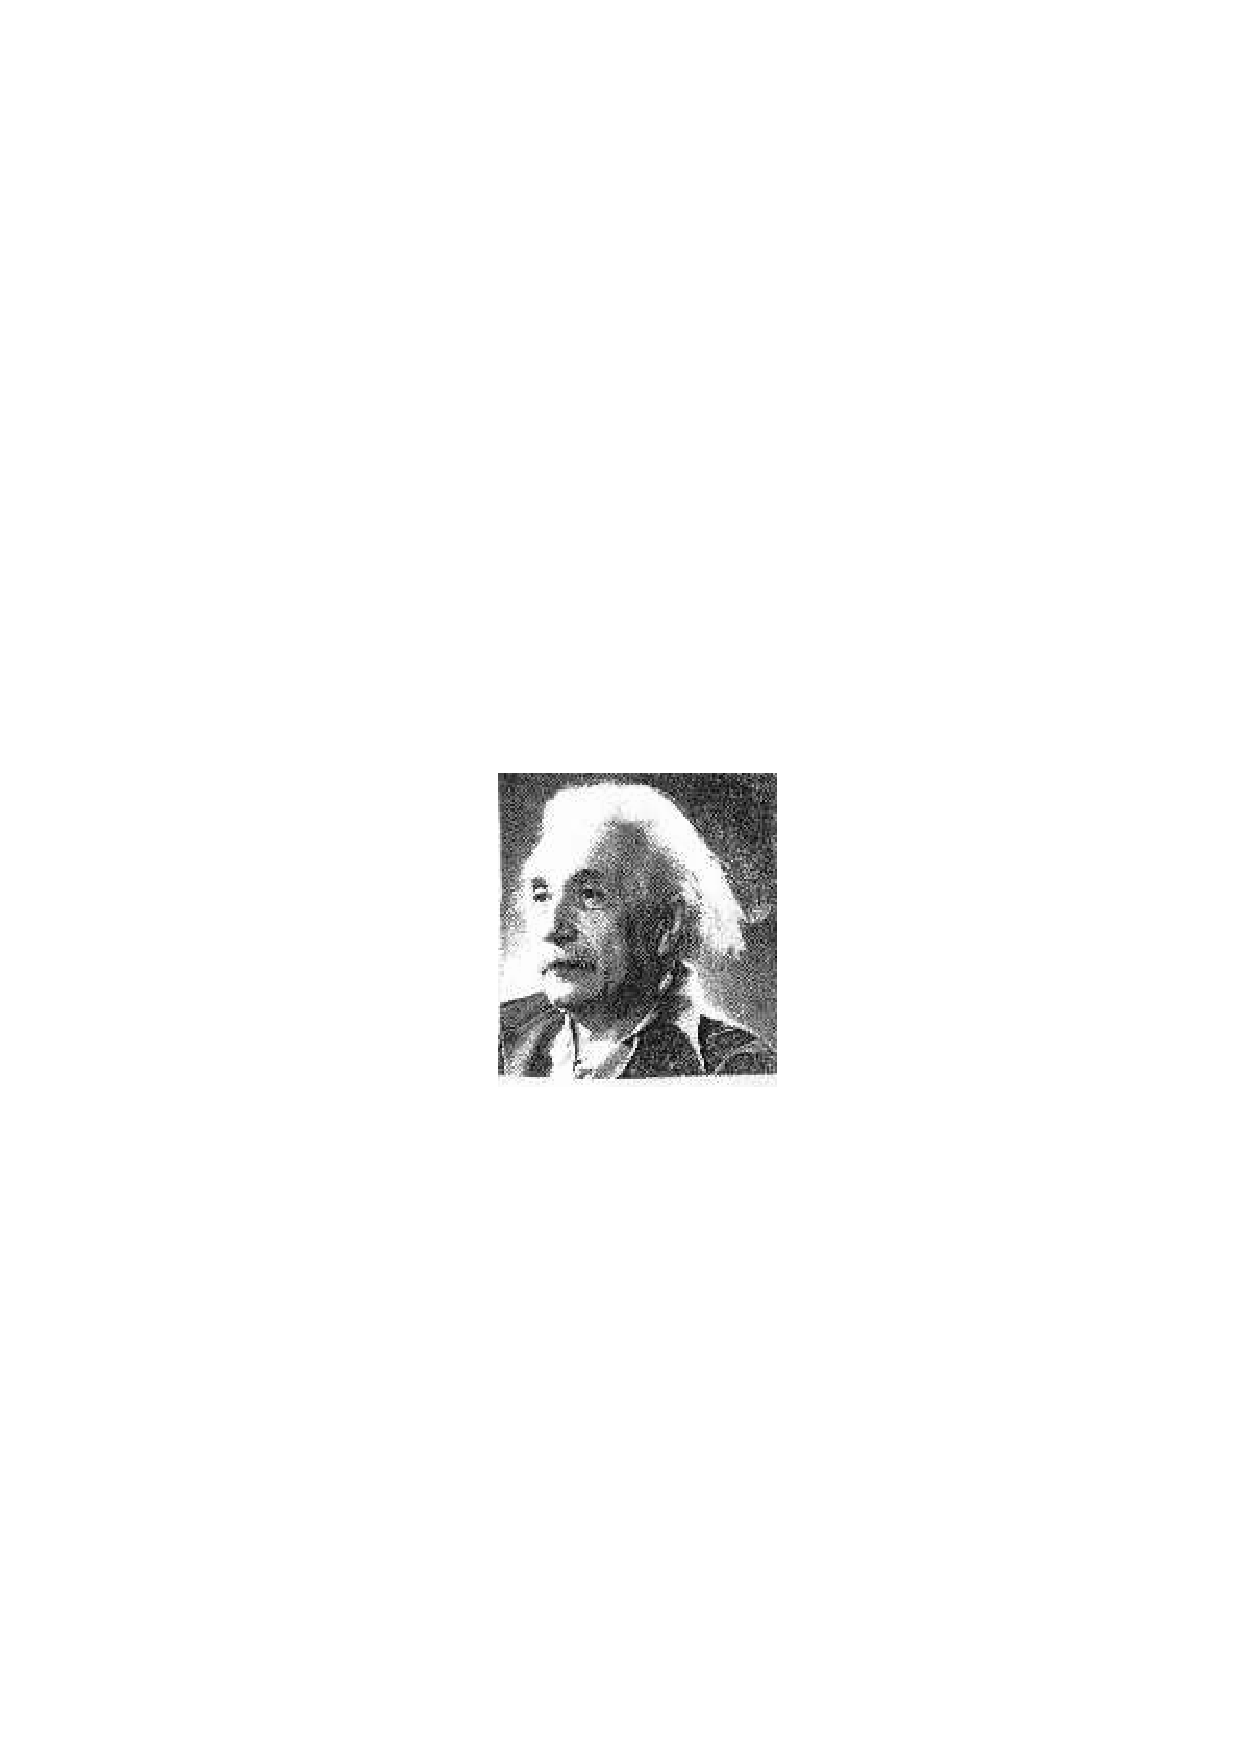
\includegraphics[width=3ex]{figsGeneric/Einstein.jpg}
\vspace{0ex}}
\hspace{0ex} 
}

\newcommand{\Einstein}{
\parbox{7mm}{\vspace{2mm}
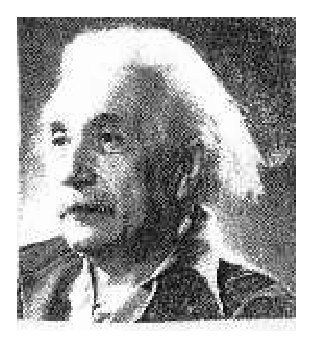
\includegraphics[width=10mm]{figsGeneric/Einstein.eps}
\vspace{-3mm}}\vspace{-3mm}
\hspace{2mm} 
}

\newcommand{\EinsteinLarge}{
\parbox{15mm}{\vspace{2mm}
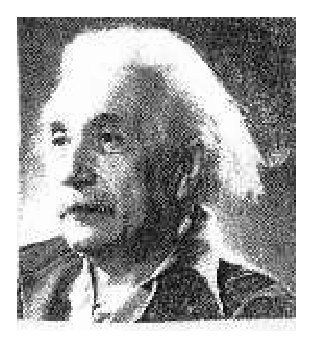
\includegraphics[width=18mm]{figsGeneric/Einstein.eps}
\vspace{-2mm}}\vspace{-2mm}
\hspace{2mm} 
}



\providecommand{\EinsteinBeg}{
\vspace{-3mm}

\Einstein
\vspace{3mm}

}

\newcommand{\OK}{\ 
\includegraphics[width=1.2em]
   {$HOME/tex/inputs/figsGeneric/OK.png}}
\newcommand{\OKeps}{
\includegraphics[width=1.2em]
   {$HOME/tex/inputs/figsGeneric/OK.eps}}
\newcommand{\contradiction}{
  \parbox{1.2em}{\vspace*{-0.2em}
  \includegraphics[width=0.9em, origin=br]
   {$HOME/tex/inputs/figsGeneric/contradiction.png}\vspace*{0.2em}}
}
\newcommand{\contradictioneps}{
  \parbox{1.2em}{\vspace*{-0.2em}
  \includegraphics[width=0.9em, origin=br]
   {$HOME/tex/inputs/figsGeneric/contradiction.eps}\vspace*{0.2em}}
}

\newcommand{\male}{\includegraphics[height=1em]
   {$HOME/tex/inputs/figsGeneric/male.eps}}
\newcommand{\female}{\includegraphics[height=1em]
   {$HOME/tex/inputs/figsGeneric/female.eps}}

\newcommand{\malepng}{\includegraphics[height=1em]
   {$HOME/tex/inputs/figsGeneric/male.png}}
\newcommand{\femalepng}{\includegraphics[height=1em]
   {$HOME/tex/inputs/figsGeneric/female.png}}

\newcommand{\circlei}{
  \parbox{1.2em}{\vspace*{-0.2em}
  \includegraphics[width=1.2em, origin=br]
   {$HOME/tex/inputs/figsGeneric/1circle.eps}\vspace*{0.2em}}
}

\newcommand{\circleii}{
  \parbox{1.2em}{\vspace*{-0.2em}
  \includegraphics[width=1.2em, origin=br]
   {$HOME/tex/inputs/figsGeneric/2circle.eps}\vspace*{0.2em}}
}

\newcommand{\circleiii}{
  \parbox{1.2em}{\vspace*{-0.2em}
  \includegraphics[width=1.2em, origin=br]
   {$HOME/tex/inputs/figsGeneric/3circle.eps}\vspace*{0.2em}}
}

\newcommand{\circleiv}{
  \parbox{1.2em}{\vspace*{-0.2em}
  \includegraphics[width=1.2em, origin=br]
   {$HOME/tex/inputs/figsGeneric/4circle.eps}\vspace*{0.2em}}
}

\newcommand{\circlev}{
  \parbox{1.2em}{\vspace*{-0.2em}
  \includegraphics[width=1.2em, origin=br]
   {$HOME/tex/inputs/figsGeneric/5circle.eps}\vspace*{0.2em}}
}


%******************************************************************
% General defs for tables
%******************************************************************

\providecommand{\titlebox}[1]{\parbox{140mm}{\vspace{2mm} #1 \vspace{2mm}}}

% top/bottom lines of the tables too close
\providecommand{\spacelinebot}[1]{\parbox[t]{1mm}{\hspace{1mm}\vspace{#1}}}
\providecommand{\spacelinetop}[1]{\parbox[b]{1mm}{\hspace{1mm}\vspace{#1}}}
\providecommand{\spacelinemid}[1]{\parbox[c]{1mm}{\hspace{1mm}\vspace{#1}}}
\providecommand{\spacingbot}{\parbox[t]{1mm}{\hspace{1mm}\vspace{3mm}}}
\providecommand{\spacingtop}{\parbox[b]{1mm}{\hspace{1mm}\vspace{6mm}}}
\providecommand{\spacingmid}{\parbox[c]{1mm}{\hspace{1mm}\vspace{9mm}}}



%******************************************************************
% General defs for figures                                        *
%******************************************************************

\providecommand{\icon}[1]{
  \parbox{7mm}{\vspace{2mm}
    \includegraphics[width=7mm]{#1}
    \vspace{-3mm}
  }
  \vspace{-3mm}
\hspace{1mm} }

% ex: \fig{0.9\textwidth}{epsfile}
\providecommand{\fig}[2]{
   \begin{center}
     \includegraphics[width=#1]{#2}
   \end{center}
}
\providecommand{\figSimple}[2]{
     \includegraphics[width=#1]{#2}
}

% ex: \figBox{0.9\textwidth}{epsfile}
% figure with parbox; necessary to make horizontal placement of figures/text
% without latex bugs
\providecommand{\figBox}[2]{
  \parbox{#1}{
     \begin{center}
     \includegraphics[width=#1]{#2}
    \end{center}
  }
}

% ex: \figBox{0.9\textwidth}{epsfile}{text}

\providecommand{\figBoxText}[3]{
  \parbox{#1}{
     \begin{center}
     \includegraphics[width=#1]{#2}
     \end{center}
     #3
  }
}

\providecommand{\oldfigc}[2]{
   \renewcommand{\baselinestretch}{1.0}
   \parbox[t]{#1}{\sloppy \small #2}
   \renewcommand{\baselinestretch}{\usualstretch}
   \small \normalsize
   }


% ex: \figps{110mm}{psfile}

\providecommand{\figps}[2]{
   \begin{minipage}[]{#1}
       \epsfxsize #1
       \epsffile{#2}
   \end{minipage}
   }

\providecommand{\figcaption}[3]{
   \renewcommand{\baselinestretch}{1.0} 
   \noindent
   \parbox[]{#1}
      {\sloppy \small Figure #2 \ 
       #3
       }
    \renewcommand{\baselinestretch}{\usualstretch}
    \small \normalsize
   }

% ex: \largefig{filename}{5mm}{\label}{captiontext}

\providecommand{\largefig}[4]{    % left fig, right text
   \begin{minipage}{\lenxtot}
       \figps{\lenxtot}{#1}
       \vspace{#2} \\
       \figcaption{\lenxtot}{#3}{#4}
   \end{minipage}
   }

% ex: \smallfig{\lenxa}{filename}{\lenxb}{\label}{captiontext}

\providecommand{\smallfig}[5]{    % left fig, right text
   \begin{minipage}{\lenxtot}
       \begin{minipage}{#1}
         \figps{#1}{#2}
       \end{minipage}
       \hfill
       \begin{minipage}{#3}
         \figcaption{#3}{#4}{#5}
       \end{minipage}
   \end{minipage}
   }


%******************************************************************
% General macros for math expressions                             *
%******************************************************************

\providecommand{\Int}{\int\limits}
\providecommand{\Sum}{\sum\limits}

\providecommand{\bfall}\textbf{\boldmath } % usual text AND math (after$)
\providecommand{\bfmath}[1]{\mbox{\textbf\boldmath{$#1$}}} % italics+fett!
\providecommand{\fett}\textbf{\boldmath } % usual text AND math (after$)

\providecommand{\dd}{{\textrm d}} %example \dd f/\dd x
\providecommand{\diff}[1]{ \ {\textrm d} #1 \, } % dx: differential operator d roman!
\providecommand{\dif}{\mathrm d} %example \dif f/\dif x
\providecommand{\e}{\mathrm e}   % example: \e^x
%!! Achtung: part, dp etc alles reservierte Befehle!!
\providecommand{\ablpart}[2]{\frac{\partial #1}{\partial #2}}  %d(#1)/d(#2)
\providecommand{\abl}[2]   {\frac{{\textrm d} #1}{{\textrm d} #2}}  % =\abltot
\providecommand{\abltot}[2]{\frac{{\textrm d} #1}{{\textrm d} #2}}  % d(#1)/d(#2)
\providecommand{\ablpartzwei}[2]{\frac{\partial^{2} #1}{\partial #2^{2}}} 
\providecommand{\ablparttwo}[2]{\frac{\partial^{2} #1}{\partial #2^{2}}} 
\providecommand{\ablpartmix}[3]{\frac{\partial^{2} #1}
           {\partial  #2 \ \partial #3}}
\providecommand{\ablpartmixed}[3]{\frac{\partial^{2} #1}
           {\partial  #2 \ \partial #3}}
\providecommand{\ablzwei}[2]{\frac{{\textrm d}^{2} #1}{{\textrm d} #2^{2}}} 

\providecommand{\cc}{^{\ast}}         %konj. komplex 
\providecommand{\complex}{C \hspace*{-0.65 em}
   \parbox{3mm}{\vspace*{-0.2 em} {\scriptsize /}}
    }
\providecommand{\cov}{\mbox{cov}}
\providecommand{\Cov}{\mbox{Cov}} %gross Cov!

\renewcommand{\d}[1]{\partial_{#1}}              %Diff.-operator
\providecommand{\deltat}{\mbox{$\delta(t-t')$}}
\providecommand{\deltar}{\mbox{$\delta(\v{r}-\v{r'})$}}
\providecommand{\deltax}{\mbox{$\delta(x-x')$}}
\providecommand{\deltavx}{\mbox{$\delta(\v{x}-\v{x}')$}}
\providecommand{\deltay}{\mbox{$\delta(y-y')$}}
\providecommand{\deltaz}{\mbox{$\delta(z-z')$}}
\providecommand{\deltart}{\mbox{$\delta(\v{r}-\v{r'})\delta(t-t')$}}
\providecommand{\deltaxyt}{\mbox{$\delta(x-x')\delta(y-y')\delta(t-t')$}}
\providecommand{\deltaij}{\mbox{$\delta_{ij}$}}
\providecommand{\deltaik}{\mbox{$\delta_{ik}$}}
\providecommand{\deltail}{\mbox{$\delta_{il}$}}
\providecommand{\deltajk}{\mbox{$\delta_{jk}$}}
\providecommand{\deltajl}{\mbox{$\delta_{jl}$}}
%arne klappt nicht:
%\providecommand{\dfrac}[2]{{\displaystyle \frac{#1}{#2}}}
\providecommand{\dsumi}{{\displaystyle \sum\limits_{i=1}^{n}}} %Summe im D-stil
\providecommand{\dint}[2]{{\displaystyle\int\limits_{#1}^{#2}}}
\providecommand{\dsum}[2]{{\displaystyle \sum\limits_{#1}^{#2}}}
\providecommand{\dsuml}[2]{{\displaystyle \sum\limits_{#1}^{#2}}} %Summe im D-stil
%\providecommand{\erw}[1]{\mbox{$\left \langle #1 \right \rangle$}} %Erwartungswert
\providecommand{\erw}[1]{\mbox{$E \left( #1 \right )$}} %Erwartungswert
\providecommand{\erf}[1]{\ \mbox{erf} \ #1} %Error function
\providecommand{\floor}[1]{{\textrm floor}\left(#1\right)}
\providecommand{\funkint}[1]{\int \!\!\cal{D}[#1]}
\providecommand{\hc}{^{\dagger}}         %konj. komplex 
\renewcommand{\Im}{\mbox{Im}}                  
\providecommand{\intd}[1]{\int \!d#1}
\providecommand{\intdn}[1]{\int \!\!d^{n}\v{#1}}
\providecommand{\intvol}{\int \!\!d^{3}} %keine Zahlen (d3) moegl.
\providecommand{\intvolr}{\int \!\!d^{3} r} %keine Zahlen (d3) moegl.
%\providecommand{\le}{\stackrel{<}{=}}   % less or equal
 
\providecommand{\nab}{\v{\nabla}}
\providecommand{\order}[1]{{\cal O}(#1)}
\providecommand{\overdot}[1]{\stackrel{.}{#1}}        
\renewcommand{\Re}{\mbox{Re}}                      
\providecommand{\re}{\mbox{Re}}                       
\providecommand{\rot}[1]{\v{\nabla}\times \v{#1}}
\providecommand{\sigeps}{\sigma_{\epsilon}}
\providecommand{\hatbeta}{\hat{\beta}}
\providecommand{\hatvec}[1]{\hat{\vec{#1}}}
\providecommand{\vecbeta}{\vec{\beta}}
\providecommand{\bfbeta}{\bfmath{\beta}}
\providecommand{\tilvecx}{\tilde{\vec{x}}}
\providecommand{\tilx}{\tilde{x}}
\providecommand{\hatvecbeta}{\hat{\vec{\beta}}}
\providecommand{\hatsigeps}{\hat{\sigma}_{\epsilon}}
\providecommand{\veceps}{\vec{\epsilon}}
\providecommand{\hatveceps}{\hat{\vec{\epsilon}}}
\providecommand{\hatsigy}{\hat{\sigma}_{y}}
\providecommand{\hatsig}{\hat{\sigma}}
\providecommand{\sumi}{\sum_{i=1}^n}
\renewcommand{\theta}{\vartheta} % zwei Arten von kleinen Thetas, ich
                                % will eins

\providecommand{\sub}[1]{dummy}
\providecommand{\sup}[1]{dummy}
% !! in some latex settings  \hspace{-0.8ex}, in some  \hspace{-0.0ex} right!
%\renewcommand{\sub}[1]{_{\text{{\scriptsize \hspace{-0.8ex}#1}}}}
%\renewcommand{\sup}[1]{^{\text{{\scriptsize \hspace{-0.8ex}#1}}}}
%\renewcommand{\sub}[1]{_{\text{{\scriptsize \hspace{-0.4ex}#1}}}}
%\renewcommand{\sup}[1]{^{\text{{\scriptsize \hspace{-0.4ex}#1}}}}
\renewcommand{\sub}[1]{_{\text{{\scriptsize \hspace{-0.0ex}#1}}}}
\renewcommand{\sup}[1]{^{\text{{\scriptsize \hspace{-0.0ex}#1}}}}
%\renewcommand{\sub}[1]{_{\rm \hspace{-0.0ex}#1}} %bug if \sub{\"OV} etc
%\renewcommand{\sup}[1]{^{\rm \hspace{-0.0ex}#1}}
%\providecommand{\tr}{^{\!\text{\scriptsize{T}}}}
\providecommand{\tr}{'}
\providecommand{\ueber}[2]{
  \left(\begin{array}{c}
     #1  \\ #2
  \end{array} \right)
}
\providecommand{\tilL}{\tilde{L}}



%\renewcommand{\vec}[1]{\mathbf{#1}}
\renewcommand{\vec}[1]{\text{\boldmath{$#1$}} }
\renewcommand{\bfmath}[1]{\text{\boldmath{$#1$}} }


%\renewcommand{\v}[1]{\mbox{\boldmath$#1$}}     %Vektor = fett
\renewcommand{\v}[1]{\vec{#1}}  %Vektorpfeil/fett je nach obigem renewcommand
%\renewcommand{\v}[1]{\bbox{#1}}     %Vektor = fett, revtex
%\renewcommand{\v}[1]{\underline{#1}} %Vektor = unterstrichen
\providecommand{\vscript}[1]{\mbox{{\scriptsize $\textbf #1$}}} % NOT for greek!


%\providecommand{\m}[1]{\underline{\v{#1}}}                  %Matrix
%\providecommand{\m}[1]{\underline{\underline{#1}}}           %Matrix
\providecommand{\m}[1]{\textbf{\textsf{#1}}\, } %Matrix=fett+gerade(nicht gr)
\providecommand{\mgr}[1]{\text{\boldmath {$#1$}}}  %Matrix griech. \sigma etc


\providecommand{\varabl}[2]{\frac{\delta #1}{\delta #2}}  %d(#1)/d(#2)

%******************************************************************
%      Independent vars etc.                                      *
%******************************************************************
 

\providecommand{\vonx} {\mbox{$(\v{x})$}}                   %(x)
\providecommand{\vonk} {\mbox{$(\v{k})$}}                   %(k)
\providecommand{\vonw} {\mbox{$(\omega )$}}                   %(omega)
\providecommand{\vonr} {\mbox{$(\v{r})$}}                   %(r)
\providecommand{\vonrs} {\mbox{$(\v{r'})$}}                   %(r')
\providecommand{\vonxyt} {\mbox{$(x,y,t)$}}                   %(x,y,z)
\providecommand{\vongrad} {\mbox{$(\v{\nabla })$}}            %(nabla)
\providecommand{\vonrgrad} {\mbox{$(\v{r},\v{\nabla })$}}     %(r,nabla)
\providecommand{\vonxt} {\mbox{$(\v{x},t)$}}                %(x,t)
\providecommand{\vonrt} {\mbox{$(\v{r},t)$}}                %(r,t)
\providecommand{\vonrsts} {\mbox{$(\v{r'},t')$}}                %(r',t')

%******************************************************************
% Misc.                                                           *
%******************************************************************
\providecommand{\nonu} {\nonumber}
\providecommand{\uu}[1]{\underline{\underline{#1}}} 
\providecommand{\COii}{\text{CO}$_2$}


%******************************************************************
% End general defs                                                *
%******************************************************************




%%% Local Variables: 
%%% mode: latex
%%% TeX-master: t
%%% End: 


%#####################################################
% Hyperlink
%#####################################################
\usepackage{units} %\unit[3]{m/s^2} => 3 m/s^2 etc!
\usepackage{eurosym}  %Euro-Symbol: \euro{Zahl} oder euro{}

%implements blocks: \begin{addmargin}[1em]{0em}% 1em left, 2em right
\usepackage{scrextend} 

\usepackage{hyperref}
% nternet-Link: \href{http://www.WasAuchImmer.html}
% {\blue{\underline{TextDesLinks} }}
% Lokaler Link: \hyperlink{targetName}{TextDesLinks}
% Link-Target: \hypertarget{targetName}

% Lokale Links: mark target with e.g. 
% \hypertarget{fig:IDM}{Target mit label fig:IDM}
% and link to it with \myLocalLink{fig:IDM}{Link zu Target fig:IDM}
\providecommand{\myHyperlink}[2]{\href{#1}{\blue{\underline{#2}}}}
\providecommand{\myLocalLink}[2]{\hyperlink{#1}{\blue{\underline{#2}}}}

%###################################################################
% bibliography-hack to put citation in my order and at several places
%###################################################################

% * need name-oriented citation style such that citation 
%   can be attributed, e.g., \bibliographystyle{elsarticle-harv}

% * compile normally with bibtex and enter resulting .bbl file
%   manually at appropriate places (commenting out bib commands)

% * remove \bibliography{...} and compile ONCE (at the second time, we
% get ?? in the citation places)

\newcommand{\mybibentry}[1]{
\parindent0em
\hspace{2em}
\parbox{0.95\textwidth}{
\parindent-2em
#1
\vspace{1ex}
}

}


% use no-link generation for cite and citep because they are broken
% as a side effect

\newcommand*{\nolinkcite}[1]{%
  {\protect\NoHyper\cite{#1}\protect\endNoHyper}%
}
\newcommand*{\nolinkcitep}[1]{%
  {\protect\NoHyper\citep{#1}\protect\endNoHyper}%
}

% end bibliography-hack to put citation in my citation order 
% and at several places
%########################################################


%#####################################################
% Preprint vs. Publikation
%#####################################################
\providecommand{\martin}[1]{\green{Martin: #1}} %Preprint
%\providecommand{\martin}[1]{}                  %fuer Veroeffentlichung
\providecommand{\arne}[1]{\green{Martin: #1}}   %Preprint
%\providecommand{\arne}[1]{}                    %fuer Veroeffentlichung


%#####################################################
% latest changes from Arne
%#####################################################

% 8-10-04: ex: \includefig{110mm}{psfile}
\newcommand{\includefig}[2]{\includegraphics[width=#1]{#2}}
\providecommand{\bra}{\langle}
\providecommand{\ket}{\rangle}
%#####################################################
% defs of Arne
%#####################################################

\providecommand{\uul}{\uu}
\providecommand{\ug}{\approx}  % ungefaehr gleich
\providecommand{\nor}[1]{\mathrm{#1}}
\providecommand{\sollsein}{\,{\stackrel{!}{=}}\,}
\providecommand{\binom}[2]{\ueber{#1}{#2}}
\providecommand{\www}[1]{\texttt{#1}}
\providecommand{\mytilde}{\symbol{126}} % ist die Tilde!!!
\providecommand{\etal}{\textit{et al.}}
%
\providecommand{\cl}[1]{{\centering #1}}
\providecommand{\no}{\noindent}  % keine Einr�ckung bei neuer Zeile
%
\providecommand{\bno}{\begin{equation*}}   % no citation number
\providecommand{\eno}{\end{equation*}}

\providecommand{\also}{$\to\,$}
\providecommand{\kasten}[1]{\begin{displaymath}\fbox{$\quad\displaystyle #1\quad$}\end{displaymath}}
\providecommand{\ul}[1]{\underline{#1}}   
\providecommand{\uu}[1]{\underline{\underline{#1}}}  % bereits in latex def!
\providecommand{\uul}{\uu}
\providecommand{\ol}[1]{\overline{#1}} 
%fuer mich:
%irgendwie mit german schon definiert !?
\providecommand{\3}{{\ss }}



%******************************************************************
%  General definitions for latex, revtex
%******************************************************************
\renewcommand{\ae}{{\"a}\hspace{-0.4em}}
\renewcommand{\oe}{{\"o}\hspace{-0.4em}}
\providecommand{\ue}{{\"u}\hspace{-0.4em}}
\providecommand{\Ae}{{\"A}\hspace{-0.4em}}
\providecommand{\Oe}{{\"O}\hspace{-0.4em}}
\providecommand{\Ue}{{\"U}\hspace{-0.4em}}


% to circumvent a bug that euro symbols are not displayed in math mode
\providecommand{\eur}{\text{\euro{}}}


\providecommand{\IR}{I\!\!R}
\providecommand{\IN}{I\!\!N}

\providecommand{\lowtilde}{{\mbox{$_{\tilde{}}$}}}
\providecommand{\backsl}{\mbox{$\backslash\!$}}




%##################################################
% colors
%##################################################

% defines {\black ...}, {\red ...}, ... and
%\black{} \red{} \green{} \turk{} \viol{} \orange{}
% \brown{} \grey{}
% visible only in ps not in dvi! (=>tex2ps <texfile w/o ext>)

%\usepackage[dvips]{color} %!! sometimes ``option clash''=> def w/o options
\usepackage{color}

\definecolor{black}{rgb}{0,0,0}
\definecolor{red}{rgb}{0.8,0,0}
\definecolor{lightred}{rgb}{1,0.5,0.5}
\definecolor{green}{rgb}{0,0.8,0}
\definecolor{blue}{rgb}{0,0,1}
\definecolor{turk}{rgb}{0,1,1}
\definecolor{viol}{rgb}{1,0,1}
\definecolor{orange}{rgb}{1,0.4,0.}
\definecolor{yellow}{rgb}{1,0.7,0.}
\definecolor{brown}{rgb}{0.7,0.4,0}
\definecolor{gray}{rgb}{0.7,0.7,0.7}
\definecolor{darkgray}{rgb}{0.5,0.5,0.5}
\definecolor{lightgray}{rgb}{0.95,0.95,1.0}
\definecolor{verylightred}{rgb}{1,0.7,0.5}

\definecolor{TUDblue1}{rgb}{.05,.22,.410}
\definecolor{TUDblue2}{rgb}{.11, .42, .81}
\definecolor{mygreen}{rgb}{0.,0.4,0.4}
\definecolor{myred}{rgb}{1,0.0,0.0}
\definecolor{blueTUD}{rgb}{0.1,0,0.5} %my color

%% !! only so cumbersome. Short search: 
% No shortcut defining rgb directly (nov19)

\providecommand{\verylightred}[1]{\textcolor{verylightred}{#1}}
\providecommand{\black}[1]{\textcolor{black}{#1}}
\providecommand{\red}[1]{\textcolor{red}{#1}}
\providecommand{\blue}[1]{\textcolor{blue}{#1}}
\providecommand{\green}[1]{\textcolor{green}{#1}}
\providecommand{\turk}[1]{\textcolor{turk}{#1}}
\providecommand{\viol}[1]{\textcolor{viol}{#1}}
\providecommand{\orange}[1]{\textcolor{orange}{#1}}
\providecommand{\yellow}[1]{\textcolor{yellow}{#1}}
\providecommand{\brown}[1]{\textcolor{brown}{#1}}
\providecommand{\gray}[1]{\textcolor{gray}{#1}}
\providecommand{\lightgray}[1]{\textcolor{lightgray}{#1}}
\providecommand{\lightred}[1]{\textcolor{lightred}{#1}}

\newcommand{\myred}[1]{{\color{myred} #1}}
\newcommand{\myblue}[1]{{\color{TUDblue1} #1}}
\newcommand{\mygreen}[1]{{\color{mygreen} #1}}
\newcommand{\blueTUD}[1]{{\color{blueTUD} #1}}  %my color
\providecommand{\bfdefTUD}[1]{\hspace*{0.01em}{\boldmath \textbf{\blueTUD{#1}}}}
\providecommand{\bfblack}[1]{\hspace*{0.01em}{\boldmath \textbf{\black{ #1}}}}
\providecommand{\bfgreen}[1]{\hspace*{0.01em}{\boldmath \textbf{\green{#1}}}}
\providecommand{\bfred}  [1]{\hspace*{0.01em}{\boldmath \textbf{\red{#1}}}}
\providecommand{\bforange}[1]{\hspace*{0.01em}{\boldmath
    \textbf{\orange{#1}}}}
\providecommand{\bfyellow}[1]{\hspace*{0.01em}{\boldmath 
    \textbf{\yellow{#1}}}} 



%#################################################################
% special colors definitions for special structures in scripts/transparencies
%#################################################################

% main text
\definecolor{colMainText}{rgb}{1,0.75,0.3}
\newcommand{\colMainText}[1]{{\color{colMainText} #1}}

% main equations
\definecolor{colMainEq}{rgb}{1,0.75,0.3}
\newcommand{\colMainEq}[1]{{\color{colMainEq} #1}}


% definitions
\definecolor{colDef}{rgb}{0.6,0,0.2}
\newcommand{\colDef}[1]{{\color{colDef} #1}}
\providecommand{\bfdef}[1]{\hspace*{0.01em}{\boldmath \textbf{\colDef{#1}}}}

% questions and answers

\definecolor{colAsk}{rgb}{1,0.5,0.}
\newcommand{\colAsk}[1]{{\color{colAsk} #1}}

\definecolor{colAnswer}{rgb}{0,0.5,0.5}
\newcommand{\colAnswer}[1]{{\color{colAnswer} #1}}

\providecommand{\bfAsk}[1]{\hspace*{0.01em}{\boldmath \textbf{\colAsk{#1}}}}
\providecommand{\bfAnswer}[1]{\hspace*{0.01em}{\boldmath
    \textbf{\colAnswer{#1}}}}

\providecommand{\itemAsk}{\item[\bfAsk{?}]}
\providecommand{\itemAnswer}{\item[\bfAnswer{!}]}

% comments before '=' signs in calculation steps
% example: 
% \bdma S &=& (AB)C \\ \remark{associativity} &=& ABC \edma
\providecommand{\remark}[1]{\text{\scriptsize{\red{[#1 $\to$]}}}}

%#################################################################

\newcommand{\rlogo}[1]{\hfill {\color{black} {\texttt{#1.}}} \hspace*{-3mm} \includegraphics[width=4mm]{../style/Rlogo}}

%###########################################################
% absolute positioning of boxes or images
%###########################################################


% https://tex.stackexchange.com/questions/311007/change-package-option-overlay-from-textpos-package-in-document/311031#311031

\usepackage{tikz}
\usetikzlibrary{calc}
\newcommand{\placebox}[4][center]{%
  % [#1]: box anchor: center (default) | 
  %                 south west | west | north west | north |
  %                 north east | east | south east | south | 
  %                 mid west | mid | mid east |
  %                 base west | base | base east 
  % #2: horizontal position (fraction of page width)
  % #3: vertical position (fraction of page height)
  % #4: content
  %
  \tikz[remember picture,overlay,x=\paperwidth,y=\paperheight]{%
    \node[anchor=#1,inner sep=0pt]
    at ($(current page.south west)+(#2,#3)$) {#4};
  }%
}
%###########################################################

% make images pale (see demo_makePale.tex)
%\makePale{opacity}{centerXrel}{centerYrel}{wrel}{hrel}
% e.g., \makePale{0.6}{0.5}{0.5}{1}{0.3}

\usepackage{pgfcore}

\providecommand{\makePale}[5]{
 \setlength{\unitlength}{0.5\textwidth}
 \placebox{#2}{#3}{
   \begin{picture}(0,0)
   \put(-#4,-#5){
    \pgfsetfillopacity{#1}{
     \textcolor{white}{\rule{#4\textwidth}{#5\textheight}}
    }
   }
   \end{picture}
 }
}

%###########################################################



%usage \circled{2} gives 2 in a circle

\newcommand*\circled[1]{\tikz[baseline=(char.base)]{
    \node[shape=circle, draw, inner sep=1pt, 
        minimum height=12pt] (char) {#1};}}





% example own definition
\definecolor{lyellow}{rgb}{1,1,0.5}
\providecommand{\lyellow}[1]{\textcolor{lyellow}{#1}}
\definecolor{lblue}{rgb}{0.91,1,1}
\providecommand{\lblue}[1]{\textcolor{lblue}{#1}}

% (jul19, old notebook) ACHTUNG: \textsf{ statt \sffamily{ DOS !!

% find keywords: caption, title
\providecommand{\bfsf}[1]{\large{\sffamily\textbf{#1}}}
\providecommand{\secfont}[1]{\Large{\sffamily\textbf{#1}}}
\providecommand{\myheading}[1]{\Large{\sffamily\textbf{\blueTUD{#1}}}}
\providecommand{\mysubheading}[1]{\large{\sffamily\textbf{\blueTUD{#1}}}}
\providecommand{\mysubsubheading}[1]{\sffamily\textbf{\blueTUD{#1}}}


%******************************************************************
% General defs for structural units and environments 
%******************************************************************

% see also \mysubheading etc

\providecommand{\mysection}[1]   {\section{{\textsf\Large\textbf{#1}}}}
\providecommand{\mysubsection}[1]{\subsection{{\textsf\large\textbf{#1}}}}

% fuer usepackage[a4paper]{foils}  (sonst Headings groe\3er)
%calling sequence: \myfigure{title}{images}{explanatory text}
\providecommand{\myfigure}[3]{
%\newpage
\begin{center}
{\large\textsf\textbf{#1}} \\[-4mm]
\end{center}
#2

#3
}


\providecommand{\bc}{\begin{center}}
\providecommand{\ec}{\end{center}}
\providecommand{\be}{\begin{equation}}
\providecommand{\ee}{\end{equation}}
\providecommand{\bea}{\begin{eqnarray}}
\providecommand{\eea}{\end{eqnarray}}
\providecommand{\bdm}{\begin{displaymath}}
\providecommand{\edm}{\end{displaymath}}
\providecommand{\bdma}{\begin{eqnarray*}}
\providecommand{\edma}{\end{eqnarray*}}
\providecommand{\ba}{\begin{eqnarray*}}
\providecommand{\ea}{\end{eqnarray*}}
\providecommand{\bi}{\begin{itemize}}
\providecommand{\ei}{\end{itemize}}
\providecommand{\benum}{\begin{enumerate}}
\providecommand{\eenum}{\end{enumerate}}


\providecommand{\dis}[1]{ {\displaystyle #1}}

%example:\dmTwo{qlhs1 &=rhs1 \\ lhs2 &=rhs2}
\providecommand{\dmTwo}[1]{
  \begin{displaymath}
    \begin{array}{ll} #1
    \end{array}
  \end{displaymath}
}
% wie bdma ... edma, aber alles linkszentriert

\providecommand{\dmThree}[1]{
  \begin{displaymath}
    \begin{array}{lll} #1
    \end{array}
  \end{displaymath}
}

%example: $ f(x)=\twoCases{0}{x<0}{1}{x\ge 0}$
\providecommand{\twoCases}[4]{
  \left\{ 
    \begin{array}{ll} 
      #1 & #2 \\
      #3 & #4 
    \end{array} 
  \right.
}
\providecommand{\threeCases}[6]{
  \left\{ 
    \begin{array}{ll} 
      #1 & #2 \\
      #3 & #4 \\ 
      #5 & #6 
    \end{array} 
  \right.
}
\providecommand{\fourCases}[8]{
  \left\{ 
    \begin{array}{ll} 
      #1 & #2 \\
      #3 & #4 \\ 
      #5 & #6 \\ 
      #7 & #8 
    \end{array} 
  \right.
}

% column vector with parentheses, e.g.,
%\myVector{1\\2\\3}

\providecommand{\myVector}[1]{
  \left(\begin{array}{c} 
      #1 
   \end{array} \right)
}

%matrix with two columns, e.g.,
% \myMatrixTwo{c11&c12\\c21&c22\\c31&c32}
%BESSER: \begin{pmatrix} c11&c12\\c21&c22\end{pmatrix}

\providecommand{\myMatrixTwo}[1]{
  \left(\begin{array}{cc} 
      #1 
   \end{array} \right)
}

%matrix with three columns, e.g.,
% \myMatrixThree{c11&c12&c13\\c21&c22&c23\\c31&c32&c33}
%BESSER: \begin{pmatrix} c11&c12\\c21&c22\end{pmatrix}

\providecommand{\myMatrixThree}[1]{
  \left(\begin{array}{ccc} 
      #1 
   \end{array} \right)
}

\providecommand{\myMatrixFour}[1]{
  \left(\begin{array}{cccc} 
      #1 
   \end{array} \right)
}

\providecommand{\myMatrixFive}[1]{
  \left(\begin{array}{ccccc} 
      #1 
   \end{array} \right)
}

\providecommand{\non}{\nonumber \\}
\providecommand{\no}{\nonumber}

\providecommand{\refkl}[1]{(\ref{#1})}

%######################################
% boxed displayed equations
%######################################

\providecommand{\fboxdm}[1]{
 \begin{center} \fbox{
   ${\displaystyle \begin{array}{l} #1 \end{array}}$} \end{center}
}

\providecommand{\fboxeq}[1]{
\begin{equation}
 \fbox{${\displaystyle  #1 }$}
\end{equation}
}


\providecommand{\fboxtext}[1]{
  \begin{center} \framebox{
    \begin{minipage}{0.8\textwidth} #1 \end{minipage}
  }
  \end{center}
}

\providecommand{\fitfboxtext}[1]{
  \begin{center} 
    \fbox{{#1}}
  \end{center}
}



%#####################################################
% Numberered equation with background color (including the numbering)
% needs colors.sty; ex.: \bgcoloreq{green}{x^2 = y^2+z^2}
\providecommand{\bgcoloreq}[2]{
  \mbox{\colorbox{#1}{
    \begin{minipage}{\textwidth}
      \begin{equation} #2 \end{equation}
    \end{minipage}
  }}
}

%###################################################
% Numberered equation with background color only behind the formula
% needs colors.sty; ex.: \bgeq{green}{label}{x^2 = y^2+z^2}

\providecommand{\bgeq}[3]{
  \begin{equation}
  \label{#2}
  \colorbox{#1}{$ {\displaystyle #3}$}
  \end{equation}
}

%###################################################
% Displayed equation with background color (over whole width)
% needs colors.sty; ex.: \bgcolordm{red}{x^2=1}
\providecommand{\bgcolordm}[2]{
  \mbox{\colorbox{#1}{
    \begin{minipage}{\textwidth}
       \vspace*{-2ex} % folg. Leerzeile wichtig; vspace nicht woanders...

       \begin{displaymath} #2 \end{displaymath}
       \vspace*{-3.8ex} % folg. Leerzeile wichtig, ... da ignoriert


    \end{minipage}
  }}
}

%###############################################
% Centered equation with background color only behind the formula
% needs colors.sty; ex.: \bgcolormath{red}{x^2=1}
\providecommand{\bgcolormathcenter}[2]{
 \begin{center}
  \colorbox{#1}{${\displaystyle #2}$}
 \end{center}
}

%###############################################
% non-centered displayed equation with background color only behind the formula
% needs colors.sty; ex.: \bgcolormath{red}{x^2=1}
\providecommand{\bgcolormath}[2]{
  \colorbox{#1}{${\displaystyle #2}$}
}


%################################################################
% Standard colored box with some margins and width=whole textwidth
% needs colors.sty; ex.: \widecolorbox{lilablassblau}{bel. Inhalt}
\providecommand{\widecolorbox}[2]{
  \mbox{\colorbox{#1}{
    \hspace*{0.5em}\begin{minipage}{0.94\textwidth}
      \vspace*{1ex}

       #2
       \vspace*{1ex}


    \end{minipage}\hspace*{0.5em}
  }}
}

\providecommand{\widecolorboxExmpl}[2]{
  \mbox{\colorbox{#1}{
    \hspace*{0.5em}\begin{minipage}{0.88\textwidth}
      \vspace*{1ex}

       #2
       \vspace*{1ex}


    \end{minipage}\hspace*{0.5em}
  }}
}

%################################################################
% Standard colored box without margins and width=whole textwidth
% needs colors.sty; ex.: \colbox{lilablassblau}{bel. Inhalt}
% NOTE: much more flexible than usual \colorbox!
\providecommand{\colbox}[2]{
  \mbox{\colorbox{#1}{
    \hspace*{0.1em}\begin{minipage}{\textwidth}
      \vspace*{0ex}

       #2
       \vspace*{0ex}


    \end{minipage}\hspace*{-0.1em}
  }}
}


%######################################
% Non-buggy multiline table entry: a component of entryExample below
% Calling sequence: \myBox{width}{text}
%######################################

\newcommand{\myBox}[2]{
  \hspace{-0.2mm}\parbox{#1}{
      \vspace*{2mm}#2\vspace*{2mm}      
  } \hspace*{-1mm}
}
 
%######################################
% Example: 3-column table with
% non-buggy multiline behaviour of the entries (as in usual latex)
% \begin{tabular}{|l|l|l|}  \hline
% \entryExample{left}{center}{right} \entry{ ....} ...
% \end{tabular}  
%######################################

\providecommand{\entryExample}[3]{
       \hspace{2mm}\parbox{40mm}{\vspace*{2mm}#1\vspace*{2mm}} \hspace*{-2mm}
     & \hspace{2mm}\parbox{30mm}{\vspace*{2mm}#2\vspace*{2mm}} \hspace*{-2mm}
     & \hspace{2mm}\parbox{30mm}{\vspace*{2mm}#3\vspace*{2mm}} \hspace*{-2mm}
                        \\ \hline
                       }


%######################################
% Example table with decimal-point centered entries:

% \usepackage{dcolumn}  % Ausrichtung an Dezimalpunkt
% \begin{tabular}{|D{.}{.}{1}|D{.}{.}{1}|D{.}{.}{1}|} \hline
% \entryDec{left}{center}{right}
% \end{tabular}  
%!! aber auch Bug: vergroessert gewaltsam Tabellen, ohne dass
% andere Nichtzahlenzeilen (Titel) dies ausnutzen koennten!
% => muss diesen Bug mit erhoehten \hspace-Werten in \entry (fuer Titel)
% ausmerzen! (anderes geht nicht!! DOS!
%######################################

\providecommand{\entryDec}[3]{
 &&\\[-4mm]                      % schafft oben mehr Platz
 #1 & #2 & #3 \\[1mm] \hline     % schafft unten mehr Platz 
}                              % ! \vspace{..} unterbr Tab, \\[] nicht!



%!! citebox:Latex-Bug: Setzt nicht kleineren Textabstand bei kleinerer Schrift
% breche laengere Eintraege gewaltsam mit \\[-4mm] um
% Bug 2: vertikaler Abstand des Zitierenden #2 oft falsch; korrigiere mit
% \vspace beim #!-Eintrag!

\providecommand{\citebox}[2]{
  \hspace*{\fill}
  \begin{minipage}{90mm}
  %\renewcommand{\baselinestretch}{1.0}
  \footnotesize {\textsl #1}
  \end{minipage}
  \vspace*{-2mm}

  \hspace*{\fill}{ \scriptsize #2 }
}

\providecommand{\citeboxi}[2]{
  \hspace*{\fill}
  \begin{minipage}{100mm}
  \renewcommand{\baselinestretch}{1.0}
  \footnotesize {\sl #1}
  \vspace*{-3mm}\\
  \hspace*{\fill} #2\\
  \end{minipage}
  }

\providecommand{\footnotespace}[1]{\footnote{\hspace{0.3em}#1}}
\providecommand{\tabsetting}{
              \renewcommand{\baselinestretch}{1.0}\small \normalsize}
\providecommand{\tabspacesetting}[1]{
              \renewcommand{\baselinestretch}{#1}\small \normalsize}


%#########################################################
% Create custom environemnts : Those used for Vkmod.tex 
%#########################################################

% usage: \begin{itemize} ... \itemgray{text} ... \end{itemize}
% beware: \colorbox{lightgray}{  .. } extends only over 1 line!
% triangle: tip up
% triangleright: tip right but not filled
% blacktriangleright: tip right, filled=OK override black by color

\providecommand{\itemgray}[1]{
{\color{darkgray}
  \item[\color{darkgray}\scalebox{0.7}{$\blacktriangleright$}] #1}
}

% usage: \aufgabenbox{caption}{text}
\providecommand{\aufgabenbox}[2]{
  \vspace{3mm}
  {\parindent0mm
  \widecolorbox{lightgray}{
    {\textsf\textbf{#1}} \vspace{3mm}

 #2
  }}
 \vspace{5mm}

}

% usage: \verstaendnisbox{text}

\providecommand{\verstaendnisbox}[1]{
  \vspace{3mm}
  {\parindent0mm
  \widecolorbox{lightgray}{
    \textbf{Verst\"andnisfrage:}\\[-8mm]
    \begin{itemize}
      \item[] #1
    \end{itemize}
  \vspace*{-2mm}
  }}
 \vspace{5mm}

}

\providecommand{\examplebox}[2]{
 \begin{center}
  \vspace{3mm}
  {\parindent0mm
  \widecolorboxExmpl{lblue}{
%  \widecolorboxExmpl{lightgray}{
    \textit{#1}\\[0.5em]
    #2
    \vspace*{0.5em}
    }
  }
  \vspace{1em}
  \end{center}
}


%\providecommand{\verstaendnisbox}[1]{
%  \vspace{5mm}
%  \textbf{Verst\"andnisfrage:}\\[-8mm]
%  \begin{itemize}
%    \item[] #1
%  \end{itemize}
%}

%usage: \maineq{eq_label}{formula}

\providecommand{\maineq}[2]{
 \bgeq{colMainEq}{#1}{#2}
}

%usage: \maindm{formula}

\providecommand{\maindm}[1]{
 \bgcolormathcenter{colMainEq}{#1}
}


\providecommand{\maindmIntext}[1]{
 \bgcolormath{colMainEq}{#1}
}

%usage: \maintextbox{width}{text}

\providecommand{\maintextbox}[2]{
\vspace{0.5mm}
\begin{center}
  \colorbox{colMainText}{
   \hspace*{0.5mm}
     \parbox{#1}{\vspace*{0.5mm}
     #2\vspace*{0.5mm}
     }
   \hspace*{0.5mm} 
  }
\end{center}
\vspace{0mm}
}

%usage: \maintext{text}

\providecommand{\maintext}[1]{
 \maintextbox{0.95\textwidth}{#1}
}

\providecommand{\maintextSimple}[1]{ % bug: no center allowed in placebox
  \colorbox{colMainText}{
   \hspace*{0.5mm}
     \parbox{0.95\textwidth}{\vspace*{0.5mm}
     #1\vspace*{0.5mm}
     }
   \hspace*{0.5mm} 
  }
}



%******************************************************************
% General defs for words, text symbols and icons
%******************************************************************
\providecommand{\text}[1]{{\mbox{ #1}}}

\providecommand{\Angstroem}{{\AA}}
\providecommand{\cels}{\mbox{$^{\circ}{\textrm C}$}}
\providecommand{\emptySet}{\{\not\hspace{-1mm}0\}}
\providecommand{\Fr}{\mbox{Fr\'{e}edericksz--}}
\providecommand{\Poincare}{Poincar\'{e}}
\providecommand{\rb}{Rayleigh--B\'{e}nard}
\providecommand{\RB}{Rayleigh--B\'{e}nard}
\providecommand{\via}{\textit{via}}
\providecommand{\msii}{\mbox{m/s$^2$}}
\providecommand{\result}[1]{\underline{\underline{#1}}}
 
\newcommand{\EinsteinPdflatex}{
\parbox{3ex}{\vspace{-0ex}
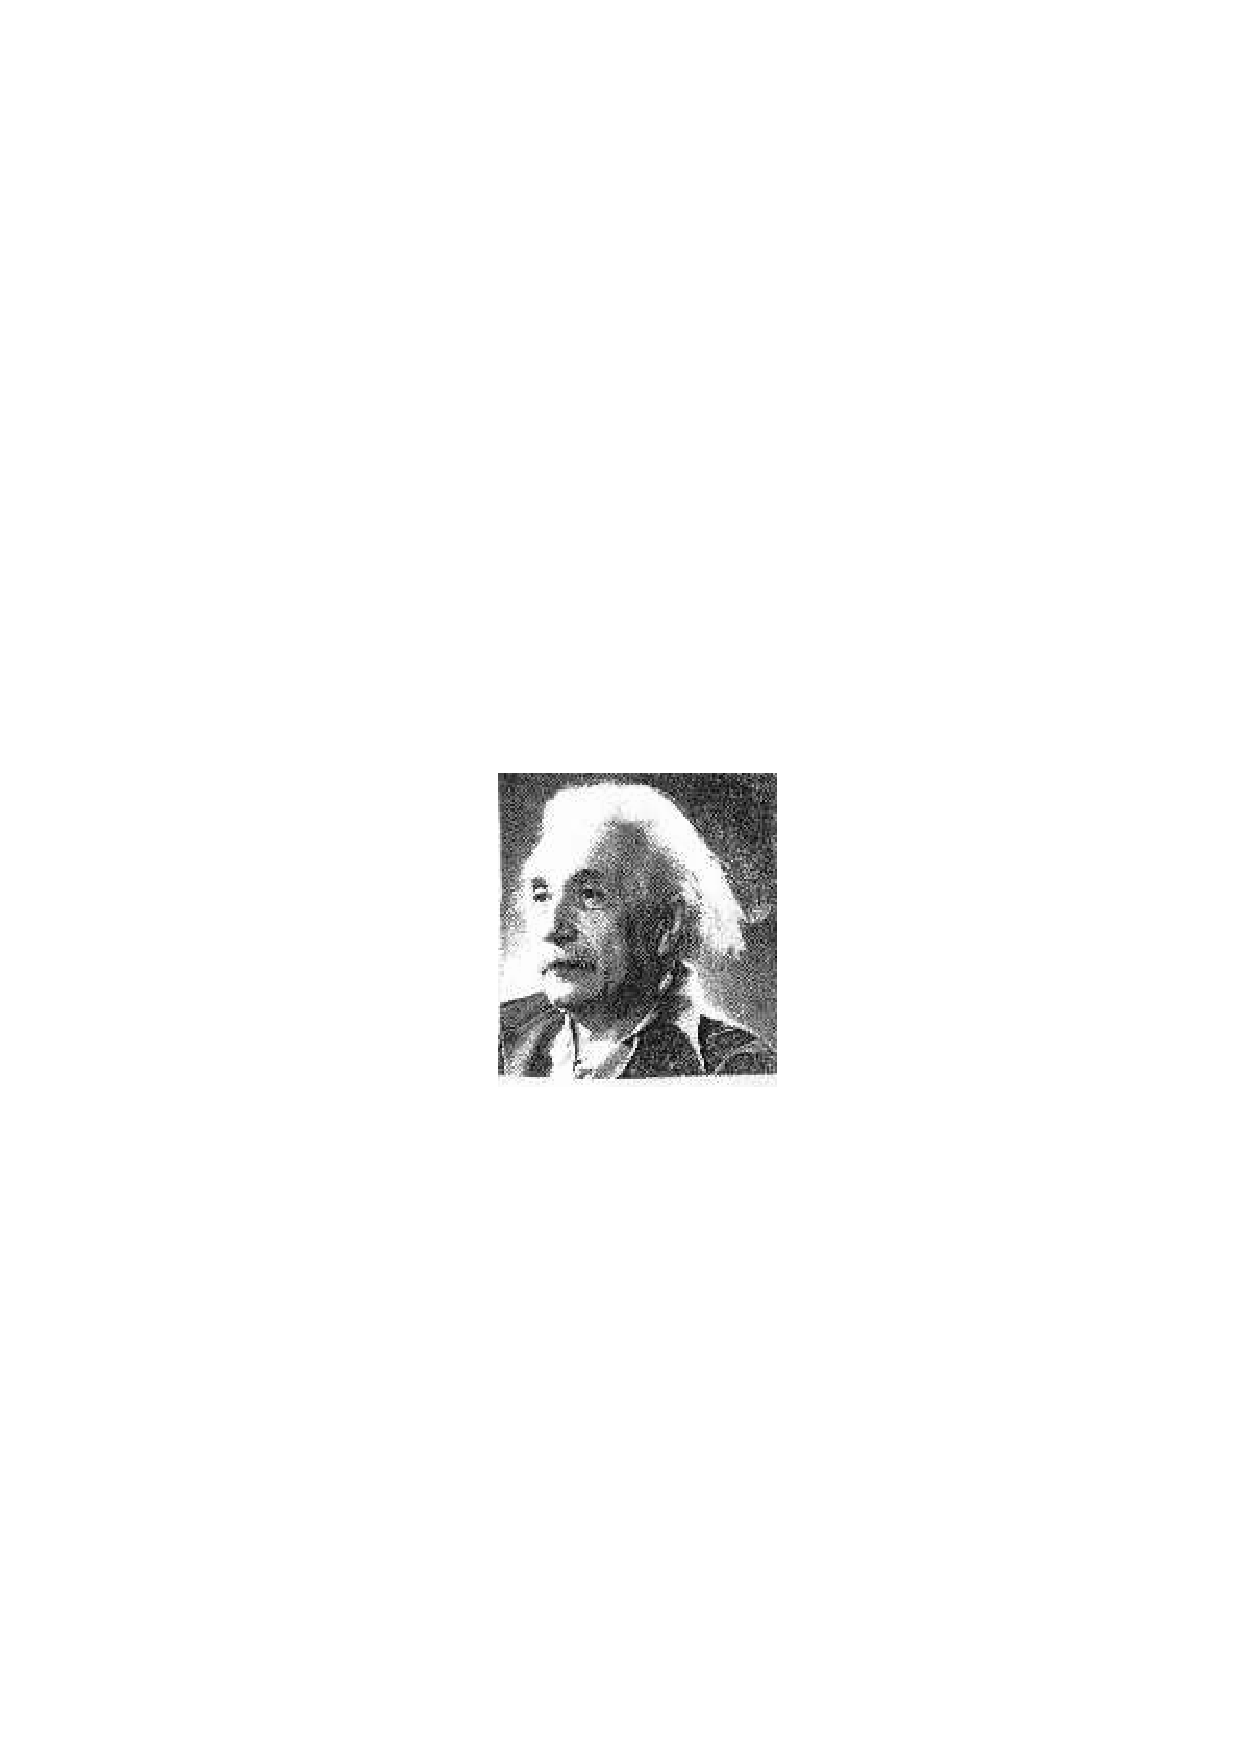
\includegraphics[width=3ex]{figsGeneric/Einstein.jpg}
\vspace{0ex}}
\hspace{0ex} 
}

\newcommand{\Einstein}{
\parbox{7mm}{\vspace{2mm}
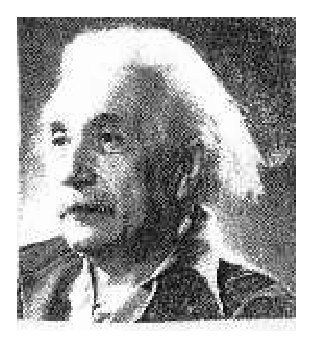
\includegraphics[width=10mm]{figsGeneric/Einstein.eps}
\vspace{-3mm}}\vspace{-3mm}
\hspace{2mm} 
}

\newcommand{\EinsteinLarge}{
\parbox{15mm}{\vspace{2mm}
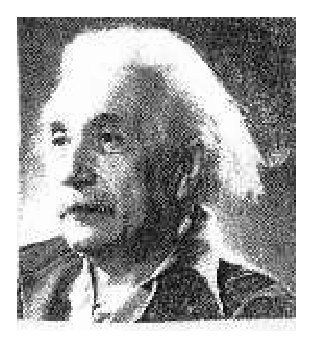
\includegraphics[width=18mm]{figsGeneric/Einstein.eps}
\vspace{-2mm}}\vspace{-2mm}
\hspace{2mm} 
}



\providecommand{\EinsteinBeg}{
\vspace{-3mm}

\Einstein
\vspace{3mm}

}

\newcommand{\OK}{\ 
\includegraphics[width=1.2em]
   {$HOME/tex/inputs/figsGeneric/OK.png}}
\newcommand{\OKeps}{
\includegraphics[width=1.2em]
   {$HOME/tex/inputs/figsGeneric/OK.eps}}
\newcommand{\contradiction}{
  \parbox{1.2em}{\vspace*{-0.2em}
  \includegraphics[width=0.9em, origin=br]
   {$HOME/tex/inputs/figsGeneric/contradiction.png}\vspace*{0.2em}}
}
\newcommand{\contradictioneps}{
  \parbox{1.2em}{\vspace*{-0.2em}
  \includegraphics[width=0.9em, origin=br]
   {$HOME/tex/inputs/figsGeneric/contradiction.eps}\vspace*{0.2em}}
}

\newcommand{\male}{\includegraphics[height=1em]
   {$HOME/tex/inputs/figsGeneric/male.eps}}
\newcommand{\female}{\includegraphics[height=1em]
   {$HOME/tex/inputs/figsGeneric/female.eps}}

\newcommand{\malepng}{\includegraphics[height=1em]
   {$HOME/tex/inputs/figsGeneric/male.png}}
\newcommand{\femalepng}{\includegraphics[height=1em]
   {$HOME/tex/inputs/figsGeneric/female.png}}

\newcommand{\circlei}{
  \parbox{1.2em}{\vspace*{-0.2em}
  \includegraphics[width=1.2em, origin=br]
   {$HOME/tex/inputs/figsGeneric/1circle.eps}\vspace*{0.2em}}
}

\newcommand{\circleii}{
  \parbox{1.2em}{\vspace*{-0.2em}
  \includegraphics[width=1.2em, origin=br]
   {$HOME/tex/inputs/figsGeneric/2circle.eps}\vspace*{0.2em}}
}

\newcommand{\circleiii}{
  \parbox{1.2em}{\vspace*{-0.2em}
  \includegraphics[width=1.2em, origin=br]
   {$HOME/tex/inputs/figsGeneric/3circle.eps}\vspace*{0.2em}}
}

\newcommand{\circleiv}{
  \parbox{1.2em}{\vspace*{-0.2em}
  \includegraphics[width=1.2em, origin=br]
   {$HOME/tex/inputs/figsGeneric/4circle.eps}\vspace*{0.2em}}
}

\newcommand{\circlev}{
  \parbox{1.2em}{\vspace*{-0.2em}
  \includegraphics[width=1.2em, origin=br]
   {$HOME/tex/inputs/figsGeneric/5circle.eps}\vspace*{0.2em}}
}


%******************************************************************
% General defs for tables
%******************************************************************

\providecommand{\titlebox}[1]{\parbox{140mm}{\vspace{2mm} #1 \vspace{2mm}}}

% top/bottom lines of the tables too close
\providecommand{\spacelinebot}[1]{\parbox[t]{1mm}{\hspace{1mm}\vspace{#1}}}
\providecommand{\spacelinetop}[1]{\parbox[b]{1mm}{\hspace{1mm}\vspace{#1}}}
\providecommand{\spacelinemid}[1]{\parbox[c]{1mm}{\hspace{1mm}\vspace{#1}}}
\providecommand{\spacingbot}{\parbox[t]{1mm}{\hspace{1mm}\vspace{3mm}}}
\providecommand{\spacingtop}{\parbox[b]{1mm}{\hspace{1mm}\vspace{6mm}}}
\providecommand{\spacingmid}{\parbox[c]{1mm}{\hspace{1mm}\vspace{9mm}}}



%******************************************************************
% General defs for figures                                        *
%******************************************************************

\providecommand{\icon}[1]{
  \parbox{7mm}{\vspace{2mm}
    \includegraphics[width=7mm]{#1}
    \vspace{-3mm}
  }
  \vspace{-3mm}
\hspace{1mm} }

% ex: \fig{0.9\textwidth}{epsfile}
\providecommand{\fig}[2]{
   \begin{center}
     \includegraphics[width=#1]{#2}
   \end{center}
}
\providecommand{\figSimple}[2]{
     \includegraphics[width=#1]{#2}
}

% ex: \figBox{0.9\textwidth}{epsfile}
% figure with parbox; necessary to make horizontal placement of figures/text
% without latex bugs
\providecommand{\figBox}[2]{
  \parbox{#1}{
     \begin{center}
     \includegraphics[width=#1]{#2}
    \end{center}
  }
}

% ex: \figBox{0.9\textwidth}{epsfile}{text}

\providecommand{\figBoxText}[3]{
  \parbox{#1}{
     \begin{center}
     \includegraphics[width=#1]{#2}
     \end{center}
     #3
  }
}

\providecommand{\oldfigc}[2]{
   \renewcommand{\baselinestretch}{1.0}
   \parbox[t]{#1}{\sloppy \small #2}
   \renewcommand{\baselinestretch}{\usualstretch}
   \small \normalsize
   }


% ex: \figps{110mm}{psfile}

\providecommand{\figps}[2]{
   \begin{minipage}[]{#1}
       \epsfxsize #1
       \epsffile{#2}
   \end{minipage}
   }

\providecommand{\figcaption}[3]{
   \renewcommand{\baselinestretch}{1.0} 
   \noindent
   \parbox[]{#1}
      {\sloppy \small Figure #2 \ 
       #3
       }
    \renewcommand{\baselinestretch}{\usualstretch}
    \small \normalsize
   }

% ex: \largefig{filename}{5mm}{\label}{captiontext}

\providecommand{\largefig}[4]{    % left fig, right text
   \begin{minipage}{\lenxtot}
       \figps{\lenxtot}{#1}
       \vspace{#2} \\
       \figcaption{\lenxtot}{#3}{#4}
   \end{minipage}
   }

% ex: \smallfig{\lenxa}{filename}{\lenxb}{\label}{captiontext}

\providecommand{\smallfig}[5]{    % left fig, right text
   \begin{minipage}{\lenxtot}
       \begin{minipage}{#1}
         \figps{#1}{#2}
       \end{minipage}
       \hfill
       \begin{minipage}{#3}
         \figcaption{#3}{#4}{#5}
       \end{minipage}
   \end{minipage}
   }


%******************************************************************
% General macros for math expressions                             *
%******************************************************************

\providecommand{\Int}{\int\limits}
\providecommand{\Sum}{\sum\limits}

\providecommand{\bfall}\textbf{\boldmath } % usual text AND math (after$)
\providecommand{\bfmath}[1]{\mbox{\textbf\boldmath{$#1$}}} % italics+fett!
\providecommand{\fett}\textbf{\boldmath } % usual text AND math (after$)

\providecommand{\dd}{{\textrm d}} %example \dd f/\dd x
\providecommand{\diff}[1]{ \ {\textrm d} #1 \, } % dx: differential operator d roman!
\providecommand{\dif}{\mathrm d} %example \dif f/\dif x
\providecommand{\e}{\mathrm e}   % example: \e^x
%!! Achtung: part, dp etc alles reservierte Befehle!!
\providecommand{\ablpart}[2]{\frac{\partial #1}{\partial #2}}  %d(#1)/d(#2)
\providecommand{\abl}[2]   {\frac{{\textrm d} #1}{{\textrm d} #2}}  % =\abltot
\providecommand{\abltot}[2]{\frac{{\textrm d} #1}{{\textrm d} #2}}  % d(#1)/d(#2)
\providecommand{\ablpartzwei}[2]{\frac{\partial^{2} #1}{\partial #2^{2}}} 
\providecommand{\ablparttwo}[2]{\frac{\partial^{2} #1}{\partial #2^{2}}} 
\providecommand{\ablpartmix}[3]{\frac{\partial^{2} #1}
           {\partial  #2 \ \partial #3}}
\providecommand{\ablpartmixed}[3]{\frac{\partial^{2} #1}
           {\partial  #2 \ \partial #3}}
\providecommand{\ablzwei}[2]{\frac{{\textrm d}^{2} #1}{{\textrm d} #2^{2}}} 

\providecommand{\cc}{^{\ast}}         %konj. komplex 
\providecommand{\complex}{C \hspace*{-0.65 em}
   \parbox{3mm}{\vspace*{-0.2 em} {\scriptsize /}}
    }
\providecommand{\cov}{\mbox{cov}}
\providecommand{\Cov}{\mbox{Cov}} %gross Cov!

\renewcommand{\d}[1]{\partial_{#1}}              %Diff.-operator
\providecommand{\deltat}{\mbox{$\delta(t-t')$}}
\providecommand{\deltar}{\mbox{$\delta(\v{r}-\v{r'})$}}
\providecommand{\deltax}{\mbox{$\delta(x-x')$}}
\providecommand{\deltavx}{\mbox{$\delta(\v{x}-\v{x}')$}}
\providecommand{\deltay}{\mbox{$\delta(y-y')$}}
\providecommand{\deltaz}{\mbox{$\delta(z-z')$}}
\providecommand{\deltart}{\mbox{$\delta(\v{r}-\v{r'})\delta(t-t')$}}
\providecommand{\deltaxyt}{\mbox{$\delta(x-x')\delta(y-y')\delta(t-t')$}}
\providecommand{\deltaij}{\mbox{$\delta_{ij}$}}
\providecommand{\deltaik}{\mbox{$\delta_{ik}$}}
\providecommand{\deltail}{\mbox{$\delta_{il}$}}
\providecommand{\deltajk}{\mbox{$\delta_{jk}$}}
\providecommand{\deltajl}{\mbox{$\delta_{jl}$}}
%arne klappt nicht:
%\providecommand{\dfrac}[2]{{\displaystyle \frac{#1}{#2}}}
\providecommand{\dsumi}{{\displaystyle \sum\limits_{i=1}^{n}}} %Summe im D-stil
\providecommand{\dint}[2]{{\displaystyle\int\limits_{#1}^{#2}}}
\providecommand{\dsum}[2]{{\displaystyle \sum\limits_{#1}^{#2}}}
\providecommand{\dsuml}[2]{{\displaystyle \sum\limits_{#1}^{#2}}} %Summe im D-stil
%\providecommand{\erw}[1]{\mbox{$\left \langle #1 \right \rangle$}} %Erwartungswert
\providecommand{\erw}[1]{\mbox{$E \left( #1 \right )$}} %Erwartungswert
\providecommand{\erf}[1]{\ \mbox{erf} \ #1} %Error function
\providecommand{\floor}[1]{{\textrm floor}\left(#1\right)}
\providecommand{\funkint}[1]{\int \!\!\cal{D}[#1]}
\providecommand{\hc}{^{\dagger}}         %konj. komplex 
\renewcommand{\Im}{\mbox{Im}}                  
\providecommand{\intd}[1]{\int \!d#1}
\providecommand{\intdn}[1]{\int \!\!d^{n}\v{#1}}
\providecommand{\intvol}{\int \!\!d^{3}} %keine Zahlen (d3) moegl.
\providecommand{\intvolr}{\int \!\!d^{3} r} %keine Zahlen (d3) moegl.
%\providecommand{\le}{\stackrel{<}{=}}   % less or equal
 
\providecommand{\nab}{\v{\nabla}}
\providecommand{\order}[1]{{\cal O}(#1)}
\providecommand{\overdot}[1]{\stackrel{.}{#1}}        
\renewcommand{\Re}{\mbox{Re}}                      
\providecommand{\re}{\mbox{Re}}                       
\providecommand{\rot}[1]{\v{\nabla}\times \v{#1}}
\providecommand{\sigeps}{\sigma_{\epsilon}}
\providecommand{\hatbeta}{\hat{\beta}}
\providecommand{\hatvec}[1]{\hat{\vec{#1}}}
\providecommand{\vecbeta}{\vec{\beta}}
\providecommand{\bfbeta}{\bfmath{\beta}}
\providecommand{\tilvecx}{\tilde{\vec{x}}}
\providecommand{\tilx}{\tilde{x}}
\providecommand{\hatvecbeta}{\hat{\vec{\beta}}}
\providecommand{\hatsigeps}{\hat{\sigma}_{\epsilon}}
\providecommand{\veceps}{\vec{\epsilon}}
\providecommand{\hatveceps}{\hat{\vec{\epsilon}}}
\providecommand{\hatsigy}{\hat{\sigma}_{y}}
\providecommand{\hatsig}{\hat{\sigma}}
\providecommand{\sumi}{\sum_{i=1}^n}
\renewcommand{\theta}{\vartheta} % zwei Arten von kleinen Thetas, ich
                                % will eins

\providecommand{\sub}[1]{dummy}
\providecommand{\sup}[1]{dummy}
% !! in some latex settings  \hspace{-0.8ex}, in some  \hspace{-0.0ex} right!
%\renewcommand{\sub}[1]{_{\text{{\scriptsize \hspace{-0.8ex}#1}}}}
%\renewcommand{\sup}[1]{^{\text{{\scriptsize \hspace{-0.8ex}#1}}}}
%\renewcommand{\sub}[1]{_{\text{{\scriptsize \hspace{-0.4ex}#1}}}}
%\renewcommand{\sup}[1]{^{\text{{\scriptsize \hspace{-0.4ex}#1}}}}
\renewcommand{\sub}[1]{_{\text{{\scriptsize \hspace{-0.0ex}#1}}}}
\renewcommand{\sup}[1]{^{\text{{\scriptsize \hspace{-0.0ex}#1}}}}
%\renewcommand{\sub}[1]{_{\rm \hspace{-0.0ex}#1}} %bug if \sub{\"OV} etc
%\renewcommand{\sup}[1]{^{\rm \hspace{-0.0ex}#1}}
%\providecommand{\tr}{^{\!\text{\scriptsize{T}}}}
\providecommand{\tr}{'}
\providecommand{\ueber}[2]{
  \left(\begin{array}{c}
     #1  \\ #2
  \end{array} \right)
}
\providecommand{\tilL}{\tilde{L}}



%\renewcommand{\vec}[1]{\mathbf{#1}}
\renewcommand{\vec}[1]{\text{\boldmath{$#1$}} }
\renewcommand{\bfmath}[1]{\text{\boldmath{$#1$}} }


%\renewcommand{\v}[1]{\mbox{\boldmath$#1$}}     %Vektor = fett
\renewcommand{\v}[1]{\vec{#1}}  %Vektorpfeil/fett je nach obigem renewcommand
%\renewcommand{\v}[1]{\bbox{#1}}     %Vektor = fett, revtex
%\renewcommand{\v}[1]{\underline{#1}} %Vektor = unterstrichen
\providecommand{\vscript}[1]{\mbox{{\scriptsize $\textbf #1$}}} % NOT for greek!


%\providecommand{\m}[1]{\underline{\v{#1}}}                  %Matrix
%\providecommand{\m}[1]{\underline{\underline{#1}}}           %Matrix
\providecommand{\m}[1]{\textbf{\textsf{#1}}\, } %Matrix=fett+gerade(nicht gr)
\providecommand{\mgr}[1]{\text{\boldmath {$#1$}}}  %Matrix griech. \sigma etc


\providecommand{\varabl}[2]{\frac{\delta #1}{\delta #2}}  %d(#1)/d(#2)

%******************************************************************
%      Independent vars etc.                                      *
%******************************************************************
 

\providecommand{\vonx} {\mbox{$(\v{x})$}}                   %(x)
\providecommand{\vonk} {\mbox{$(\v{k})$}}                   %(k)
\providecommand{\vonw} {\mbox{$(\omega )$}}                   %(omega)
\providecommand{\vonr} {\mbox{$(\v{r})$}}                   %(r)
\providecommand{\vonrs} {\mbox{$(\v{r'})$}}                   %(r')
\providecommand{\vonxyt} {\mbox{$(x,y,t)$}}                   %(x,y,z)
\providecommand{\vongrad} {\mbox{$(\v{\nabla })$}}            %(nabla)
\providecommand{\vonrgrad} {\mbox{$(\v{r},\v{\nabla })$}}     %(r,nabla)
\providecommand{\vonxt} {\mbox{$(\v{x},t)$}}                %(x,t)
\providecommand{\vonrt} {\mbox{$(\v{r},t)$}}                %(r,t)
\providecommand{\vonrsts} {\mbox{$(\v{r'},t')$}}                %(r',t')

%******************************************************************
% Misc.                                                           *
%******************************************************************
\providecommand{\nonu} {\nonumber}
\providecommand{\uu}[1]{\underline{\underline{#1}}} 
\providecommand{\COii}{\text{CO}$_2$}


%******************************************************************
% End general defs                                                *
%******************************************************************




%%% Local Variables: 
%%% mode: latex
%%% TeX-master: t
%%% End: 


%#####################################################
% Hyperlink
%#####################################################
\usepackage{units} %\unit[3]{m/s^2} => 3 m/s^2 etc!
\usepackage{eurosym}  %Euro-Symbol: \euro{Zahl} oder euro{}

%implements blocks: \begin{addmargin}[1em]{0em}% 1em left, 2em right
\usepackage{scrextend} 

\usepackage{hyperref}
% nternet-Link: \href{http://www.WasAuchImmer.html}
% {\blue{\underline{TextDesLinks} }}
% Lokaler Link: \hyperlink{targetName}{TextDesLinks}
% Link-Target: \hypertarget{targetName}

% Lokale Links: mark target with e.g. 
% \hypertarget{fig:IDM}{Target mit label fig:IDM}
% and link to it with \myLocalLink{fig:IDM}{Link zu Target fig:IDM}
\providecommand{\myHyperlink}[2]{\href{#1}{\blue{\underline{#2}}}}
\providecommand{\myLocalLink}[2]{\hyperlink{#1}{\blue{\underline{#2}}}}

%###################################################################
% bibliography-hack to put citation in my order and at several places
%###################################################################

% * need name-oriented citation style such that citation 
%   can be attributed, e.g., \bibliographystyle{elsarticle-harv}

% * compile normally with bibtex and enter resulting .bbl file
%   manually at appropriate places (commenting out bib commands)

% * remove \bibliography{...} and compile ONCE (at the second time, we
% get ?? in the citation places)

\newcommand{\mybibentry}[1]{
\parindent0em
\hspace{2em}
\parbox{0.95\textwidth}{
\parindent-2em
#1
\vspace{1ex}
}

}


% use no-link generation for cite and citep because they are broken
% as a side effect

\newcommand*{\nolinkcite}[1]{%
  {\protect\NoHyper\cite{#1}\protect\endNoHyper}%
}
\newcommand*{\nolinkcitep}[1]{%
  {\protect\NoHyper\citep{#1}\protect\endNoHyper}%
}

% end bibliography-hack to put citation in my citation order 
% and at several places
%########################################################


%#####################################################
% Preprint vs. Publikation
%#####################################################
\providecommand{\martin}[1]{\green{Martin: #1}} %Preprint
%\providecommand{\martin}[1]{}                  %fuer Veroeffentlichung
\providecommand{\arne}[1]{\green{Martin: #1}}   %Preprint
%\providecommand{\arne}[1]{}                    %fuer Veroeffentlichung


%#####################################################
% latest changes from Arne
%#####################################################

% 8-10-04: ex: \includefig{110mm}{psfile}
\newcommand{\includefig}[2]{\includegraphics[width=#1]{#2}}
\providecommand{\bra}{\langle}
\providecommand{\ket}{\rangle}
%#####################################################
% defs of Arne
%#####################################################

\providecommand{\uul}{\uu}
\providecommand{\ug}{\approx}  % ungefaehr gleich
\providecommand{\nor}[1]{\mathrm{#1}}
\providecommand{\sollsein}{\,{\stackrel{!}{=}}\,}
\providecommand{\binom}[2]{\ueber{#1}{#2}}
\providecommand{\www}[1]{\texttt{#1}}
\providecommand{\mytilde}{\symbol{126}} % ist die Tilde!!!
\providecommand{\etal}{\textit{et al.}}
%
\providecommand{\cl}[1]{{\centering #1}}
\providecommand{\no}{\noindent}  % keine Einr�ckung bei neuer Zeile
%
\providecommand{\bno}{\begin{equation*}}   % no citation number
\providecommand{\eno}{\end{equation*}}

\providecommand{\also}{$\to\,$}
\providecommand{\kasten}[1]{\begin{displaymath}\fbox{$\quad\displaystyle #1\quad$}\end{displaymath}}
\providecommand{\ul}[1]{\underline{#1}}   
\providecommand{\uu}[1]{\underline{\underline{#1}}}  % bereits in latex def!
\providecommand{\uul}{\uu}
\providecommand{\ol}[1]{\overline{#1}} 
%fuer mich:
%irgendwie mit german schon definiert !?
\providecommand{\3}{{\ss }}



%******************************************************************
%  General definitions for latex, revtex
%******************************************************************
\renewcommand{\ae}{{\"a}\hspace{-0.4em}}
\renewcommand{\oe}{{\"o}\hspace{-0.4em}}
\providecommand{\ue}{{\"u}\hspace{-0.4em}}
\providecommand{\Ae}{{\"A}\hspace{-0.4em}}
\providecommand{\Oe}{{\"O}\hspace{-0.4em}}
\providecommand{\Ue}{{\"U}\hspace{-0.4em}}


% to circumvent a bug that euro symbols are not displayed in math mode
\providecommand{\eur}{\text{\euro{}}}


\providecommand{\IR}{I\!\!R}
\providecommand{\IN}{I\!\!N}

\providecommand{\lowtilde}{{\mbox{$_{\tilde{}}$}}}
\providecommand{\backsl}{\mbox{$\backslash\!$}}




%##################################################
% colors
%##################################################

% defines {\black ...}, {\red ...}, ... and
%\black{} \red{} \green{} \turk{} \viol{} \orange{}
% \brown{} \grey{}
% visible only in ps not in dvi! (=>tex2ps <texfile w/o ext>)

%\usepackage[dvips]{color} %!! sometimes ``option clash''=> def w/o options
\usepackage{color}

\definecolor{black}{rgb}{0,0,0}
\definecolor{red}{rgb}{0.8,0,0}
\definecolor{lightred}{rgb}{1,0.5,0.5}
\definecolor{green}{rgb}{0,0.8,0}
\definecolor{blue}{rgb}{0,0,1}
\definecolor{turk}{rgb}{0,1,1}
\definecolor{viol}{rgb}{1,0,1}
\definecolor{orange}{rgb}{1,0.4,0.}
\definecolor{yellow}{rgb}{1,0.7,0.}
\definecolor{brown}{rgb}{0.7,0.4,0}
\definecolor{gray}{rgb}{0.7,0.7,0.7}
\definecolor{darkgray}{rgb}{0.5,0.5,0.5}
\definecolor{lightgray}{rgb}{0.95,0.95,1.0}
\definecolor{verylightred}{rgb}{1,0.7,0.5}

\definecolor{TUDblue1}{rgb}{.05,.22,.410}
\definecolor{TUDblue2}{rgb}{.11, .42, .81}
\definecolor{mygreen}{rgb}{0.,0.4,0.4}
\definecolor{myred}{rgb}{1,0.0,0.0}
\definecolor{blueTUD}{rgb}{0.1,0,0.5} %my color

%% !! only so cumbersome. Short search: 
% No shortcut defining rgb directly (nov19)

\providecommand{\verylightred}[1]{\textcolor{verylightred}{#1}}
\providecommand{\black}[1]{\textcolor{black}{#1}}
\providecommand{\red}[1]{\textcolor{red}{#1}}
\providecommand{\blue}[1]{\textcolor{blue}{#1}}
\providecommand{\green}[1]{\textcolor{green}{#1}}
\providecommand{\turk}[1]{\textcolor{turk}{#1}}
\providecommand{\viol}[1]{\textcolor{viol}{#1}}
\providecommand{\orange}[1]{\textcolor{orange}{#1}}
\providecommand{\yellow}[1]{\textcolor{yellow}{#1}}
\providecommand{\brown}[1]{\textcolor{brown}{#1}}
\providecommand{\gray}[1]{\textcolor{gray}{#1}}
\providecommand{\lightgray}[1]{\textcolor{lightgray}{#1}}
\providecommand{\lightred}[1]{\textcolor{lightred}{#1}}

\newcommand{\myred}[1]{{\color{myred} #1}}
\newcommand{\myblue}[1]{{\color{TUDblue1} #1}}
\newcommand{\mygreen}[1]{{\color{mygreen} #1}}
\newcommand{\blueTUD}[1]{{\color{blueTUD} #1}}  %my color
\providecommand{\bfdefTUD}[1]{\hspace*{0.01em}{\boldmath \textbf{\blueTUD{#1}}}}
\providecommand{\bfblack}[1]{\hspace*{0.01em}{\boldmath \textbf{\black{ #1}}}}
\providecommand{\bfgreen}[1]{\hspace*{0.01em}{\boldmath \textbf{\green{#1}}}}
\providecommand{\bfred}  [1]{\hspace*{0.01em}{\boldmath \textbf{\red{#1}}}}
\providecommand{\bforange}[1]{\hspace*{0.01em}{\boldmath
    \textbf{\orange{#1}}}}
\providecommand{\bfyellow}[1]{\hspace*{0.01em}{\boldmath 
    \textbf{\yellow{#1}}}} 



%#################################################################
% special colors definitions for special structures in scripts/transparencies
%#################################################################

% main text
\definecolor{colMainText}{rgb}{1,0.75,0.3}
\newcommand{\colMainText}[1]{{\color{colMainText} #1}}

% main equations
\definecolor{colMainEq}{rgb}{1,0.75,0.3}
\newcommand{\colMainEq}[1]{{\color{colMainEq} #1}}


% definitions
\definecolor{colDef}{rgb}{0.6,0,0.2}
\newcommand{\colDef}[1]{{\color{colDef} #1}}
\providecommand{\bfdef}[1]{\hspace*{0.01em}{\boldmath \textbf{\colDef{#1}}}}

% questions and answers

\definecolor{colAsk}{rgb}{1,0.5,0.}
\newcommand{\colAsk}[1]{{\color{colAsk} #1}}

\definecolor{colAnswer}{rgb}{0,0.5,0.5}
\newcommand{\colAnswer}[1]{{\color{colAnswer} #1}}

\providecommand{\bfAsk}[1]{\hspace*{0.01em}{\boldmath \textbf{\colAsk{#1}}}}
\providecommand{\bfAnswer}[1]{\hspace*{0.01em}{\boldmath
    \textbf{\colAnswer{#1}}}}

\providecommand{\itemAsk}{\item[\bfAsk{?}]}
\providecommand{\itemAnswer}{\item[\bfAnswer{!}]}

% comments before '=' signs in calculation steps
% example: 
% \bdma S &=& (AB)C \\ \remark{associativity} &=& ABC \edma
\providecommand{\remark}[1]{\text{\scriptsize{\red{[#1 $\to$]}}}}

%#################################################################

\newcommand{\rlogo}[1]{\hfill {\color{black} {\texttt{#1.}}} \hspace*{-3mm} \includegraphics[width=4mm]{../style/Rlogo}}

%###########################################################
% absolute positioning of boxes or images
%###########################################################


% https://tex.stackexchange.com/questions/311007/change-package-option-overlay-from-textpos-package-in-document/311031#311031

\usepackage{tikz}
\usetikzlibrary{calc}
\newcommand{\placebox}[4][center]{%
  % [#1]: box anchor: center (default) | 
  %                 south west | west | north west | north |
  %                 north east | east | south east | south | 
  %                 mid west | mid | mid east |
  %                 base west | base | base east 
  % #2: horizontal position (fraction of page width)
  % #3: vertical position (fraction of page height)
  % #4: content
  %
  \tikz[remember picture,overlay,x=\paperwidth,y=\paperheight]{%
    \node[anchor=#1,inner sep=0pt]
    at ($(current page.south west)+(#2,#3)$) {#4};
  }%
}
%###########################################################

% make images pale (see demo_makePale.tex)
%\makePale{opacity}{centerXrel}{centerYrel}{wrel}{hrel}
% e.g., \makePale{0.6}{0.5}{0.5}{1}{0.3}

\usepackage{pgfcore}

\providecommand{\makePale}[5]{
 \setlength{\unitlength}{0.5\textwidth}
 \placebox{#2}{#3}{
   \begin{picture}(0,0)
   \put(-#4,-#5){
    \pgfsetfillopacity{#1}{
     \textcolor{white}{\rule{#4\textwidth}{#5\textheight}}
    }
   }
   \end{picture}
 }
}

%###########################################################



%usage \circled{2} gives 2 in a circle

\newcommand*\circled[1]{\tikz[baseline=(char.base)]{
    \node[shape=circle, draw, inner sep=1pt, 
        minimum height=12pt] (char) {#1};}}





% example own definition
\definecolor{lyellow}{rgb}{1,1,0.5}
\providecommand{\lyellow}[1]{\textcolor{lyellow}{#1}}
\definecolor{lblue}{rgb}{0.91,1,1}
\providecommand{\lblue}[1]{\textcolor{lblue}{#1}}

% (jul19, old notebook) ACHTUNG: \textsf{ statt \sffamily{ DOS !!

% find keywords: caption, title
\providecommand{\bfsf}[1]{\large{\sffamily\textbf{#1}}}
\providecommand{\secfont}[1]{\Large{\sffamily\textbf{#1}}}
\providecommand{\myheading}[1]{\Large{\sffamily\textbf{\blueTUD{#1}}}}
\providecommand{\mysubheading}[1]{\large{\sffamily\textbf{\blueTUD{#1}}}}
\providecommand{\mysubsubheading}[1]{\sffamily\textbf{\blueTUD{#1}}}


%******************************************************************
% General defs for structural units and environments 
%******************************************************************

% see also \mysubheading etc

\providecommand{\mysection}[1]   {\section{{\textsf\Large\textbf{#1}}}}
\providecommand{\mysubsection}[1]{\subsection{{\textsf\large\textbf{#1}}}}

% fuer usepackage[a4paper]{foils}  (sonst Headings groe\3er)
%calling sequence: \myfigure{title}{images}{explanatory text}
\providecommand{\myfigure}[3]{
%\newpage
\begin{center}
{\large\textsf\textbf{#1}} \\[-4mm]
\end{center}
#2

#3
}


\providecommand{\bc}{\begin{center}}
\providecommand{\ec}{\end{center}}
\providecommand{\be}{\begin{equation}}
\providecommand{\ee}{\end{equation}}
\providecommand{\bea}{\begin{eqnarray}}
\providecommand{\eea}{\end{eqnarray}}
\providecommand{\bdm}{\begin{displaymath}}
\providecommand{\edm}{\end{displaymath}}
\providecommand{\bdma}{\begin{eqnarray*}}
\providecommand{\edma}{\end{eqnarray*}}
\providecommand{\ba}{\begin{eqnarray*}}
\providecommand{\ea}{\end{eqnarray*}}
\providecommand{\bi}{\begin{itemize}}
\providecommand{\ei}{\end{itemize}}
\providecommand{\benum}{\begin{enumerate}}
\providecommand{\eenum}{\end{enumerate}}


\providecommand{\dis}[1]{ {\displaystyle #1}}

%example:\dmTwo{qlhs1 &=rhs1 \\ lhs2 &=rhs2}
\providecommand{\dmTwo}[1]{
  \begin{displaymath}
    \begin{array}{ll} #1
    \end{array}
  \end{displaymath}
}
% wie bdma ... edma, aber alles linkszentriert

\providecommand{\dmThree}[1]{
  \begin{displaymath}
    \begin{array}{lll} #1
    \end{array}
  \end{displaymath}
}

%example: $ f(x)=\twoCases{0}{x<0}{1}{x\ge 0}$
\providecommand{\twoCases}[4]{
  \left\{ 
    \begin{array}{ll} 
      #1 & #2 \\
      #3 & #4 
    \end{array} 
  \right.
}
\providecommand{\threeCases}[6]{
  \left\{ 
    \begin{array}{ll} 
      #1 & #2 \\
      #3 & #4 \\ 
      #5 & #6 
    \end{array} 
  \right.
}
\providecommand{\fourCases}[8]{
  \left\{ 
    \begin{array}{ll} 
      #1 & #2 \\
      #3 & #4 \\ 
      #5 & #6 \\ 
      #7 & #8 
    \end{array} 
  \right.
}

% column vector with parentheses, e.g.,
%\myVector{1\\2\\3}

\providecommand{\myVector}[1]{
  \left(\begin{array}{c} 
      #1 
   \end{array} \right)
}

%matrix with two columns, e.g.,
% \myMatrixTwo{c11&c12\\c21&c22\\c31&c32}
%BESSER: \begin{pmatrix} c11&c12\\c21&c22\end{pmatrix}

\providecommand{\myMatrixTwo}[1]{
  \left(\begin{array}{cc} 
      #1 
   \end{array} \right)
}

%matrix with three columns, e.g.,
% \myMatrixThree{c11&c12&c13\\c21&c22&c23\\c31&c32&c33}
%BESSER: \begin{pmatrix} c11&c12\\c21&c22\end{pmatrix}

\providecommand{\myMatrixThree}[1]{
  \left(\begin{array}{ccc} 
      #1 
   \end{array} \right)
}

\providecommand{\myMatrixFour}[1]{
  \left(\begin{array}{cccc} 
      #1 
   \end{array} \right)
}

\providecommand{\myMatrixFive}[1]{
  \left(\begin{array}{ccccc} 
      #1 
   \end{array} \right)
}

\providecommand{\non}{\nonumber \\}
\providecommand{\no}{\nonumber}

\providecommand{\refkl}[1]{(\ref{#1})}

%######################################
% boxed displayed equations
%######################################

\providecommand{\fboxdm}[1]{
 \begin{center} \fbox{
   ${\displaystyle \begin{array}{l} #1 \end{array}}$} \end{center}
}

\providecommand{\fboxeq}[1]{
\begin{equation}
 \fbox{${\displaystyle  #1 }$}
\end{equation}
}


\providecommand{\fboxtext}[1]{
  \begin{center} \framebox{
    \begin{minipage}{0.8\textwidth} #1 \end{minipage}
  }
  \end{center}
}

\providecommand{\fitfboxtext}[1]{
  \begin{center} 
    \fbox{{#1}}
  \end{center}
}



%#####################################################
% Numberered equation with background color (including the numbering)
% needs colors.sty; ex.: \bgcoloreq{green}{x^2 = y^2+z^2}
\providecommand{\bgcoloreq}[2]{
  \mbox{\colorbox{#1}{
    \begin{minipage}{\textwidth}
      \begin{equation} #2 \end{equation}
    \end{minipage}
  }}
}

%###################################################
% Numberered equation with background color only behind the formula
% needs colors.sty; ex.: \bgeq{green}{label}{x^2 = y^2+z^2}

\providecommand{\bgeq}[3]{
  \begin{equation}
  \label{#2}
  \colorbox{#1}{$ {\displaystyle #3}$}
  \end{equation}
}

%###################################################
% Displayed equation with background color (over whole width)
% needs colors.sty; ex.: \bgcolordm{red}{x^2=1}
\providecommand{\bgcolordm}[2]{
  \mbox{\colorbox{#1}{
    \begin{minipage}{\textwidth}
       \vspace*{-2ex} % folg. Leerzeile wichtig; vspace nicht woanders...

       \begin{displaymath} #2 \end{displaymath}
       \vspace*{-3.8ex} % folg. Leerzeile wichtig, ... da ignoriert


    \end{minipage}
  }}
}

%###############################################
% Centered equation with background color only behind the formula
% needs colors.sty; ex.: \bgcolormath{red}{x^2=1}
\providecommand{\bgcolormathcenter}[2]{
 \begin{center}
  \colorbox{#1}{${\displaystyle #2}$}
 \end{center}
}

%###############################################
% non-centered displayed equation with background color only behind the formula
% needs colors.sty; ex.: \bgcolormath{red}{x^2=1}
\providecommand{\bgcolormath}[2]{
  \colorbox{#1}{${\displaystyle #2}$}
}


%################################################################
% Standard colored box with some margins and width=whole textwidth
% needs colors.sty; ex.: \widecolorbox{lilablassblau}{bel. Inhalt}
\providecommand{\widecolorbox}[2]{
  \mbox{\colorbox{#1}{
    \hspace*{0.5em}\begin{minipage}{0.94\textwidth}
      \vspace*{1ex}

       #2
       \vspace*{1ex}


    \end{minipage}\hspace*{0.5em}
  }}
}

\providecommand{\widecolorboxExmpl}[2]{
  \mbox{\colorbox{#1}{
    \hspace*{0.5em}\begin{minipage}{0.88\textwidth}
      \vspace*{1ex}

       #2
       \vspace*{1ex}


    \end{minipage}\hspace*{0.5em}
  }}
}

%################################################################
% Standard colored box without margins and width=whole textwidth
% needs colors.sty; ex.: \colbox{lilablassblau}{bel. Inhalt}
% NOTE: much more flexible than usual \colorbox!
\providecommand{\colbox}[2]{
  \mbox{\colorbox{#1}{
    \hspace*{0.1em}\begin{minipage}{\textwidth}
      \vspace*{0ex}

       #2
       \vspace*{0ex}


    \end{minipage}\hspace*{-0.1em}
  }}
}


%######################################
% Non-buggy multiline table entry: a component of entryExample below
% Calling sequence: \myBox{width}{text}
%######################################

\newcommand{\myBox}[2]{
  \hspace{-0.2mm}\parbox{#1}{
      \vspace*{2mm}#2\vspace*{2mm}      
  } \hspace*{-1mm}
}
 
%######################################
% Example: 3-column table with
% non-buggy multiline behaviour of the entries (as in usual latex)
% \begin{tabular}{|l|l|l|}  \hline
% \entryExample{left}{center}{right} \entry{ ....} ...
% \end{tabular}  
%######################################

\providecommand{\entryExample}[3]{
       \hspace{2mm}\parbox{40mm}{\vspace*{2mm}#1\vspace*{2mm}} \hspace*{-2mm}
     & \hspace{2mm}\parbox{30mm}{\vspace*{2mm}#2\vspace*{2mm}} \hspace*{-2mm}
     & \hspace{2mm}\parbox{30mm}{\vspace*{2mm}#3\vspace*{2mm}} \hspace*{-2mm}
                        \\ \hline
                       }


%######################################
% Example table with decimal-point centered entries:

% \usepackage{dcolumn}  % Ausrichtung an Dezimalpunkt
% \begin{tabular}{|D{.}{.}{1}|D{.}{.}{1}|D{.}{.}{1}|} \hline
% \entryDec{left}{center}{right}
% \end{tabular}  
%!! aber auch Bug: vergroessert gewaltsam Tabellen, ohne dass
% andere Nichtzahlenzeilen (Titel) dies ausnutzen koennten!
% => muss diesen Bug mit erhoehten \hspace-Werten in \entry (fuer Titel)
% ausmerzen! (anderes geht nicht!! DOS!
%######################################

\providecommand{\entryDec}[3]{
 &&\\[-4mm]                      % schafft oben mehr Platz
 #1 & #2 & #3 \\[1mm] \hline     % schafft unten mehr Platz 
}                              % ! \vspace{..} unterbr Tab, \\[] nicht!



%!! citebox:Latex-Bug: Setzt nicht kleineren Textabstand bei kleinerer Schrift
% breche laengere Eintraege gewaltsam mit \\[-4mm] um
% Bug 2: vertikaler Abstand des Zitierenden #2 oft falsch; korrigiere mit
% \vspace beim #!-Eintrag!

\providecommand{\citebox}[2]{
  \hspace*{\fill}
  \begin{minipage}{90mm}
  %\renewcommand{\baselinestretch}{1.0}
  \footnotesize {\textsl #1}
  \end{minipage}
  \vspace*{-2mm}

  \hspace*{\fill}{ \scriptsize #2 }
}

\providecommand{\citeboxi}[2]{
  \hspace*{\fill}
  \begin{minipage}{100mm}
  \renewcommand{\baselinestretch}{1.0}
  \footnotesize {\sl #1}
  \vspace*{-3mm}\\
  \hspace*{\fill} #2\\
  \end{minipage}
  }

\providecommand{\footnotespace}[1]{\footnote{\hspace{0.3em}#1}}
\providecommand{\tabsetting}{
              \renewcommand{\baselinestretch}{1.0}\small \normalsize}
\providecommand{\tabspacesetting}[1]{
              \renewcommand{\baselinestretch}{#1}\small \normalsize}


%#########################################################
% Create custom environemnts : Those used for Vkmod.tex 
%#########################################################

% usage: \begin{itemize} ... \itemgray{text} ... \end{itemize}
% beware: \colorbox{lightgray}{  .. } extends only over 1 line!
% triangle: tip up
% triangleright: tip right but not filled
% blacktriangleright: tip right, filled=OK override black by color

\providecommand{\itemgray}[1]{
{\color{darkgray}
  \item[\color{darkgray}\scalebox{0.7}{$\blacktriangleright$}] #1}
}

% usage: \aufgabenbox{caption}{text}
\providecommand{\aufgabenbox}[2]{
  \vspace{3mm}
  {\parindent0mm
  \widecolorbox{lightgray}{
    {\textsf\textbf{#1}} \vspace{3mm}

 #2
  }}
 \vspace{5mm}

}

% usage: \verstaendnisbox{text}

\providecommand{\verstaendnisbox}[1]{
  \vspace{3mm}
  {\parindent0mm
  \widecolorbox{lightgray}{
    \textbf{Verst\"andnisfrage:}\\[-8mm]
    \begin{itemize}
      \item[] #1
    \end{itemize}
  \vspace*{-2mm}
  }}
 \vspace{5mm}

}

\providecommand{\examplebox}[2]{
 \begin{center}
  \vspace{3mm}
  {\parindent0mm
  \widecolorboxExmpl{lblue}{
%  \widecolorboxExmpl{lightgray}{
    \textit{#1}\\[0.5em]
    #2
    \vspace*{0.5em}
    }
  }
  \vspace{1em}
  \end{center}
}


%\providecommand{\verstaendnisbox}[1]{
%  \vspace{5mm}
%  \textbf{Verst\"andnisfrage:}\\[-8mm]
%  \begin{itemize}
%    \item[] #1
%  \end{itemize}
%}

%usage: \maineq{eq_label}{formula}

\providecommand{\maineq}[2]{
 \bgeq{colMainEq}{#1}{#2}
}

%usage: \maindm{formula}

\providecommand{\maindm}[1]{
 \bgcolormathcenter{colMainEq}{#1}
}


\providecommand{\maindmIntext}[1]{
 \bgcolormath{colMainEq}{#1}
}

%usage: \maintextbox{width}{text}

\providecommand{\maintextbox}[2]{
\vspace{0.5mm}
\begin{center}
  \colorbox{colMainText}{
   \hspace*{0.5mm}
     \parbox{#1}{\vspace*{0.5mm}
     #2\vspace*{0.5mm}
     }
   \hspace*{0.5mm} 
  }
\end{center}
\vspace{0mm}
}

%usage: \maintext{text}

\providecommand{\maintext}[1]{
 \maintextbox{0.95\textwidth}{#1}
}

\providecommand{\maintextSimple}[1]{ % bug: no center allowed in placebox
  \colorbox{colMainText}{
   \hspace*{0.5mm}
     \parbox{0.95\textwidth}{\vspace*{0.5mm}
     #1\vspace*{0.5mm}
     }
   \hspace*{0.5mm} 
  }
}



%******************************************************************
% General defs for words, text symbols and icons
%******************************************************************
\providecommand{\text}[1]{{\mbox{ #1}}}

\providecommand{\Angstroem}{{\AA}}
\providecommand{\cels}{\mbox{$^{\circ}{\textrm C}$}}
\providecommand{\emptySet}{\{\not\hspace{-1mm}0\}}
\providecommand{\Fr}{\mbox{Fr\'{e}edericksz--}}
\providecommand{\Poincare}{Poincar\'{e}}
\providecommand{\rb}{Rayleigh--B\'{e}nard}
\providecommand{\RB}{Rayleigh--B\'{e}nard}
\providecommand{\via}{\textit{via}}
\providecommand{\msii}{\mbox{m/s$^2$}}
\providecommand{\result}[1]{\underline{\underline{#1}}}
 
\newcommand{\EinsteinPdflatex}{
\parbox{3ex}{\vspace{-0ex}
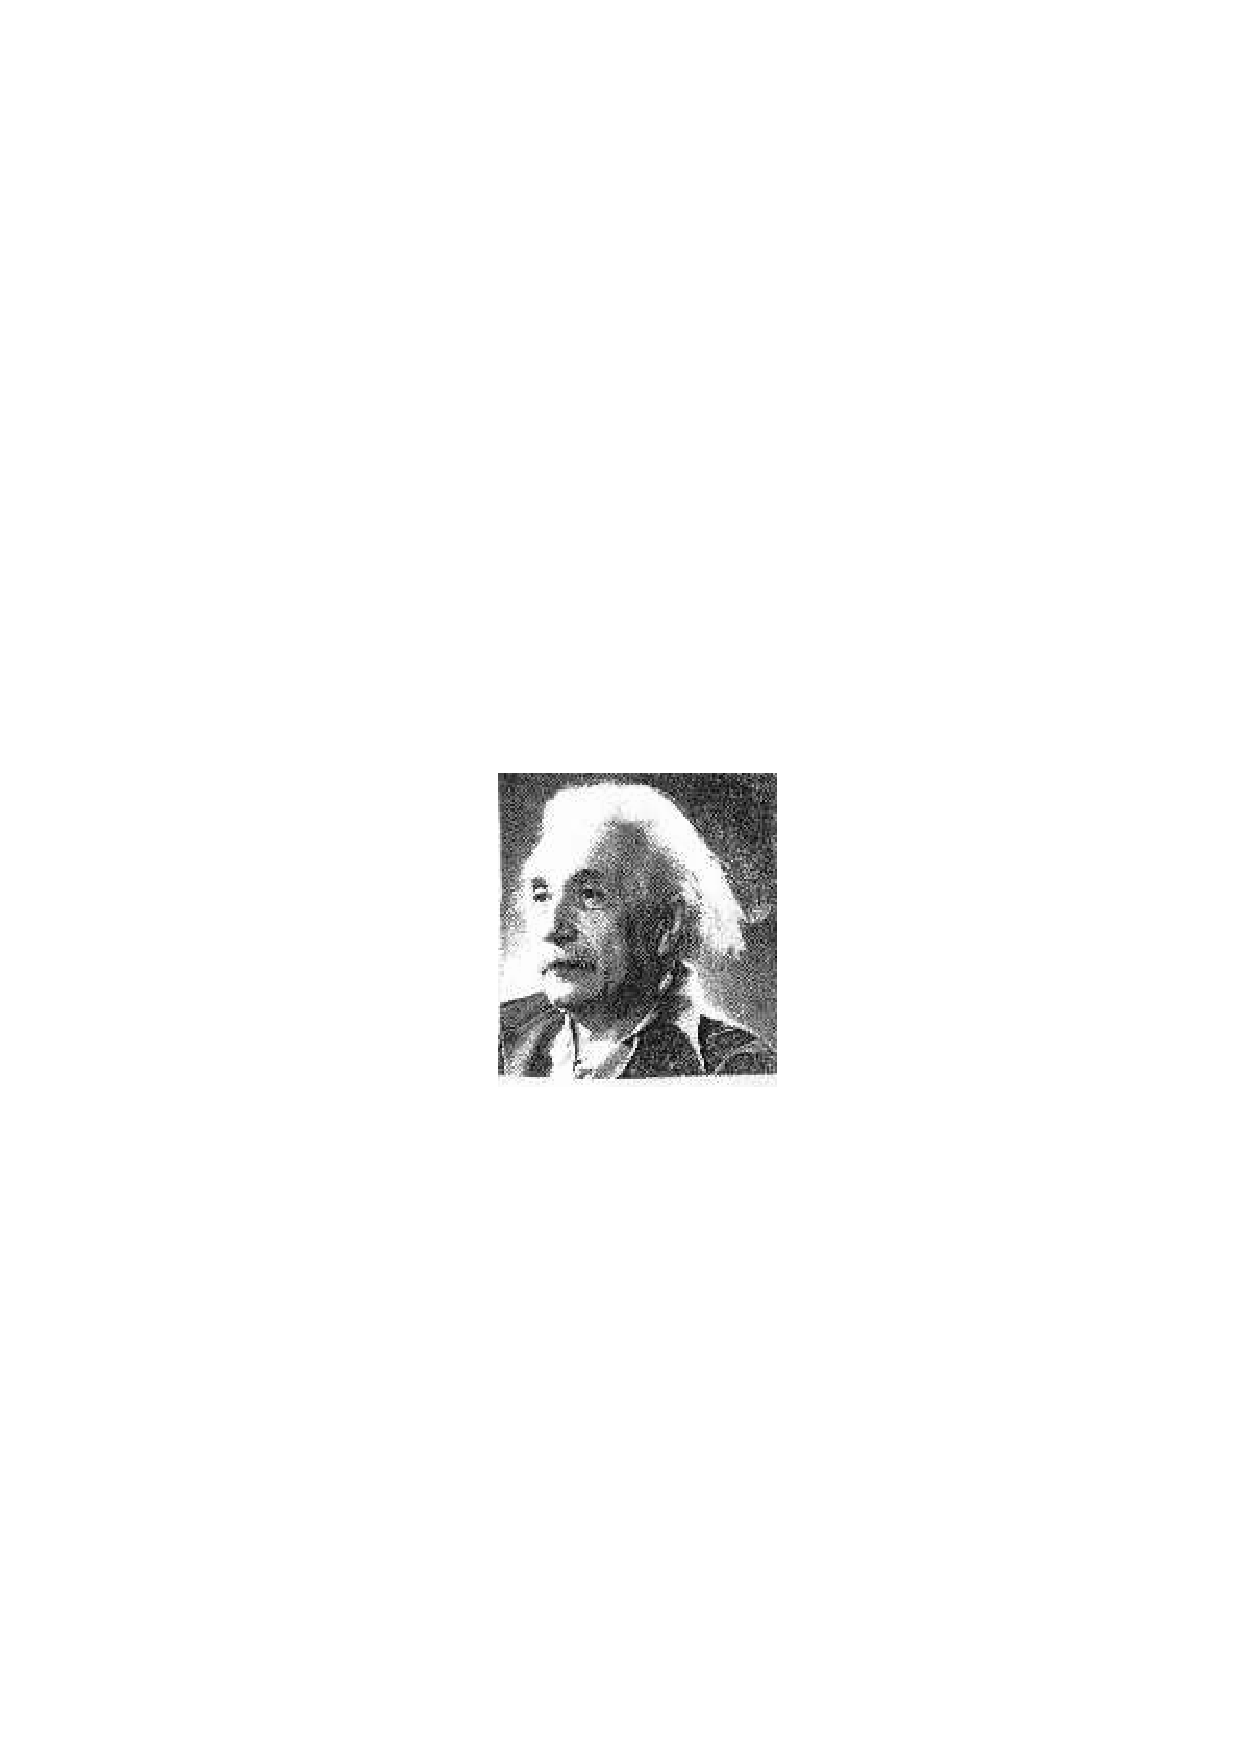
\includegraphics[width=3ex]{figsGeneric/Einstein.jpg}
\vspace{0ex}}
\hspace{0ex} 
}

\newcommand{\Einstein}{
\parbox{7mm}{\vspace{2mm}
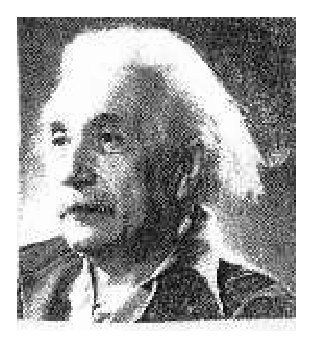
\includegraphics[width=10mm]{figsGeneric/Einstein.eps}
\vspace{-3mm}}\vspace{-3mm}
\hspace{2mm} 
}

\newcommand{\EinsteinLarge}{
\parbox{15mm}{\vspace{2mm}
\includegraphics[width=18mm]{figsGeneric/Einstein.eps}
\vspace{-2mm}}\vspace{-2mm}
\hspace{2mm} 
}



\providecommand{\EinsteinBeg}{
\vspace{-3mm}

\Einstein
\vspace{3mm}

}

\newcommand{\OK}{\ \includegraphics[width=1.2em]
   {$HOME/tex/inputs/figsGeneric/OK.png}}
\newcommand{\OKeps}{\includegraphics[width=1.2em]
   {$HOME/tex/inputs/figsGeneric/OK.eps}}
\newcommand{\contradiction}{
  \parbox{1.2em}{\vspace*{-0.2em}
  \includegraphics[width=0.9em, origin=br]
   {$HOME/tex/inputs/figsGeneric/contradiction.png}\vspace*{0.2em}}
}
\newcommand{\contradictioneps}{
  \parbox{1.2em}{\vspace*{-0.2em}
  \includegraphics[width=0.9em, origin=br]
   {$HOME/tex/inputs/figsGeneric/contradiction.eps}\vspace*{0.2em}}
}

\newcommand{\male}{\includegraphics[height=1em]
   {$HOME/tex/inputs/figsGeneric/male.eps}}
\newcommand{\female}{\includegraphics[height=1em]
   {$HOME/tex/inputs/figsGeneric/female.eps}}

\newcommand{\malepng}{\includegraphics[height=1em]
   {$HOME/tex/inputs/figsGeneric/male.png}}
\newcommand{\femalepng}{\includegraphics[height=1em]
   {$HOME/tex/inputs/figsGeneric/female.png}}

\newcommand{\circlei}{
  \parbox{1.2em}{\vspace*{-0.2em}
  \includegraphics[width=1.2em, origin=br]
   {$HOME/tex/inputs/figsGeneric/1circle.eps}\vspace*{0.2em}}
}

\newcommand{\circleii}{
  \parbox{1.2em}{\vspace*{-0.2em}
  \includegraphics[width=1.2em, origin=br]
   {$HOME/tex/inputs/figsGeneric/2circle.eps}\vspace*{0.2em}}
}

\newcommand{\circleiii}{
  \parbox{1.2em}{\vspace*{-0.2em}
  \includegraphics[width=1.2em, origin=br]
   {$HOME/tex/inputs/figsGeneric/3circle.eps}\vspace*{0.2em}}
}

\newcommand{\circleiv}{
  \parbox{1.2em}{\vspace*{-0.2em}
  \includegraphics[width=1.2em, origin=br]
   {$HOME/tex/inputs/figsGeneric/4circle.eps}\vspace*{0.2em}}
}

\newcommand{\circlev}{
  \parbox{1.2em}{\vspace*{-0.2em}
  \includegraphics[width=1.2em, origin=br]
   {$HOME/tex/inputs/figsGeneric/5circle.eps}\vspace*{0.2em}}
}


%******************************************************************
% General defs for tables
%******************************************************************

\providecommand{\titlebox}[1]{\parbox{140mm}{\vspace{2mm} #1 \vspace{2mm}}}

% top/bottom lines of the tables too close
\providecommand{\spacelinebot}[1]{\parbox[t]{1mm}{\hspace{1mm}\vspace{#1}}}
\providecommand{\spacelinetop}[1]{\parbox[b]{1mm}{\hspace{1mm}\vspace{#1}}}
\providecommand{\spacelinemid}[1]{\parbox[c]{1mm}{\hspace{1mm}\vspace{#1}}}
\providecommand{\spacingbot}{\parbox[t]{1mm}{\hspace{1mm}\vspace{3mm}}}
\providecommand{\spacingtop}{\parbox[b]{1mm}{\hspace{1mm}\vspace{6mm}}}
\providecommand{\spacingmid}{\parbox[c]{1mm}{\hspace{1mm}\vspace{9mm}}}



%******************************************************************
% General defs for figures                                        *
%******************************************************************

\providecommand{\icon}[1]{
  \parbox{7mm}{\vspace{2mm}
    \includegraphics[width=7mm]{#1}
    \vspace{-3mm}
  }
  \vspace{-3mm}
\hspace{1mm} }

% ex: \fig{0.9\textwidth}{epsfile}
\providecommand{\fig}[2]{
   \begin{center}
     \includegraphics[width=#1]{#2}
   \end{center}
}
\providecommand{\figSimple}[2]{
     \includegraphics[width=#1]{#2}
}

% ex: \figBox{0.9\textwidth}{epsfile}
% figure with parbox; necessary to make horizontal placement of figures/text
% without latex bugs
\providecommand{\figBox}[2]{
  \parbox{#1}{
     \begin{center}
     \includegraphics[width=#1]{#2}
    \end{center}
  }
}

% ex: \figBox{0.9\textwidth}{epsfile}{text}

\providecommand{\figBoxText}[3]{
  \parbox{#1}{
     \begin{center}
     \includegraphics[width=#1]{#2}
     \end{center}
     #3
  }
}

\providecommand{\oldfigc}[2]{
   \renewcommand{\baselinestretch}{1.0}
   \parbox[t]{#1}{\sloppy \small #2}
   \renewcommand{\baselinestretch}{\usualstretch}
   \small \normalsize
   }


% ex: \figps{110mm}{psfile}

\providecommand{\figps}[2]{
   \begin{minipage}[]{#1}
       \epsfxsize #1
       \epsffile{#2}
   \end{minipage}
   }

\providecommand{\figcaption}[3]{
   \renewcommand{\baselinestretch}{1.0} 
   \noindent
   \parbox[]{#1}
      {\sloppy \small Figure #2 \ 
       #3
       }
    \renewcommand{\baselinestretch}{\usualstretch}
    \small \normalsize
   }

% ex: \largefig{filename}{5mm}{\label}{captiontext}

\providecommand{\largefig}[4]{    % left fig, right text
   \begin{minipage}{\lenxtot}
       \figps{\lenxtot}{#1}
       \vspace{#2} \\
       \figcaption{\lenxtot}{#3}{#4}
   \end{minipage}
   }

% ex: \smallfig{\lenxa}{filename}{\lenxb}{\label}{captiontext}

\providecommand{\smallfig}[5]{    % left fig, right text
   \begin{minipage}{\lenxtot}
       \begin{minipage}{#1}
         \figps{#1}{#2}
       \end{minipage}
       \hfill
       \begin{minipage}{#3}
         \figcaption{#3}{#4}{#5}
       \end{minipage}
   \end{minipage}
   }


%******************************************************************
% General macros for math expressions                             *
%******************************************************************

\providecommand{\Int}{\int\limits}
\providecommand{\Sum}{\sum\limits}

\providecommand{\bfall}\textbf{\boldmath } % usual text AND math (after$)
\providecommand{\bfmath}[1]{\mbox{\textbf\boldmath{$#1$}}} % italics+fett!
\providecommand{\fett}\textbf{\boldmath } % usual text AND math (after$)

\providecommand{\dd}{{\textrm d}} %example \dd f/\dd x
\providecommand{\diff}[1]{ \ {\textrm d} #1 \, } % dx: differential operator d roman!
\providecommand{\dif}{\mathrm d} %example \dif f/\dif x
\providecommand{\e}{\mathrm e}   % example: \e^x
%!! Achtung: part, dp etc alles reservierte Befehle!!
\providecommand{\ablpart}[2]{\frac{\partial #1}{\partial #2}}  %d(#1)/d(#2)
\providecommand{\abl}[2]   {\frac{{\textrm d} #1}{{\textrm d} #2}}  % =\abltot
\providecommand{\abltot}[2]{\frac{{\textrm d} #1}{{\textrm d} #2}}  % d(#1)/d(#2)
\providecommand{\ablpartzwei}[2]{\frac{\partial^{2} #1}{\partial #2^{2}}} 
\providecommand{\ablparttwo}[2]{\frac{\partial^{2} #1}{\partial #2^{2}}} 
\providecommand{\ablpartmix}[3]{\frac{\partial^{2} #1}
           {\partial  #2 \ \partial #3}}
\providecommand{\ablpartmixed}[3]{\frac{\partial^{2} #1}
           {\partial  #2 \ \partial #3}}
\providecommand{\ablzwei}[2]{\frac{{\textrm d}^{2} #1}{{\textrm d} #2^{2}}} 

\providecommand{\cc}{^{\ast}}         %konj. komplex 
\providecommand{\complex}{C \hspace*{-0.65 em}
   \parbox{3mm}{\vspace*{-0.2 em} {\scriptsize /}}
    }
\providecommand{\cov}{\mbox{cov}}
\providecommand{\Cov}{\mbox{Cov}} %gross Cov!

\renewcommand{\d}[1]{\partial_{#1}}              %Diff.-operator
\providecommand{\deltat}{\mbox{$\delta(t-t')$}}
\providecommand{\deltar}{\mbox{$\delta(\v{r}-\v{r'})$}}
\providecommand{\deltax}{\mbox{$\delta(x-x')$}}
\providecommand{\deltavx}{\mbox{$\delta(\v{x}-\v{x}')$}}
\providecommand{\deltay}{\mbox{$\delta(y-y')$}}
\providecommand{\deltaz}{\mbox{$\delta(z-z')$}}
\providecommand{\deltart}{\mbox{$\delta(\v{r}-\v{r'})\delta(t-t')$}}
\providecommand{\deltaxyt}{\mbox{$\delta(x-x')\delta(y-y')\delta(t-t')$}}
\providecommand{\deltaij}{\mbox{$\delta_{ij}$}}
\providecommand{\deltaik}{\mbox{$\delta_{ik}$}}
\providecommand{\deltail}{\mbox{$\delta_{il}$}}
\providecommand{\deltajk}{\mbox{$\delta_{jk}$}}
\providecommand{\deltajl}{\mbox{$\delta_{jl}$}}
%arne klappt nicht:
%\providecommand{\dfrac}[2]{{\displaystyle \frac{#1}{#2}}}
\providecommand{\dsumi}{{\displaystyle \sum\limits_{i=1}^{n}}} %Summe im D-stil
\providecommand{\dint}[2]{{\displaystyle\int\limits_{#1}^{#2}}}
\providecommand{\dsum}[2]{{\displaystyle \sum\limits_{#1}^{#2}}}
\providecommand{\dsuml}[2]{{\displaystyle \sum\limits_{#1}^{#2}}} %Summe im D-stil
%\providecommand{\erw}[1]{\mbox{$\left \langle #1 \right \rangle$}} %Erwartungswert
\providecommand{\erw}[1]{\mbox{$E \left( #1 \right )$}} %Erwartungswert
\providecommand{\erf}[1]{\ \mbox{erf} \ #1} %Error function
\providecommand{\floor}[1]{{\textrm floor}\left(#1\right)}
\providecommand{\funkint}[1]{\int \!\!\cal{D}[#1]}
\providecommand{\hc}{^{\dagger}}         %konj. komplex 
\renewcommand{\Im}{\mbox{Im}}                  
\providecommand{\intd}[1]{\int \!d#1}
\providecommand{\intdn}[1]{\int \!\!d^{n}\v{#1}}
\providecommand{\intvol}{\int \!\!d^{3}} %keine Zahlen (d3) moegl.
\providecommand{\intvolr}{\int \!\!d^{3} r} %keine Zahlen (d3) moegl.
%\providecommand{\le}{\stackrel{<}{=}}   % less or equal
 
\providecommand{\nab}{\v{\nabla}}
\providecommand{\order}[1]{{\cal O}(#1)}
\providecommand{\overdot}[1]{\stackrel{.}{#1}}        
\renewcommand{\Re}{\mbox{Re}}                      
\providecommand{\re}{\mbox{Re}}                       
\providecommand{\rot}[1]{\v{\nabla}\times \v{#1}}
\providecommand{\sigeps}{\sigma_{\epsilon}}
\providecommand{\hatbeta}{\hat{\beta}}
\providecommand{\hatvec}[1]{\hat{\vec{#1}}}
\providecommand{\vecbeta}{\vec{\beta}}
\providecommand{\bfbeta}{\bfmath{\beta}}
\providecommand{\tilvecx}{\tilde{\vec{x}}}
\providecommand{\tilx}{\tilde{x}}
\providecommand{\hatvecbeta}{\hat{\vec{\beta}}}
\providecommand{\hatsigeps}{\hat{\sigma}_{\epsilon}}
\providecommand{\veceps}{\vec{\epsilon}}
\providecommand{\hatveceps}{\hat{\vec{\epsilon}}}
\providecommand{\hatsigy}{\hat{\sigma}_{y}}
\providecommand{\hatsig}{\hat{\sigma}}
\providecommand{\sumi}{\sum_{i=1}^n}
\renewcommand{\theta}{\vartheta} % zwei Arten von kleinen Thetas, ich
                                % will eins

\providecommand{\sub}[1]{dummy}
\providecommand{\sup}[1]{dummy}
% !! in some latex settings  \hspace{-0.8ex}, in some  \hspace{-0.0ex} right!
%\renewcommand{\sub}[1]{_{\text{{\scriptsize \hspace{-0.8ex}#1}}}}
%\renewcommand{\sup}[1]{^{\text{{\scriptsize \hspace{-0.8ex}#1}}}}
%\renewcommand{\sub}[1]{_{\text{{\scriptsize \hspace{-0.4ex}#1}}}}
%\renewcommand{\sup}[1]{^{\text{{\scriptsize \hspace{-0.4ex}#1}}}}
\renewcommand{\sub}[1]{_{\text{{\scriptsize \hspace{-0.0ex}#1}}}}
\renewcommand{\sup}[1]{^{\text{{\scriptsize \hspace{-0.0ex}#1}}}}
%\renewcommand{\sub}[1]{_{\rm \hspace{-0.0ex}#1}} %bug if \sub{\"OV} etc
%\renewcommand{\sup}[1]{^{\rm \hspace{-0.0ex}#1}}
%\providecommand{\tr}{^{\!\text{\scriptsize{T}}}}
\providecommand{\tr}{'}
\providecommand{\ueber}[2]{
  \left(\begin{array}{c}
     #1  \\ #2
  \end{array} \right)
}
\providecommand{\tilL}{\tilde{L}}



%\renewcommand{\vec}[1]{\mathbf{#1}}
\renewcommand{\vec}[1]{\text{\boldmath{$#1$}} }
\renewcommand{\bfmath}[1]{\text{\boldmath{$#1$}} }


%\renewcommand{\v}[1]{\mbox{\boldmath$#1$}}     %Vektor = fett
\renewcommand{\v}[1]{\vec{#1}}  %Vektorpfeil/fett je nach obigem renewcommand
%\renewcommand{\v}[1]{\bbox{#1}}     %Vektor = fett, revtex
%\renewcommand{\v}[1]{\underline{#1}} %Vektor = unterstrichen
\providecommand{\vscript}[1]{\mbox{{\scriptsize $\textbf #1$}}} % NOT for greek!


%\providecommand{\m}[1]{\underline{\v{#1}}}                  %Matrix
%\providecommand{\m}[1]{\underline{\underline{#1}}}           %Matrix
\providecommand{\m}[1]{\textbf{\textsf{#1}}\, } %Matrix=fett+gerade(nicht gr)
\providecommand{\mgr}[1]{\text{\boldmath {$#1$}}}  %Matrix griech. \sigma etc


\providecommand{\varabl}[2]{\frac{\delta #1}{\delta #2}}  %d(#1)/d(#2)

%******************************************************************
%      Independent vars etc.                                      *
%******************************************************************
 

\providecommand{\vonx} {\mbox{$(\v{x})$}}                   %(x)
\providecommand{\vonk} {\mbox{$(\v{k})$}}                   %(k)
\providecommand{\vonw} {\mbox{$(\omega )$}}                   %(omega)
\providecommand{\vonr} {\mbox{$(\v{r})$}}                   %(r)
\providecommand{\vonrs} {\mbox{$(\v{r'})$}}                   %(r')
\providecommand{\vonxyt} {\mbox{$(x,y,t)$}}                   %(x,y,z)
\providecommand{\vongrad} {\mbox{$(\v{\nabla })$}}            %(nabla)
\providecommand{\vonrgrad} {\mbox{$(\v{r},\v{\nabla })$}}     %(r,nabla)
\providecommand{\vonxt} {\mbox{$(\v{x},t)$}}                %(x,t)
\providecommand{\vonrt} {\mbox{$(\v{r},t)$}}                %(r,t)
\providecommand{\vonrsts} {\mbox{$(\v{r'},t')$}}                %(r',t')

%******************************************************************
% Misc.                                                           *
%******************************************************************
\providecommand{\nonu} {\nonumber}
\providecommand{\uu}[1]{\underline{\underline{#1}}} 
\providecommand{\COii}{\text{CO}$_2$}


%******************************************************************
% End general defs                                                *
%******************************************************************




%%% Local Variables: 
%%% mode: latex
%%% TeX-master: t
%%% End: 
%$
\usetheme{Dresden}

\usepackage[english]{babel}
%\usepackage{pgf,pgfarrows,pgfnodes,pgfautomata,pgfheaps,pgfshade, german, hyperref,etex,pictex}
\usepackage{pgf,pgfarrows,pgfnodes,pgfautomata,pgfheaps,pgfshade, hyperref,etex,pictex}
%\usepackage{dsfont, bm, amsmath,amssymb, epsfig, graphicx, marvosym,array,fancybox,}
\usepackage{dsfont, bm, amsmath,amssymb, epsfig, graphicx,array,fancybox,}
\usepackage[latin1]{inputenc}
\usepackage[all]{xy}       % \xymatrix

% color already defined in defsSkript, otherwise, define it here
%\definecolor{blueTUD}{rgb}{0.1,0,0.5} 

\setbeamertemplate{frametitle}[default][center]
\setbeamerfont{frametitle}{size=\large,series=\bfseries}
%\setbeamercolor{frametitle}{blueTUD}
\setbeamercolor{frametitle}{fg=blueTUD} % {fg=red,bg=yellow}

\author{Martin Treiber}
\title{Econometrics Master's Course: Methods}
\institute{OSV}

\selectlanguage{english}
\renewcommand{\baselinestretch}{1}

\beamertemplateshadingbackground{white!10}{white!10}
\beamertemplatetransparentcovereddynamic
\newfont{\tabfont}{cmr7 at 7pt}
\renewcommand{\arraystretch}{1}
\colorlet{alert}{blue!60!black} \colorlet{beameralert}{alert}

\geometry{left=1cm, right=0.5cm}

\def\colorize<#1>{%
  \temporal<#1>{\color{structure}}{\color{black}}{\color{black}}}

\graphicspath{{./figures/}}

\input{cyracc.def}

\newcommand{\frameofframes}{/}
\newcommand{\setframeofframes}[1]{\renewcommand{\frameofframes}{#1}}

\setframeofframes{of}
\makeatletter

\setbeamertemplate{headline}
{
    \begin{beamercolorbox}[ht=3ex,dp=1.125ex, leftskip=.3cm,rightskip=.3cm plus1fil]{title in head/foot}%
        \includegraphics[scale = 0.08]{TULogoWeiss.png}
        \hspace{0.3cm}
        {\usebeamerfont{title in head/foot}\insertshorttitle}%
        \hfill%
        {\usebeamerfont{section}\usebeamercolor[fg]{section}\insertsection}
        \hfill%
        {\usebeamerfont{subsection}\usebeamercolor[fg]{subsection}\insertsubsectionhead}
    \end{beamercolorbox}
}


\setbeamertemplate{footline}{
%    \begin{beamercolorbox}[ht=2.5ex,dp=1.125ex,leftskip=.3cm,rightskip=.3cm plus1fil]{title in head/foot}%
%        {\usebeamerfont{author}\insertshortauthor}%
%        \hfill%
%        {\usebeamerfont{frame number}\usebeamercolor[fg]{frame number}\insertframenumber~\frameofframes~\inserttotalframenumber}
%    \end{beamercolorbox}
}

\newenvironment{beispiel}%
{{\color{mygreen}\textbf{Beispiel:} }\color{mygreen}}%
{}%

\newenvironment{beispiele}%
{{\color{mygreen}\textbf{Beispiele:} }\color{mygreen}}%
{}%


%$
%\input{../style/defs}
\usepackage{graphicx}

\newcommand{\pathDiscrChoice}{$HOME/vorlesungen/Verkehrsoekonometrie_Ma/discrChoice_cc_Levmar} %$

%##############################################################

\begin{document}

\section{4. Discrete-Choice Theory}

%##############################################################
\frame{\frametitle{Chapter 4. Discrete-Choice Theory and Models}
%##############################################################
\bi
\item 4.1. The nature of discrete decisions
\item 4.2. Basic concepts: alternatives, utilities, Homo Oeconomicus
\item 4.3. Deterministic utilities and how to model them
\item 4.4. Random utilities and choice probabilities
\item 4.5. Logit models
\item 4.6. Probit models
\item 4.7. Elasticities
\item 4.8. Maximum-likelihood estimation
\item 4.9. Estimation errors and Fisher's information matrix
\item 4.10. Significance tests
\item 4.11. Goodness-of fit measures
\item 4.12. Parameter nonlinear models
\item 4.13. GEV and Nested-Logit models
\item 4.14. Mixed-Logit models
\item 4.15. Models for Reliability
\ei
}

\subsection{4.1. The nature of discrete decisions}

%##############################################################
\frame{\frametitle{4.1. Introduction: The nature of discrete decisions}
%##############################################################
\centering{Example: the four-step model of transportation planning}
\fig{1.0\textwidth}{figsDiscr/vierstufenmodellDiscr_eng.png}
}

\subsection{4.2. Basic concepts}

%##############################################################
\frame{\frametitle{4.2. Alternatives and how to model them}
\bi
\item Each person (or choice set) $n$ has a certain set of discrete
  alternatives: 
  ${\cal A}_n=\{a_{ni}\}$ containing alternatives $i=1, ..., I_n$
\pause \item The number $I_n$ of alternatives is finite and should not be too large
\pause \item The alternative set needs to be \bfdef{exclusive}
  (non-cumulative), i.e., a 
  person can chose at most one alternative
\pause \item The set must be \bfdef{complete}, i.e., at least one
  alternative must be chosen. Complete and exclusive $\Rightarrow$ exactly one alternative
  chosen
\pause \item The alternatives need to be sufficiently different from each other.
\ei
{\small
\pause \bfAsk{?} What to do if a person has the option to
not select anything?

\pause \bfAsk{?} What to do if multi-modal trips (e.g., bike+tram) are possible?

\pause \bfAsk{?} Assume that someone  has no
car or bike available. How to model the four alternatives 
ped, bike, car, PT for this person? Give two possible solutions

\pause \bfAsk{?} Explain ``sufficiently different alternatives'' by red and
blue buses.

\pause \bfAsk{?} What to do with continuous alternatives such as desired speed?
}
}


%##############################################################
\frame{\frametitle{4.2. The essence of the Homo Oeconomicus:\\two alternatives}
%##############################################################
\fig{0.7\textwidth}{figsDiscr/zweiAlternat-U_eng.png}
Each red point corresponds to a given situation at a given time
\bdm
\text{Alternative } i\sub{selected}=\text{arg} \max_i U_i
\edm
}


%##############################################################
\frame{\frametitle{Decisions under uncertainty}
%##############################################################

\fig{0.95\textwidth}{figsDiscr/zweiAlternat-P_eng.png}

\bdm
\text{Alternative } i\sub{selected}=\text{arg} \max_i U_i
= \text{arg} \max_i V_i+\epsilon_i
\edm

\bi
\item On an individual level, the decision is ``yes''
  (1) or ``no'' (0)
\item On an aggregated level, we have a certain
  probability between  0 and 1.
\ei
}

%##############################################################
\frame{\frametitle{Structure and classification of dicrete-choice models}
%##############################################################
\fig{1.0\textwidth}{figsDiscr/discrKomp_eng.png}
}


\subsection{4.3. Deterministic utilities}


%##############################################################
\frame{\frametitle{4.3. Modeling deterministic utilities}
%##############################################################
\bi
\item Basically, the deterministic utilities $V_{ni}$ of alternative
  $i$ for person $n$ are like the endogenous
variables of regression models: continuous and made up of linear
factors:
\bdm
V_{ni}=\sum_m \beta_{m} X_{mni}
\edm
\vspace{-0.8em}

\pause \item The person index (or choice-set index) $n$ plays the role of a
  data-point index $i$ in regression models (the index naming is by
  convention) and $X_{mni}$ corresponds to the system matrix.
\\[1em]

\pause \item The factors contain alternative-specific constants and
exogeous variables of one of the following three categories: 
\bi
\item \bfdef{alternative-specific constants (ACs)}
  play the role of constants in regression models,
\item \bfdef{characteristics} are attributes of the alternatives,
\item \bfdef{socioeconomic factors} are attributes of the decision makers,
\item \bfdef{external factors} depend neither on the alternatives nor the
  persons but influence the decisions.
\ei


\ei
}


%##############################################################
\frame{\frametitle{Factors I: Alternative-specific constants (ACs)}
%##############################################################
\bi
\item In most situations, there are systematic (``ad-hoc'')
  preferences for certain 
  alternatives not 
  explained by the characteristics or socioeconomic variables.
\pause \item Since the choice depend on utility
  \emph{differences}, only, normal constants are of no use. We need
  \bfdef{alternative-specific constants} or \bfdef{ACs} which are
  essentially \emph{selector dummy variables}: 
\bdm
V_{ni}=\beta_{01}\delta_{1i}+...+\beta_{0,I-1}\delta_{I-1,i},\quad
\delta_{ji}=\twoCases{1}{i=j}{0}{i\neq j}
\edm
\pause \item The parameter $\beta_{0i}$ denotes the \bfdef{ad-hoc
  preference}  of Alternative
  $i$ (in utility units) over 
the reference alternative $I$ if all other factors $X_{mni}=0$.
\ei
\pause \bfAsk{?} What would happen if using a normal constant, $V_{ni}=\beta_0$? 

\pause \bfAsk{?} Give the ad-hoc preference of alternative $j$ over $i$, 
$i \neq I$.

\pause \bfAsk{?} What changes when making Alternative 1 the
reference? 

}

%##############################################################
\frame{\frametitle{Factors II: Characteristics}
%##############################################################
\bi
\item The characteristic $C_{mni}$ is the $m\sup{th}$ attribute of
  alternative $i$ for person (choice set) $n$.

\pause \item Examples: 
\bi
\item Complex travel time $C_{1in}=T_{ni}$ for person $n$ when
  travelling by transport mode $i$,
\item Ad-hoc costs $C_{2in}=C_{ni}$ for person $n$ when using mode $i$
\ei

\pause \item Characteristics can be identified directly with factors,
$X_{mni}=C_{mni}$. Modelling variants:
\bi
\item \bfdef{generic} ansatz
  $V_{ni}=...+\beta_mC_{mni}$  (the same parameter $\beta_m$ for all alternatives $i$),
\item \bfdef{alternative-specific} ansatz
  $V_{ni}=...+\beta_{mi}C_{mni}$ with
  alternative-specific parameters $\beta_{mi}$.
\ei
\ei

\pause
\bfAsk{?} Which way is to be preferred when modelling (i) travel times and
(ii) costs? (justify!)

\bfAsk{?} Give an example of a characteristic not depending
 on the person. %\tiny{Reliability of a mode}
 
}


%##############################################################
\frame{\frametitle{Factors III: Socio-economic variables}
%##############################################################
\bi
\item The socioeconomic variable $S_{mn}$ denotes the $m\sup{th}$
  attribute of person $n$, e.g., age, gender, income, or
  the distance to the next PT station.
\pause \item Since, by definition, socio-economic variables do \emph{not}
  depend on the alternative and the choice depend on utility
  \emph{differences}, only, they cannot identified directly by a
  factor.
\pause \item Instead, there are two ways to specify valid linear factors: 
\benum
\item Formulate in an alternative-specific way with ACs:
\bdm
V_{ni}=...+\beta_{m1}S_{mn}\delta_{1i}+...+\beta_{m,I-1}S_{mn}\delta_{I-1,i},\quad
\delta_{ji}=\twoCases{1}{i=j}{0}{i\neq j}
\edm
\item Combine with a characteristic $m'$, e.g.,
  $X_{mni}=S_{mn}C_{m'ni}$ and model it in an alternative-specific way
  $V_{ni}= ... + \beta_{mi}S_{mn}C_{m'ni}$
\eenum
\ei

\pause \bfAsk{?} What would happen when setting
$V_{ni}=...+\beta_mS_{mn}$ for all $i$? 

\pause \bfAsk{?} How to model that woman prefer PT over bikes more than men?

\pause \bfAsk{?} How to model an income-dependent time sensitivity?

\pause \bfAsk{?} Why it is not possible to use the age directly?
}


%##############################################################
\frame{\frametitle{Factors IV: External variables}
%##############################################################
\bi
\item External variables influence the decisions although they neither
  depend on the alternatives nor the persons, e.g., the weather with
  the dummy $W=0$
  (no rain) or $W=1$ (rain).
\pause \item The specification depends on the way they influence decisions:
\bi
\item Affecting the alternatives directly: $X_{mni}=W\delta_{mi}$,
\item affecting the \emph{alternatives} indirectly via a characteristic
  $m'$, e.g. travel time:  $X_{mni}=WC_{m'ni}$,
\item affecting the \emph{decision maker} via a socioeconomic
  attribute $m'$, e.g., the gender:
   $X_{mni}=WS_{m'n}\delta_{mi}$,
\item combinations thereof.
\ei
\ei

\pause 

{\small
\bfAsk{?} Assume there are three modes bike, PT and car and define
$W=0$ (not snowing) and $W=1$ (snowing). Model the effect of snow on
the decision making in following situations:
\vspace{-0.5ex}

\bi
\item[\bfAsk{?}] The car becomes less attractive because I need to shovel off the snow
\pause \item[\bfAsk{?}] The bike is protected in a shed but driving becomes
  less attractive because the road is slippery 
  and it's cold
\pause \item[\bfAsk{?}] Woman dislike biking even more than men when it's snowing
\ei
}
}

%##############################################################
\frame{\frametitle{Wrap up: modelling a certain choice situation}
%##############################################################

{\small
Given is a SP survey for mode choice with three
alternatives 
\bi
\item $i=1$: pedestrian mode: door-to-door travel time $T_1$
\vspace{-0.5em}

\item $i=2$: bicycle: door-to-door travel time $T_2$
\vspace{-0.5em}

\item $i=3$: motorized: door-to-door travel time $T_3$, ad-hoc costs
  $C_3$
\ei

Furthermore, we distinguish the gender of the deciding person ($g=0$:
male; $g=1$: female) and the weather ($W=0$: good; $W=1$: bad).
\bi
\item[\bfAsk{?}] Specify a model for generic time and
  cost sensitivities making $i=3$ the reference. Give the meaning and
  expected signs of
  the parameters. 
\pause \item[\bfAsk{?}] Now, formulate the travel time dependence
  alternative-specifically.
\pause \item[\bfAsk{?}] Include the weather dependence assuming that the
  motorized mode is favoured in bad weather proportionally to the travel time.
\pause \item[\bfAsk{?}] Now assume that women give the motorized modes a
  fixed ``bonus'' compared to men and that they also are more sensitive to
  the weather.
\pause \item[\bfAsk{?}] Which parameters would change in which way (i) if $W=1$
  stands for good instead of bad weather; (ii) if $g=1$ stands for
  men instead of woman; (iii) if the reference alternative is $i=1$
  instead of $i=3$?
\ei
}

}

\subsection{4.4. Random utilities and choice probabilities}

%##############################################################
\frame{\frametitle{4.4. Random utilities: where do the come from?}
%##############################################################

\bi
\item Not all relevant characteristics $\vec{C}$ and socioeconomic
  variables $\vec{S}$ are included:
\bdm
U_i=U(\underbrace{\vec{C}_i, \vec{S}}_\textrm{known}, 
          \underbrace{\vec{C}'_i, \vec{S}'}_\textrm{unknown})
  =V(\vec{C}_i, \vec{S})+ \epsilon^{(1)}_i.
\edm
\red{whatch out} for neglected systematic influences leading to a bias

\pause \item Measuring/observation errors
\bdm
U_i=U(\vec{C}_i \underbrace{+\vec{\epsilon}_i}_\textrm{measuring\ error}, 
  \vec{S} \underbrace{+\vec{\epsilon}}_\textrm{measuring\ error})
  =V(\vec{C}_i, \vec{S}) + \epsilon^{(2)}_i.
\edm

\pause \item Relevant variables are only indirectly observable via
  \bfdef{instrument variables} such as the address $S'$ of one's home for
  the income $S$:
\bdm
U_i=U(\vec{C}_i, \vec{S})
  =V(\vec{C'}_i, \vec{S}')+ \epsilon^{(3)}_i.
\edm


\pause \item True irrationality $\epsilon^{(4)}_i$.
\ei
}



%##############################################################
\frame{\frametitle{Choice probabilities}
%##############################################################

\bi
\item The three basic components of discrete-choice models are
  \bfdef{determinstic (explained)
utilities} $V_i$, \bfdef{random utilities (RUs)} $\epsilon_i$, and a decision
rule based on the 
\bfdef{Homo Oeconomicus}:

\maindm{i\sub{selected}=\text{arg} \max_i U_i
= \text{arg} \max_i (V_i+\epsilon_i)}
\vspace{0.5em}

\pause\item By virtue of the RUs, this microscopically fixed decision
rule leads 
to \bfdef{choice probabilities} $P_i$ when aggregating over many
decisions. 
\ei
\vspace{0.5em}

\pause
$\begin{array}{rcl}
\text{\emph{Binomial case: \quad }}P_1 &=& \text{Prob}(U_1 \ge U_2)\\
    &=& \text{Prob}(V_1+\epsilon_1\ge V_2+\epsilon_2)\\
    &=& \text{Prob}(\epsilon_2-\epsilon_1\le V_1-V_2)\\
    &=& F_{\epsilon_2-\epsilon_1}(V_1-V_2).
\end{array}$
%$
\vspace{1em}

\pause \bfAsk{?} What does this result mean in words?

\pause \bfAsk{?} Derive explicit formulas for 
$\epsilon_i \sim$ i.i.d $U(-1,1)$
and $\epsilon_i \sim $ i.i.d $N(0,1)$

\pause \bfAsk{?} What would happen for \unit[100]{\%} crrelated RUs?
}


%##############################################################
\frame{\frametitle{Translation and scale invariance}
%##############################################################

The general choice formula $i\sub{selected}=\text{arg} \max_i
(V_i+\epsilon_i)$ leads to two far-reaching consequences:
\bi
\item \bfdef{Translation invariance}: 
\maindm{V_1+\epsilon_1>V_2+\epsilon_2 \Longleftrightarrow 
V_1+\epsilon_1+c>V_2+\epsilon_2+c, \quad c \in I\!\!R}
 
\bi
\item Only differences matter. In particular, one can set one
  deterministic utility $V_{i'}=0$  making $i'$ the reference alternative.
\item Nonzero expectation values $E(\epsilon_i)$ (as in
  Logit models) are irrelevant.
\ei

\pause \item \bfdef{Scale invariance}: 
\maindm{V_1+\epsilon_1>V_2+\epsilon_2 \Longleftrightarrow 
\lambda(V_1+\epsilon_1)>\lambda(V_2+\epsilon_2), \quad \lambda>0}

\bi
\item A \emph{simultaneous} scaling of all $V_i$ and $\epsilon$ leaves
  the choice unchanged (one could even apply a strictly monotonously
  increasing 
  function defined in $I\!\!R$ such as $\exp(.)$ to all $V_i+\epsilon_i$)
\item One can normalize $\epsilon_i$ without loss of generality.
In any case, $V_i$ is given in multiples of the standard deviation of
  $\epsilon_i$
\ei
\ei


}

 
\subsection{4.5. Logit models}

%##############################################################
\frame{\frametitle{4.5. Logit model: Definition}
%##############################################################

All Logit models are defined by
\bfdef{Gumbel-distributed} random utilities. 
\vspace{0.5em}

\bi
\item 
The most widely used \bfdef{Multinomial-Logit model} has RUs
  distributed according to
\maindmIntext{
\epsilon_i \sim \text{i.i.d Gumbel}(0,1)
}
\vspace{1em}
{\small
\pause \item Distribution:
\bdm
F\sub{Gu}^{(\eta,\lambda)}(x)=\exp \left[-e^{-\lambda(x-\eta)}\right]
\edm

\pause \item Density:
\bdm
\label{fGumbel}
f\sub{Gu}^{(\eta,\lambda)}(x)
=\abl{F\sub{Gu}^{(\eta,\lambda)}(x)}{x}
=\lambda e^{-\lambda(x-\eta)}
\exp \left[-e^{-\lambda(x-\eta)}\right].
\edm

\pause \item Statistical properties:
\bdm
\epsilon\sub{mode}=\eta, \quad 
E(\epsilon)=\eta+\gamma/\lambda \ \text{with} \ \gamma=0.5772, \quad 
V(\epsilon)=\frac{\pi^2}{6\lambda^2}
\edm
}
\vspace{-0.5em}

\pause \item The numerical values of $V_i$ are about
$\pi/\sqrt{6}\approx 1.28$ times as large as if $V(\epsilon)$ were $=1$
(\bfAsk{why?})  
\item The nonzero  $E(\epsilon_i)=0.5772$ is
  irrelevant (\bfAsk{why?}) 
\ei

}



%##############################################################
\frame{\frametitle{Density functions of some Gumbel distributions}
%##############################################################
\fig{0.9\textwidth}{figsDiscr/gumbel_f.png}

}

%##############################################################
\frame{\frametitle{Gumbel distribution as a limit distribution for max(.)}
%##############################################################
\placebox[center]{0.50}{0.71}
{\parbox{0.95\textwidth}{{\small
 The maximum of many i.i.d. random variables $X_i$ with exponential
tails $\propto \exp(-\lambda x)$ approaches a Gumbel or Generalized Extreme Value Type-I
distribution: \\[-1em]
\bdm
\max(X_1, ..., X_n) \stackrel{\text{asympt.}}{\sim} 
\text{Gu}(\ln n, \lambda)
\edm
\\[-0.9em]
\emph{Example 1}: Maximum of i.i.d. exponentially distributed RUs
}}}


\placebox[center]{0.25}{0.36}
{\figSimple{0.55\textwidth}{figsDiscr/gumbelGrenz_f.png}}

\placebox[center]{0.28}{0.10}
{\parbox{0.50\textwidth}{{\small
Densities of the maximum of 1, 2, 20, and 100 i.i.d. random variables
}}}


\placebox[center]{0.75}{0.36}
{\figSimple{0.55\textwidth}{figsDiscr/gumbelGrenz_F.png}}

\placebox[center]{0.78}{0.10}
{\parbox{0.45\textwidth}{{\small
Corresponding distribution\\ functions
}}}

}


%##############################################################
\frame{\frametitle{Gumbel distribution as a limit distribution for max(.)}
%##############################################################

\placebox[center]{0.50}{0.80}
{\emph{Example 2}: Maximum of i.i.d. combined uniform-exponential RUs}

\placebox[center]{0.25}{0.53}
{\figSimple{0.55\textwidth}{figsDiscr/gumbelGrenz2_f.png}}

\placebox[center]{0.28}{0.25}
{\parbox{0.50\textwidth}{\small
Densities of the maximum of 1, 2, 20, and 100 i.i.d. random variables}
}


\placebox[center]{0.75}{0.53}
{\figSimple{0.55\textwidth}{figsDiscr/gumbelGrenz2_F.png}}

\placebox[center]{0.78}{0.25}
{\parbox{0.45\textwidth}{\small Corresponding distribution\\ functions}}

\placebox[center]{0.50}{0.11}
{\parbox{1.0\textwidth}{
\bfAsk{?} Give reasons why the maximum of two independent Gumbel
distributed random variables of the same scale parameter is Gumbel
distributed as well}}

}

%##############################################################
\frame{\frametitle{Properties of the Multinomial-Logit Model (MNL)}
%##############################################################

\bi
\item Models of the Logit family (MNL, nested Logit, GEV models) 
are the only ones with explicit
  expressions for the choice probabilities for the multinomial case
  $I>2$. For the MNL itself, we have

\maindm{P_i\sup{MNL}=\frac{\exp(V_i)}{\sum_j \exp(V_j)}}
 
\vspace{1em}

\pause \item Besides the translational and scale invariance of all simple
  discrete-choice models, the MNL has the \bfdef{Independence of
    Irrelevant Alternatives (IIA)} property: 

\maintextbox{0.75\textwidth}{IIA property: The relative preference
 of Alternative $i$ over $j$ as defined by the choice probability ratio
 $P_i/P_j$ does not depend on other alternatives $k \neq i,j$}
\ei
}


%##############################################################
\frame{\frametitle{Alternative definition for the MNL}
%##############################################################

\bi
\item
The IIA property is exclusively true for the MNL. In fact, the
  MNL can be equivalently defined by the IIA property instead of
  i.i.d. Gumbel RUs.
\vspace{1em}

{\small
\pause \item[\bfAsk{?}] Show that the MNL choice probabilities satisfy
  translational invariance.\\[1ex]
\pause \item[\bfAsk{?}] For a comparison with another model, we want
  $V(\epsilon_i)=1$ 
  instead of $\pi^2/6$. In which way the model parameters must be
  changed?\\[1ex] 
\pause \item[\bfAsk{?}] Derive the IIA property from the choice probability
  formula.\\[1ex] 

\pause \item[\bfAsk{?}] The choice probabilities of three alternatives are given by
$P_1=0.2$, $P_2=0.4$, and $P_3=0.4$. Now, Alternative~3 is no longer
available. Give the new Logit choice probabilities.\\[1ex]

\pause \item[\bfAsk{?}] The Gumbel distribution is the limit distribution
  of the maximum of exponentially-tailed random variables. Is there really a 
  justification for this sort of distribution if the
  RUs are the result of many unknown/not considered effects?
}
\ei

}



\subsection{4.6. Probit Models}

%##############################################################
\frame{\frametitle{4.6. Probit Models}
%##############################################################

The \bfdef{Probit Model} class is defined by (generally correlated)
Gaussian RUs.

\bi
\item The general multinomial Probit model (MNP) has random utilities
\maindmIntext{\veceps \sim N(\vec{0}, \vec{\Sigma})} with the
variance-covariance matrix $\vec{\Sigma}$ of the RUs
\pause \item The special case of the i.i.d. MNP with $\vec{\Sigma}=\m{1}$
  (unit matrix) or
  $\epsilon_i \sim  \text{i.i.d. }N(0,1)$ has similar
  properties as the MNL. However, for $I\ge 3$, the MNP needs a
  onedimensional integral to calculate the choice probabilities.
\pause \item Often, i.i.d Gaussian RUs can be motivited by the central-limit
  theorem while Gumbel distributed ones cannot. However, since the MNL behaves similarly and has explicit
  choice probabilities and a simpler calibration, it is often favoured
  over the i.i.d. MNP.
\pause \item[\bfAsk{?}] Why one can set the variance-covariance matrix to be
  the unit matrix (i.e. setting all variances=1) in case of the i.i.d MNP?
\ei
}

%##############################################################
\frame{\frametitle{Choice probabilities of the binary Probit model I}
%##############################################################

\bi
\item Binary i.i.d. Probit: 
\maindm{
\epsilon_i \sim \text{i.i.d. }N(0,1)
}
\vspace{1em}

\pause\item Choice probabilities: 
\vspace{1em}
\maindm{
P_1=\Phi\left(\frac{V_1-V_2}{\sqrt{2}}\right), \quad P_2=1-P_1
}
\vspace{1em}

{\small
\pause\item [\bfAsk{?}] Derive the choice probabilities from the general
  binary formula. \emph{Hints:} (i)
  a linear combination of  Gaussians is
  again a Gaussian, (ii) use the general rules ($a, b \in I\!\!R$ and
  $X_1, X_2$ random variables) 
\bdma
E(aX_1+bX_2) &=& aE(X_1)+bE(X_2), \\
V(aX_1+bX_2) &=& a^2V(X_1)+b^2V(X_2)+2ab\, \text{Cov}(X_1,X_2)
\edma

\pause\item [\bfAsk{?}] The Logit time and cost sensitivities are $\hatbeta_T=\unit[-0.1]{min^{-1}}$ and 
$\hatbeta_C=\unit[-0.6]{\text{\euro}^{-1}}$. Give the implied value of
time (VOT) and the approx. parameter values and VOT for the
corresponding Probit model.
}
\ei
}

%##############################################################
\frame{\frametitle{Choice probabilities of the binary Probit model II}
%##############################################################
\placebox[center]{0.24}{0.62}
{\figSimple{0.55\textwidth}{figsDiscr/fGauss.png}}

\placebox[center]{0.27}{0.25}
{\parbox{0.45\textwidth}{
Densities of the \blue{standardnormal distributed
      random utilities $\epsilon_1$ and $\epsilon_2$} and of the
\red{utility difference $\epsilon_1-\epsilon_2$}
}}


\placebox[center]{0.74}{0.62}
{\figSimple{0.55\textwidth}{figsDiscr/binProbit_P1.png}}


\placebox[center]{0.77}{0.25}
{\parbox{0.45\textwidth}{
Distribution functions of the \blue{random utilities} and the
\red{utility difference} as a function of the deterministic utility
difference  $V_1-V_2$
}}

}







%##############################################################
\frame{\frametitle{Choice probabilities of trinomial i.i.d. Probit
    and Logit}
%##############################################################

\placebox[center]{0.25}{0.52}
{\figSimple{0.60\textwidth}{figsDiscr/pProbitTrinom_V1V2.png}}

\placebox[center]{0.72}{0.52}
{\figSimple{0.60\textwidth}{figsDiscr/pLogitTrinom_V1V2.png}}

\placebox[center]{0.20}{0.14}
{Symmetrie considerations:}
\placebox[center]{0.67}{0.14}
{\parbox{0.6\textwidth}{\small
\bdma
P_2(V_2-V_3, V_1-V_3) &=& P_1(V_1-V_3,V_2-V_3),\\
P_3(V_2-V_3, V_1-V_3) &=& 1-P_1-P_2
\edma}}

}



\subsection{4.7. Elasticities}

%###################################################
\frame{\frametitle{4.7. Elasticities}
%###################################################

{\small
\bi
\item
\emph{General definition:}
\maintextbox{0.8\textwidth}
{Elasticities denote the percentaged change of endogenous
  variables $y_i$ per small percentaged change of exogenous variables
  $x_j$ for an average situation
\vspace{-1em}
\bdm
\epsilon_{ij}=\frac{\bar{x}_j}{\bar{y}_i}
\left.\ablpart{y_i}{x_j}\right|_{\vec{x}=\bar{\vec{x}},\vec{y}=\bar{\vec{y}}}
\edm 
\vspace{-1em}
}


\pause \item \emph{Regression:} 
\vspace{-2em}
\bdm
y=\sum_j\beta_jx_j+\epsilon, \quad
\epsilon_j=\frac{\bar{x}_j}{\bar{y}}\ablpart{y}{x_j}
=\frac{\bar{x}_j}{\bar{y}} \, \hatbeta_j
\edm

\pause \item \emph{Discrete-choice models:} 

Generally, with several endogenous variables,  one distinguishes between
\bi
\item \bfdef{Substitution} vs, \bfdef{full/ordinary} elastities,
\item \bfdef{Microscopic} vs, \bfdef{macroscopic} elastities,
\item \bfdef{proper elasticity} vs. \bfdef{cross-elasticity}
\ei

\pause \item[\bfAsk{?}] Why there are only substitution elastities in
discrete-choice models? 

\ei
}
}

%###################################################
\frame{\frametitle{Microscopic Logit elasticities}
%###################################################
Since elasticities describe macroscopic aspects, we take the
choice probabilities $P_i$ rather than the discrete actual choices as
endogenous 
variables. For the general deterministic utilities
\bdm
V_{ni}=\sum_m\beta_{mi}{x_{mni}}
\edm
\vspace{-2em}

we derive the
{\small
\bi
\item \bfdef{Proper (substitution) elasticities:} The attribute
  (characteristic) $m$ of an alternative $i$ feeds back on the demand
  for this alternative:
\maindm{\epsilon_{nii}\sup{(mic,m)}=
\frac{x_{mni}}{P_{ni}}\ablpart{P_{ni}}{x_{mni}}
=\beta_mx_{mni}(1-P_{ni})
}
\pause\item \bfdef{Cross elasticities:} The attribute
  (characteristic) $m$ of an alternative $j$ feeds back on the demand
  for another alternative $i\neq j$:
\maindm{\epsilon_{nij}\sup{(mic,m)}=
\frac{x_{nmj}}{P_{ni}}\ablpart{P_{ni}}{x_{nmj}}
=-\beta_mx_{nmj}P_{nj}
}
\ei
}

}

%###################################################
\frame{\frametitle{Some questions on micro-elasticities}
%###################################################

\bi
\item[\bfAsk{?}] Derive the formulas for the proper and cross
  elasticities from the expression for $V_{ni}$ and the Logit
  probabilities

\pause \item[\bfAsk{?}] Derive and motivate the ``null sum'' condition
  $\sum_i P_{ni}\epsilon_{nij}^m=0$ 

\pause \item[\bfAsk{?}] The cross elasticities do not depend on
  $i$, i.e., on the target alternative for the changing
  demand. Motivate this by the IIA condition

\pause \item[\bfAsk{?}] Given are three airports $i$ from
  which person $n$ can book flights to a desired destination at cost
  $C_{ni}$ (because of revenue management, $C$ depends on $n$), so
  \bdm
V_{ni}=\beta_{01}\delta_{01}+\beta_{02}\delta_{02}+\beta_1C_{ni}
\edm
 Show
  that the proper elasticities are negative while the cross
  elasticities are positive.
\ei
}

%###################################################
\frame{\frametitle{Macroscopic elasticities}
%###################################################

For a company, the relative probability increase of single customers
chosing their products is not relevant but the aggregate over all
customers. Hence, the macroscopic elasticity

\maindm{\epsilon_{ij}\sup{(mac,m)}=\frac{X_{mj}}{N_i}\ablpart{N_i}{X_{mj}},
\quad X_{mj}=\sum_{n=1}^N x_{nmj}, \quad
N_i=\sum_{n=1}^NP_{ni}
}
gives the percentage increase of people chosing alternative $i$ when the
sum of attributes $m$ increases at alternative $j$ by one percent.
\vspace{1ex}
\bi
\item[(i)] Same absolute changes for all persons,
  $\diff{x_{nmj}}=\diff{X_{mj}}/N$:
\bdm
\epsilon_{ij}\sup{(mac,abs,m)}
= \frac{X_{mj}}{N_i}\ 
\frac{1}{N}\sum_n\frac{P_{ni}}{x_{nmj}}\epsilon_{nij}\sup{(mic,m)}
\edm
\vspace{-1ex}

\pause \item[(ii)] Same relatives changes for all,
$\diff{x_{nmj}}/x_{nmj}=\diff{X_{mj}}/X_{mj}$:
\bdm
\epsilon_{ij}\sup{(mac,rel,m)}
=\sum_n w_{ni}\ \epsilon_{nij}\sup{(mic,m)}, \quad
w_{ni}=\frac{P_{ni}}{N_i}=\frac{P_{ni}}{\sum_n P_{ni}}
\edm
\ei
}





\subsection{4.8. Maximum-likelihood estimation}

%###################################################
\frame{\frametitle{4.8. Maximum-likelihood estimation: 
the likelihood function}
%###################################################
\bi
\item The \bfdef{Maximum-likelihood (ML)} estimation is applicable for
general stochastic models where the probabilities only depend on a
 parameter vector
$\vecbeta$.
\pause \item The goal is to maximize the \bfdef{likelihhod function}
  $L(\vecbeta)$, i.e., the probability that the model predicts
  \emph{all} data points $(\vec{y}_n, \vec{x}_n)$, $n=1, ..., N$:
\maindm{
L(\vecbeta)=P\left(\hat{\vec{y}}_1(\vecbeta)=\vec{y}_1, ..., 
\hat{\vec{y}}_N(\vecbeta)=\vec{y}_N\right)
}
where $\hat{\vec{y}}_n=\hat{\vec{y}}(\vec{x}_n)$ 
gives the model estimate for $\vec{x}_n$
\pause \item For continuous endogenous variables, the likelihood function is
  given by the multi-dimensional probability density at the data
  points:
\bdm
L(\vecbeta)=f_{\hat{\vec{y}}_1(\vecbeta), ..., \hat{\vec{y}}_N(\vecbeta)}
(\vec{y}_1, ..., \vec{y}_N)
\edm

\pause \item[\bfAsk{?}] Verify that the density formulation is equivalent to
  the probability definition by requiring the model estimations to
  be in small intervals around the data instead of hitting the data exactly. 
\ei
}

%###################################################
\frame{\frametitle{Maximum-likelihood estimation}
%###################################################
The ML method just maximizes the likelihood function:
\maindm{
\hatvecbeta=\text{arg} \max_{\vecbeta} L(\vecbeta)
}
\bi
\item Equivalently, and often better, one maximizes the
  \bfdef{log-likelihood}:
\maindm{
\hatvecbeta=\text{arg} \max_{\vecbeta} \tilL(\vecbeta), \quad
\tilL(\vecbeta)=\ln L(\vecbeta)}
\vspace{2em}

\pause \item[\bfAsk{?}] Why it does not matter whether to maximize the
  likelihood or the log-likelihood?
\ei
}



%###################################################
\frame{\frametitle{Application 1: Regression models}
%###################################################

The ML can also be used to estimate regression models and gives
  the same result as the OLS method if the statistical Gau\3-Markow
  conditions are  satisfied:
\bdma
L(\vecbeta) &=& \prod_{n=1}^N f_n(y_n)
 = \prod_{n=1}^N\frac{1}{\sqrt{2\pi\sigma^2}}
\exp\left[-\frac{(y_n-\vec{\beta}\vec{x}_n)^2}{2\sigma^2}\right],\\
\tilL(\vecbeta) &=& \sum_{n=1}^N \ln f_n(y_n)
 = \sum_{n=1}^N\left\{
 -\frac{1}{2}(\ln 2\pi+\ln \sigma^2)
 -\left[\frac{(y_n-\vec{\beta}\vec{x}_n)^2}{2\sigma^2}\right]\right\}
 \nonumber\\
 &=& -\frac{N}{2}(\ln 2\pi+\ln \sigma^2)
 -\frac{1}{2\sigma^2}(\vec{y}-\m{X}\vec{\beta})\tr(\vec{y}-\m{X}\vec{\beta}).
\edma
This has the same functional form as the sum of squared errors of the
OLS method and leads to
the same estimator.
\vspace{1em}

\pause \bfAsk{?} Why it is possible 
to express $L(\vecbeta)$ as a product, here?
}

%###################################################
\frame{\frametitle{Application 2: Discrete-choice models}
%###################################################
\bi
{\small
\item Probability to predict the chosen alternative $i_n$ for decision $n$:
\bdma
P(\hatvec{Y}_{n}=\vec{y}_n)
&=& P(\hat{Y}_{n1}=y_{n1}, ..., \hat{Y}_{nI}=y_{nI})\\
&=& \prod_{i=1}^I
\left[P_{ni}(\vecbeta)\right]^{y_{ni}}=P_{ni_n}(\vecbeta)
\edma
\vspace{-1em}

(The rightmost expression relies on the exclusivity/completeness
requirements of ${\cal A}_n$)
% but the product expression is
%more suitable for the further development)
\vspace{1em}

\pause \item Probability to predict all the data assuming independent
  decisions:
\bdma
L(\vecbeta) &=&
P \left(\vec{Y}\!_{1}(\vecbeta)=\vec{y}_1,
...,\vec{Y}\!_{N}(\vecbeta)=\vec{y}_N \right)\\
 &=&  \prod_{n=1}^N \prod_{i=1}^I
\left[P_{ni}(\vecbeta)\right]^{y_{ni}}
\edma
}
\vspace{-1em}

\pause \item ML estimation:
\ei
\vspace{-0ex}
\maindm{\hatvecbeta=\text{arg} \max_{\vec{\beta}}\tilL(\vecbeta), \quad
 \tilL(\vecbeta)
=\sum\limits_{n=1}^N  
\sum\limits_{i=1}^I y_{ni} \ln P_{ni}(\vec{\beta})
=\sum\limits_{n=1}^N \ln P_{ni_n}(\vec{\beta})
}

}

%###################################################
\frame{\frametitle{Exercise: estimating models with only ACs}
%###################################################

If there are no exogenous variables, we are left with just the ACs
reflecting that people prefer certain alternatives over others for
unknown reasons:
\bdm
V_{ni}=\sum_{m=1}^{I-1}\beta_m\delta_{mi}
\edm
This \bfdef{AC-only model} 
will be the ``reference case'' when estimating the
model quality, e.g., by the \bfdef{likelihood-ratio index}.

{\small
\bi
\pause \item[\bfAsk{?}] Show that, in deriving the main ML result
$\tilL=\sum_n\sum_iy_{ni}\ln P_{ni}$, the random utilities need not to
be uncorrelated between alternatives, only between choices (however,
in the general case, not all probabilities can always be expressed in terms
of parameters)
\pause \item[\bfAsk{?}] Show that the estimated models gives probabilities
  $P_{ni}=P_i$ that are equal to the observed choice fractions $N_i/N$.
  (\emph{Hint:} Lagrange multiplicators to satisfy $\sum_iP_i=1$)
\pause \item[\bfAsk{?}] Based on this result $P_i=N_i/N$, give the parameters for the
 AC-only MNL and for the binary i.i.d. Probit model
\ei
}

}



%###################################################
\frame{\frametitle{I. Direct graphical solution}
%###################################################

\placebox[center]{0.70}{0.90}{$V_{ni}=\beta_1\delta_{i1}+\beta_2T_{ni}$}



\placebox[center]{0.25}{0.30}
 {\figSimple{0.60\textwidth}{figsDiscr/kalLogitBinom_beta1beta2.png}}

\placebox[center]{0.75}{0.30}
 {\figSimple{0.60\textwidth}{figsDiscr/kalProbitBinom_beta1beta2.png}}

\placebox[center]{0.50}{0.70}{\parbox{\textwidth}{
{\footnotesize
\begin{center}
\begin{tabular}{|c||c|c|c|c|} \hline
Choice set
 & $T\sub{ped}=T_1$ [min]
 & $T\sub{bike}=T_2$ [min]
 & \# chosen 1
 & \# chosen 2 \\ \hline
1 & 15 & 30 & 3 & 2 \\
2 & 10 & 15 & 2 & 3 \\
3 & 20 & 20 & 1 & 4 \\
4 & 30 & 25 & 1 & 4 \\
5 & 30 & 20 & 0 & 5 \\
6 & 60 & 30 & 0 & 5 \\ \hline
\end{tabular}
\end{center}
}}}

}



%###################################################
\frame{\frametitle{II. Numerical solution}
%###################################################

\bi
\item
Generally, we have a nonlinear optimization problem. 
\item For
parameterlinear utilities, we know for the MNL that a maximum exists
and is unique.
\pause \item Standard methods of nonlinear optimization are possible:
\bi
\item \bfdef{Newton's and quasi-Newton method}: Fast but may be unstable
\item \bfdef{Gradient/steepest descent methods}: slow but reliable
\item \bfdef{Broyden-Fletcher-Goldfarb-Shanno (BFGS)} or 
\bfdef{Levenberg-Marquardt algorithm} combining gradient and Newton
methods. Such methods are used in many software packages
\item \bfdef{genetic algorithms} if the \emph{objective function
  landscape} is complicated (nonlinear utilities).
\ei
\ei
}

%###################################################
\frame{\frametitle{Special case: estimating the MNL}
%###################################################

The special structure of the MNL with parameter-linear utilities,
$V_{ni}=\sum_m \beta_mX_{mni}$ allows for an intuitive formulation of
the estimation problem: 
\maintextbox{0.8\textwidth}{The observed and modelled 
 \bfdef{property sums} sums of the
  factors $X$ for a given parameter $m$ should be the same
\bdma
X_m\sup{MNL} &=& X_m\sup{data}, \\
\sum_{n, i} x_{mni}\, P_{ni}(\hatvecbeta) &=&
\sum_{n, i} x_{mni}\, y_{ni} = \sum_n x_{mni_n}
\edma
\vspace{-1em}
}

}


%###################################################
\frame{\frametitle{Example: four factors, two alternatives}
%###################################################
MNL model,
$V_{ni}=\beta_1T_{ni}+\beta_2C_{ni}+\beta_3 g_i\delta_{i1}+\beta_4\delta_{i1}$,
$g_{\malepng}=0$, $g_{\femalepng}=1$:
\vspace{1em}
{\small


\bi
\item $X_1=T$: Total travel time for the chosen alternatives:
\bdm
T\sup{MNL} = \sum_{n,i} P_{ni}(\vecbeta)T_{ni}, \quad
T\sup{data} = \sum_{n,i} y_{ni} T_{ni}=\sum_nT_{ni_n}
\edm

\pause \item $X_2=C$: Total money spent by the decision makers:
\bdm
C\sup{MNL} = \sum_{n,i} P_{ni}(\vecbeta)C_{ni}, \quad
C\sup{data} = \sum_{n,i} y_{ni} C_{ni}=\sum_nC_{ni_n}
\edm

\pause \item $X_3=N_{1,\femalepng}$: number of woman chosing alternative 1:
\bdm
N_{1,\femalepng}\sup{MNL} = \sum_{n}  P_{n1}(\vecbeta)g_n, \quad
N_{1,\femalepng}\sup{data} = \sum_{n} y_{n1} g_n 
\edm

\pause \item $X_4=N_1$: total number of persons chosing alternative 1:
\bdm
N_1\sup{MNL} = \sum_{n}  P_{n1}(\vecbeta), \quad
N_1\sup{data} = \sum_{n} y_{n1}
\edm

\ei
}


}




\subsection{4.8a. Detailled example 1}
%~/vorlesungen/Verkehrsoekonometrie_Ma/discrChoice_cc_Levmar/SC_WS1819_3alt_globalT_fProb

%###################################################
\frame{\label{sec:SP}\frametitle{4.8a. Detailled example: 
SP survey WS18/19: global time sensitivities, no
weather factor}
%###################################################

\vspace{0.5em}
{\small
\begin{tabular}{|r||c|c|c||r|r|r|}
\hline 
\myBox{2.5em}{Choice\\Set} &
  \myBox{3em}{Alt. 1:\\Ped} &
  \myBox{3em}{Alt. 2:\\Bike} &
  \myBox{3em}{Alt. 3:\\ PT/Car} &
  Alt 1 & Alt 2 & Alt 3 \\ \hline\hline
1  & 30\,min & 20\,min & 20\,min+0\euro{} & 1  & 3 & 7 \\[0.1em] \hline
2  & 30\,min & 20\,min & 20\,min+2\euro{} & 2  & 9 & 2\\[0.1em] \hline
3  & 30\,min & 20\,min & 20\,min+1\euro{} & 1  & 5 & 7\\[0.1em] \hline
4  & 30\,min & 20\,min & 30\,min+0\euro{} & 2  & 9 & 3\\[0.1em] \hline
5  & 50\,min & 20\,min & 30\,min+0\euro{} & 0  & 9 & 4\\[0.1em] \hline
6  & 50\,min & 30\,min & 30\,min+0\euro{} & 0  & 3 & 9\\[0.1em] \hline
7  & 50\,min & 40\,min & 30\,min+0\euro{} & 0  & 2 & 10\\[0.1em] \hline
8  & 180\,min & 60\,min & 60\,min+2\euro{} & 0 & 4 & 11\\[0.1em] \hline
9  & 180\,min & 40\,min & 60\,min+2\euro{} & 0 & 9 & 6\\[0.1em] \hline
\red{10}  & \red{180\,min}  & \red{40\,min} & \red{60\,min+2\euro{}}
  & \red{0}  & \red{1}  & \red{14}                   \\[0.1em] \hline
11 & 12\,min & 8\,min & 10\,min+0\euro{} & 3  & 5 & 6\\[0.1em] \hline
12 & 12\,min & 8\,min & 10\,min+1\euro{} & 5  & 7 & 2\\[0.1em] \hline
\end{tabular}
}
}

%###################################################
\frame{\frametitle{Model specification and calibration}
%###################################################

\placebox[center]{0.35}{0.40}{
  \figSimple{0.75\textwidth}{\pathDiscrChoice/SC_WS1819_3alt_globalT_fProb.png}
}

\placebox[center]{0.36}{0.82}{\parbox{0.7\textwidth}{\small
%  Deterministic utilities:\\[0.3em]
%
\colorbox{orange}{
$
 V_i= \beta_0\delta_{i1} + \beta_1\delta_{i2} + \beta_2 K
 + \beta_3 T
$
}}}

\pause

\placebox[center]{0.79}{0.84}{\parbox{0.5\textwidth}{\small
or \quad
\colorbox{orange}{$
\begin{array}{l}
V_1=\beta_0 + \beta_2 K + \beta_3 T,\\ 
V_2=\beta_1 + \beta_2 K + \beta_3 T,\\ 
V_3=\beta_2 K + \beta_3 T
\end{array}
$
}}}


\pause

\placebox[center]{0.78}{0.54}{\parbox{0.20\textwidth}{\small\fbox{ 
  $
  \begin{array}{l}
  \ln L\sub{init}=-176.9,\\
  \ln L=-141.5, \\
  \beta_0=-0.95 \pm 0.37, \\
  \beta_1=-0.28 \pm 0.24, \\
  \beta_2=+0.17 \pm 0.19, \\
  \beta_3=-0.04 \pm 0.02
  \end{array}
 $
}}}

\pause

\placebox[center]{0.80}{0.18}{{\scriptsize
   $
   \begin{array}{l}
   \frac{\beta_0}{-\beta_3}=\unit[-22.4]{min},\\
   \frac{\beta_1}{-\beta_3}=\unit[-6.6]{min},\\
   \frac{\beta_0}{-\beta_2}=\unit[+5.7]{\text{\euro{}}},\\
   \frac{\beta_1}{-\beta_2}=\unit[+1.7]{\text{\euro{}}},\\
   \frac{60\beta_3}{\beta_2}=\unit[-15]{\text{\euro{}}/h}
   \end{array}
   $
}}

}


%###################################################
\frame{\frametitle{Dependence of the modal split on the PT attributes}
%###################################################
\vspace{1em}

\fig{0.8\textwidth}{\pathDiscrChoice/SC_WS1819_3alt_globalT_ProbPT_T.png}

}
%###################################################
\frame{\frametitle{Dependence on the distance}
%###################################################
{\small assuming plausible speeds 5, 15, and \unit[25]{km/h} for each
  mode, respectively} 
\vspace{-0.5em}

\fig{0.75\textwidth}{\pathDiscrChoice/SC_WS1819_3alt_globalT_ProbPT_Entf.png}
}

%###################################################
\frame{\frametitle{Likelihood and log-likelihood function for varying
    cost ($\beta_2$) and time ($\beta_3$) sensitivities}
%###################################################

\placebox[center]{0.50}{0.76}{\parbox{1.0\textwidth}{\small
  $ 
  V_i= \beta_0\delta_{i1} + \beta_1\delta_{i2} + \beta_2 K
   + \beta_3 T
  $
}}

\placebox[center]{0.25}{0.42}{\parbox{0.55\textwidth}{
  \begin{center}
    \figSimple{0.55\textwidth}{\pathDiscrChoice/SC_WS1819_3alt_globalT_L_beta2_beta3.png}\\
    Likelihood function\\
    $L(\beta_2,\beta_3|\hatbeta_0, \hatbeta_0)$
  \end{center}
}}


\placebox[center]{0.75}{0.42}{\parbox{0.55\textwidth}{
  \begin{center}
    \figSimple{0.55\textwidth}{\pathDiscrChoice/SC_WS1819_3alt_globalT_lnL_beta2_beta3.png}\\
    Log-likelihood function\\
    $\tilde{L}(\beta_2,\beta_3|\hatbeta_0, \hatbeta_1)$
  \end{center}
}}

}

%###################################################
\frame{\frametitle{Log-likelihood function in parameter space}
%###################################################

\placebox[center]{0.50}{0.42}{
 \figSimple{0.90\textwidth}{\pathDiscrChoice/SC_WS1819_3alt_globalT_corrMatrix.png}
}

\placebox[center]{0.50}{0.81}{\parbox{0.9\textwidth}{\small
  $V_i=\beta_0\delta_{i1} + \beta_1\delta_{i2} + \beta_2 K
   + \beta_3 T + \beta_4 W\delta_{i3}
  $
}}

}


%###################################################
\frame{\frametitle{Model II: plus weather factor (\red{bad weather, $W=1$})}
%###################################################

\placebox[center]{0.35}{0.40}{
  \figSimple{0.75\textwidth}{\pathDiscrChoice/SC_WS1819_3alt_globalT_weather_fProb.png}
}

\placebox[center]{0.36}{0.80}{\parbox{0.7\textwidth}{\small
%  Deterministic utilities:\\[0.3em]
%
\colorbox{orange}{
$
\begin{array}{ll}
 V_i= & \beta_0\delta_{i1} + \beta_1\delta_{i2} + \beta_2 K
 + \beta_3 T\\
 & + \beta_4 W\delta_{i3}
\end{array}
$
}}}

\pause

\placebox[center]{0.79}{0.80}{\parbox{0.5\textwidth}{\small
or \quad
\colorbox{orange}{$
\begin{array}{l}
V_1=\beta_0 + \beta_2 K + \beta_3 T,\\ 
V_2=\beta_1 + \beta_2 K + \beta_3 T,\\ 
V_3=\beta_2 K + \beta_3 T + \beta_4 W
\end{array}
$
}}}


\pause

\placebox[center]{0.78}{0.54}{\parbox{0.20\textwidth}{\small\fbox{ 
  $
  \begin{array}{l}
  \ln L\sub{init}=-176.9,\\
  \ln L=-128.5, \\
  \beta_0=-0.65 \pm 0.37, \\
  \beta_1=-0.42 \pm 0.25, \\
  \beta_2=-0.10 \pm 0.20, \\
  \beta_3=-0.09 \pm 0.02, \\
  \beta_4= 4.2  \pm 1.1
  \end{array}
 $
}}}

\pause

\placebox[center]{0.80}{0.18}{{\scriptsize
   $
   \begin{array}{l}
   \frac{\beta_0}{-\beta_3}=\unit[-7.1]{min},\\
   \frac{\beta_1}{-\beta_3}=\unit[-4.6]{min},\\
   \frac{\beta_0}{-\beta_2}=\unit[-6.7]{\text{\euro{}}},\\
   \frac{\beta_1}{-\beta_2}=\unit[-4.3]{\text{\euro{}}},\\
   \frac{60\beta_3}{\beta_2}=\unit[+57]{\text{\euro{}}/h},\\
   \frac{\beta_4}{-\beta_2}=\unit[+44]{\text{\euro{}}}
   \end{array}
   $
}}

}


%###################################################
\frame{\frametitle{Dependence of the modal split on the PT attributes}
%###################################################
\vspace{1em}

\fig{0.8\textwidth}{\pathDiscrChoice/SC_WS1819_3alt_globalT_weather_ProbPT_T.png}

}
%###################################################
\frame{\frametitle{Dependence on the distance}
%###################################################
{\small assuming plausible speeds 5, 15, and \unit[25]{km/h} for each
  mode, respectively} 
\vspace{-0.5em}

\fig{0.75\textwidth}{\pathDiscrChoice/SC_WS1819_3alt_globalT_weather_ProbPT_Entf.png}
}

%###################################################
\frame{\frametitle{Model III: alt-spec time sensitivities
    plus weather factor}
%###################################################
\placebox[center]{0.35}{0.40}{
  \figSimple{0.75\textwidth}{\pathDiscrChoice/SC_WS1819_3alt_altspecT_weather_fProb.png}
}

\placebox[center]{0.36}{0.81}{\parbox{0.7\textwidth}{\small
%  Deterministic utilities:\\[0.3em]
%
\colorbox{orange}{
$
\begin{array}{ll}
 V_i= & \beta_0\delta_{i1} + \beta_1\delta_{i2} + \beta_2 K
 + \beta_3 T_1\delta_{i1}\\
 & + \beta_4 T_2\delta_{i2} + \beta_5 T_3\delta_{i3}
 + \beta_6 W\delta_{i3}
\end{array}
$
}}}

\pause

\placebox[center]{0.79}{0.81}{\parbox{0.5\textwidth}{\footnotesize
or \quad
\colorbox{orange}{$
\begin{array}{l}
V_1=\beta_0 + \beta_2 K + \beta_3 T,\\ 
V_2=\beta_1 + \beta_2 K + \beta_4 T,\\ 
V_3=\beta_2 K + \beta_5 T + \beta_6 W\\[-1ex]
\end{array}
$
}}}


\pause

\placebox[center]{0.78}{0.53}{\parbox{0.20\textwidth}{\small
  \fbox{ $
   \begin{array}{l}
   \ln L\sub{init}=-176.9,\\
   \ln L=-120.5, \\
   \beta_0=+1.03 \pm 0.74, \\
   \beta_1=+0.66 \pm 0.40, \\
   \beta_2=-0.53 \pm 0.25, \\
   \beta_3=-0.14 \pm 0.03, \\
   \beta_4=-0.11 \pm 0.03, \\
   \beta_5=-0.06 \pm 0.03, \\
   \beta_6=+3.6  \pm 1.1
   \end{array}
   $
}}}

\pause

\placebox[center]{0.80}{0.18}{{\scriptsize
   $
   \begin{array}{l}
   \frac{\beta_0}{-\beta_3}=+\unit[7.5]{min},\\
   \frac{\beta_1}{-\beta_3}=+\unit[4.7]{min},\\
   \frac{\beta_0}{-\beta_2}=+\unit[1.9]{\text{\euro{}}},\\
   \frac{\beta_1}{-\beta_2}=+\unit[4.7]{\text{\euro{}}},\\
   \frac{60\beta_5}{\beta_2}=+\unit[6.7]{\text{\euro{}}/h},\\
   \frac{\beta_4}{-\beta_2}=+\unit[6.7]{\text{\euro{}}}
   \end{array}
   $
}}

}


%###################################################
\frame{\frametitle{Dependence of the modal split on the PT attributes}
%###################################################
\vspace{1em}

\fig{0.8\textwidth}{\pathDiscrChoice/SC_WS1819_3alt_altspecT_weather_ProbPT_T.png}

}
%###################################################
\frame{\frametitle{Dependence on the distance}
%###################################################
{\small assuming plausible speeds 5, 15, and \unit[25]{km/h} for each
  mode, respectively} 
\vspace{-0.5em}

\fig{0.75\textwidth}{\pathDiscrChoice/SC_WS1819_3alt_altspecT_weather_ProbPT_Entf.png}
}


%###################################################
\frame{\label{sec:SPcomparison}\frametitle{Comparison: Model I}
%###################################################

\placebox[center]{0.35}{0.40}{
  \figSimple{0.75\textwidth}{\pathDiscrChoice/SC_WS1819_3alt_globalT_fProb.png}
}

\placebox[center]{0.36}{0.82}{\parbox{0.7\textwidth}{\small
%  Deterministic utilities:\\[0.3em]
%
\colorbox{orange}{
$
 V_i= \beta_0\delta_{i1} + \beta_1\delta_{i2} + \beta_2 K
 + \beta_3 T
$
}}}

\placebox[center]{0.79}{0.84}{\parbox{0.5\textwidth}{\small
or \quad
\colorbox{orange}{$
\begin{array}{l}
V_1=\beta_0 + \beta_2 K + \beta_3 T,\\ 
V_2=\beta_1 + \beta_2 K + \beta_3 T,\\ 
V_3=\beta_2 K + \beta_3 T
\end{array}
$
}}}


\placebox[center]{0.78}{0.54}{\parbox{0.20\textwidth}{\small\fbox{ 
  $
  \begin{array}{l}
  \ln L\sub{init}=-176.9,\\
  \ln L=-141.5, \\
  \beta_0=-0.95 \pm 0.37, \\
  \beta_1=-0.28 \pm 0.24, \\
  \beta_2=+0.17 \pm 0.19, \\
  \beta_3=-0.04 \pm 0.02
  \end{array}
 $
}}}

\placebox[center]{0.80}{0.18}{{\scriptsize
   $
   \begin{array}{l}
   \frac{\beta_0}{-\beta_3}=\unit[-22.4]{min},\\
   \frac{\beta_1}{-\beta_3}=\unit[-6.6]{min},\\
   \frac{\beta_0}{-\beta_2}=\unit[+5.7]{\text{\euro{}}},\\
   \frac{\beta_1}{-\beta_2}=\unit[+1.7]{\text{\euro{}}},\\
   \frac{60\beta_3}{\beta_2}=\unit[-15]{\text{\euro{}}/h}
   \end{array}
   $
}}

\placebox[center]{0.16}{0.08}{\parbox{0.3\textwidth}{\scriptsize
AIC=275,
BIC=303,\\
$\rho^2=0.200$,
$\tilde{\rho}^2=0.177$
}}

}

%###################################################
\frame{\frametitle{Model II}
%###################################################

\placebox[center]{0.35}{0.40}{
  \figSimple{0.75\textwidth}{\pathDiscrChoice/SC_WS1819_3alt_globalT_weather_fProb.png}
}

\placebox[center]{0.36}{0.82}{\parbox{0.7\textwidth}{\small
%  Deterministic utilities:\\[0.3em]
%
\colorbox{orange}{
$
\begin{array}{ll}
 V_i= & \beta_0\delta_{i1} + \beta_1\delta_{i2} + \beta_2 K
 + \beta_3 T\\
 & + \beta_4 W\delta_{i3}
\end{array}
$
}}}


\placebox[center]{0.79}{0.84}{\parbox{0.5\textwidth}{\small
or \quad
\colorbox{orange}{$
\begin{array}{l}
V_1=\beta_0 + \beta_2 K + \beta_3 T,\\ 
V_2=\beta_1 + \beta_2 K + \beta_3 T,\\ 
V_3=\beta_2 K + \beta_3 T + \beta_4 W
\end{array}
$
}}}




\placebox[center]{0.78}{0.54}{\parbox{0.20\textwidth}{\small\fbox{ 
  $
  \begin{array}{l}
  \ln L\sub{init}=-176.9,\\
  \ln L=-128.5, \\
  \beta_0=-0.65 \pm 0.37, \\
  \beta_1=-0.42 \pm 0.25, \\
  \beta_2=-0.10 \pm 0.20, \\
  \beta_3=-0.09 \pm 0.02, \\
  \beta_4= 4.2  \pm 1.1
  \end{array}
 $
}}}



\placebox[center]{0.80}{0.18}{{\scriptsize
   $
   \begin{array}{l}
   \frac{\beta_0}{-\beta_3}=\unit[-7.1]{min},\\
   \frac{\beta_1}{-\beta_3}=\unit[-4.6]{min},\\
   \frac{\beta_0}{-\beta_2}=\unit[-6.7]{\text{\euro{}}},\\
   \frac{\beta_1}{-\beta_2}=\unit[-4.3]{\text{\euro{}}},\\
   \frac{60\beta_3}{\beta_2}=\unit[+57]{\text{\euro{}}/h},\\
   \frac{\beta_4}{-\beta_2}=\unit[+44]{\text{\euro{}}}
   \end{array}
   $
}}

\placebox[center]{0.16}{0.08}{\parbox{0.3\textwidth}{\scriptsize
AIC=247,
BIC=282,\\
$\rho^2=0.273$,
$\tilde{\rho}^2=0.245$
}}

}

%###################################################
\frame{\frametitle{Model III}
%###################################################

\placebox[center]{0.35}{0.40}{
  \figSimple{0.75\textwidth}{\pathDiscrChoice/SC_WS1819_3alt_altspecT_weather_fProb.png}
}

\placebox[center]{0.36}{0.82}{\parbox{0.7\textwidth}{\small
%  Deterministic utilities:\\[0.3em]
%
\colorbox{orange}{
$
\begin{array}{ll}
 V_i= & \beta_0\delta_{i1} + \beta_1\delta_{i2} + \beta_2 K
 + \beta_3 T_1\delta_{i1}\\
 & + \beta_4 T_2\delta_{i2} + \beta_5 T_3\delta_{i3}
 + \beta_6 W\delta_{i3}
\end{array}
$
}}}



\placebox[center]{0.79}{0.84}{\parbox{0.5\textwidth}{\small
or \quad
\colorbox{orange}{$
\begin{array}{l}
V_1=\beta_0 + \beta_2 K + \beta_3 T,\\ 
V_2=\beta_1 + \beta_2 K + \beta_4 T,\\ 
V_3=\beta_2 K + \beta_5 T + \beta_6 W
\end{array}
$
}}}




\placebox[center]{0.78}{0.54}{\parbox{0.20\textwidth}{\small
  \fbox{ $
   \begin{array}{l}
   \ln L\sub{init}=-176.9,\\
   \ln L=-120.5, \\
   \beta_0=+1.03 \pm 0.74, \\
   \beta_1=+0.66 \pm 0.40, \\
   \beta_2=-0.53 \pm 0.25, \\
   \beta_3=-0.14 \pm 0.03, \\
   \beta_4=-0.11 \pm 0.03, \\
   \beta_5=-0.06 \pm 0.03, \\
   \beta_6=+3.6  \pm 1.1
   \end{array}
   $
}}}



\placebox[center]{0.80}{0.18}{{\scriptsize
   $
   \begin{array}{l}
   \frac{\beta_0}{-\beta_3}=+\unit[7.5]{min},\\
   \frac{\beta_1}{-\beta_3}=+\unit[4.7]{min},\\
   \frac{\beta_0}{-\beta_2}=+\unit[1.9]{\text{\euro{}}},\\
   \frac{\beta_1}{-\beta_2}=+\unit[4.7]{\text{\euro{}}},\\
   \frac{60\beta_5}{\beta_2}=+\unit[6.7]{\text{\euro{}}/h},\\
   \frac{\beta_4}{-\beta_2}=+\unit[6.7]{\text{\euro{}}}
   \end{array}
   $
}}

\placebox[center]{0.16}{0.08}{\parbox{0.3\textwidth}{\scriptsize
AIC=227,
BIC=277,\\
$\rho^2=0.319$,
$\tilde{\rho}^2=0.279$
}}


}


\subsection{4.8b. Detailled example 2}
% ~/vorlesungen/Verkehrsoekonometrie_Ma/discrChoice_cc_Levmar/RC_skript_4alt_r_eng

%##############################################################
\frame{\frametitle{4.8b Revealed preferences/choice: the data}
%##############################################################

Distance classes for the trip home to university (cumulated till 2018)
\vspace{0.5em}

Weather: good
\vspace{1em}

{\small\begin{tabular}{|r|r||c|c|c|c|}
\hline 
\myBox{4em}{Distance} & 
  \myBox{4em}{Class-\\center} &
  \myBox{3em}{Choice\\Alt. 1:\\ped} &
  \myBox{3em}{Choice\\Alt. 2:\\bike} &
  \myBox{3em}{Choice\\Alt. 2:\\PT} &
  \myBox{3em}{Choice\\Alt. 3:\\ car} \\ \hline\hline
\unit[0-1]{km} & \unit[0.5]{km}    &  17 & 16 & 10 & 0\\[0.2em] \hline
\unit[1-2]{km} & \unit[1.5]{km}    &  9  & 23 & 20 & 2\\[0.2em] \hline
\unit[2-5]{km} & \unit[3.5]{km}    &  2  & 27 & 55 & 4\\[0.2em] \hline
\unit[5-10]{km} & \unit[7.5]{km}   &  0  & 7  & 42 & 7\\[0.2em] \hline
\unit[10-20]{km} & \unit[12.5]{km} &  0  & 0  & 18 & 7\\[0.2em] \hline
\end{tabular}}

}



%###################################################
\frame{\frametitle{Revealed Choice: fit quality}
%###################################################

\placebox[center]{0.40}{0.78}{\parbox{0.5\textwidth}{\small
$
\begin{array}{l}
V_1=\beta_1+\beta_4 r,\\ 
V_2=\beta_2+\beta_5 r,\\
V_3=\beta_3+\beta_6 r, \\
V_4=0
\end{array}
$
}}

\placebox[center]{0.37}{0.37}{
  \figSimple{0.73\textwidth}{\pathDiscrChoice/RC_skript_4alt_r_eng_fProb.png}
}

\placebox[center]{0.85}{0.40}{\parbox{0.30\textwidth}{\small
 $
 \begin{array}{l}
 \beta_1= 4.1\pm 0.6, \\
 \beta_2= 3.6\pm 0.5, \\
 \beta_3= 3.0\pm 0.5, \\
 \beta_4=-1.43\pm 0.26, \\
 \beta_5=-0.48\pm 0.08, \\
 \beta_6=-0.14\pm 0.05
 \end{array}
 $
}}

}

%###################################################
\frame{\frametitle{Revealed Choice: Modal split as a function of distance}
%###################################################

\placebox[center]{0.40}{0.78}{\parbox{0.5\textwidth}{\small
$
\begin{array}{l}
V_1=\beta_1+\beta_4 r,\\ 
V_2=\beta_2+\beta_5 r,\\
V_3=\beta_3+\beta_6 r, \\
V_4=0
\end{array}
$
}}

\placebox[center]{0.37}{0.37}{
  \figSimple{0.73\textwidth}{\pathDiscrChoice/RC_skript_4alt_r_eng_fProbKumDist.png}
}

\placebox[center]{0.85}{0.40}{\parbox{0.30\textwidth}{\small
 $
 \begin{array}{l}
  \beta_1= 4.1\pm 0.6, \\
 \beta_2= 3.6\pm 0.5, \\
 \beta_3= 3.0\pm 0.5, \\
 \beta_4=-1.43\pm 0.26, \\
 \beta_5=-0.48\pm 0.08, \\
 \beta_6=-0.14\pm 0.05
 \end{array}
 $
}}

}


%###################################################
\frame{\frametitle{Log-Likelihood: Sections through parameter space}
%###################################################
\figSimple{0.90\textwidth}{\pathDiscrChoice/RC_skript_4alt_r_eng_corrMatrix.png}

{\small
$V_i=\sum_{m=1}^3\beta_m\delta_{m,i}
+\sum_{m=1}^3\beta_{m+3}\ r\delta_{m,i}$
}

}


%###################################################
\frame{\frametitle{Likelihood and Log-Likelihood as $f(\beta_1,\beta_2)$}

\placebox[center]{0.50}{0.77}{\parbox{0.9\textwidth}{
$V_i=\sum_{m=1}^3\beta_m\delta_{m,i}
+\sum_{m=1}^3\beta_{m+3}\ r\delta_{m,i}$
}}

\placebox[center]{0.25}{0.50}{
 \figSimple{0.55\textwidth}{\pathDiscrChoice/RC_skript_4alt_r_eng_L_beta0_beta1.png}
}

\placebox[center]{0.75}{0.50}{
 \figSimple{0.55\textwidth}{\pathDiscrChoice/RC_skript_4alt_r_eng_lnL_beta0_beta1.png}
}

\placebox[center]{0.30}{0.20}{\parbox{0.5\textwidth}{
  Likelihoodfunktion\\
  $L(\beta_1,\beta_2,\hatbeta_3, ...)$
}}

\placebox[center]{0.80}{0.20}{\parbox{0.5\textwidth}{
  Log-Likelihoodfunktion\\
   $\tilL(\beta_1,\beta_2,\hatbeta_3, ...)$
}}

}





\subsection{4.9. Estimation errors}

%###################################################
\frame{\frametitle{4.9. Variance-covariance matrix of the estimation errors}
%###################################################

{\small
Since the log-lilkelihhod is maximized at $\hatvecbeta$, we have
\bdm
\ablpart{\tilL}{\vecbeta}=0 \ \Rightarrow \ 
\tilL(\vec{\beta}) \approx \tilL\sub{max} + \frac{1}{2}
\Delta \vec{\beta}^{\,T} \cdot \m{H} \cdot \Delta \vec{\beta}, \quad
\Delta \vec{\beta}=\vecbeta-\hatvecbeta
\edm
with the (negative definite) 
Hessian $H_{lm}=\ablpartmix{\tilL(\hatvecbeta)}{\beta_l}{\beta_m}$.

\pause
Compare $L(\vec{\beta})$ near
its maximum with the density $f(\vec{x})$ of the general multivariate normal
distribution with 
variance-covariance matrix $\vec{\Sigma}$:
\bdma
L(\vec{\beta}) &=& L\sub{max}\exp\left( 
\frac{1}{2} \Delta \vec{\beta}^{\,T} \cdot \m{H} \cdot \Delta
\vec{\beta}\right),\\[-1ex]
f(\vec{x}) &=& \left((2\pi)^{M} \text{Det}\vec{\Sigma}\right)^{-1/2} \ 
\exp\left(-\frac{1}{2} \vec{x}\tr\vec{\Sigma}^{-1}\, \vec{x}\right)
\edma
\vspace{-1ex}

\pause Identify $\Delta \vecbeta$ with $\vec{x}$, $\m{V}$ with $\vec{\Sigma}$,
  and assume the 
asymptotic limit (higher than quadratic terms in $\tilL(\hatvecbeta)$
negligible): \ $\Rightarrow$
}

\maindm{\m{V}=\text{Cov}(\hatvecbeta)
=E\left[\left(\vecbeta-\hatvecbeta\right)
\left(\vecbeta-\hatvecbeta\right)\tr\right] 
\approx -\m{H}^{-1}(\hatvecbeta)
}
}

%###################################################
\frame{\frametitle{Fisher's information matrix}
%###################################################
{\small
The variance-covariance matrix is related to 
\bfdef{Fisher's information matrix $\vec{\cal I}$}:
\bdm
\vec{\cal I}=-\m{H}, \quad
I_{lm}=-\ablpartmix{\tilL(\hatvecbeta)}{\beta_l}{\beta_m}
\edm
\bi
\item
Roughly speaking, information is missing uncertainty, so the higher
the main components of $\vec{\cal I}$, the lower the main components
of $\m{V}$
\vspace{1ex}
\pause \item
\bfdef{Cram{\'e}r-Rao inequality:} A lower bound for the
variance-covariance matrix is the inverse of Fisher's information
matrix
$\Rightarrow$ The ML estimator is \bfdef{asymptotically efficient}
\vspace{1ex}

\pause \item Comparison with the OLS estimator 
$\m{V}\sub{OLS}=2\sigma^2 \m{H}_S^{-1}$ of regression models:
\bdm
 \vec{\cal I}=-\m{H}=\m{H}_S/(2\sigma^2)=\m{X}\tr\m{X}/\sigma^2
\edm
The negative Hesse matrix of $\tilL(\vecbeta)$ 
 is proportional to the Hesse matrix of the regression SSE $S(\vecbeta)$.
\ei
}
}


\subsection{4.10. Significance tests}


%##############################################################
\frame{\frametitle{4.10. Significance tests I: parametric tests}
%##############################################################
\bi
\item The parameter test procedures are exactly the same as that of
regression models. Because we only consider the asymptotic limit, the test
  statistic is always Gaussian:

\pause \item Confidence interval of a parameter $\beta_m$:
\bdm
\text{CI}_{\alpha}(\beta_m)=[\hatbeta_m-\Delta_{\alpha},
  \hatbeta_m+\Delta_{\alpha}], \quad 
\Delta_{\alpha}=z_{1-\alpha/2}\sqrt{V_{mm}}
\edm

\pause \item Test of a parameter $\beta_m$ for 
$H_0: \beta_j=\beta_{j0}$, \ $\ge
  \beta_{j0}$, \ or $\le \beta_{j0}$:
\bdm
T=\frac{\hatbeta_j-\hatbeta_{j0}}{\sqrt{V_{jj}}}\sim N(0,1) \ | H_0^*
\edm

\pause \item $p$-values for 
$H_0: \beta_j=\beta_{j0}$, \ $\ge
  \beta_{j0}$, \ or $\le \beta_{j0}$, respectively:
{\small
\bdm
p_{=}=2\big(1-\Phi(|\hatbeta_j-\beta_{j0}|)\big), \quad
p_{\le}=1-\Phi(\hatbeta_j-\beta_{j0}), \quad
p_{\ge}=\Phi(\hatbeta_j-\beta_{j0})
\edm
}
\pause \item As in regression, a factor 4 of more data halves the error
\ei

}

%##############################################################
\frame{\frametitle{Significance tests II: Likelihood-ratio (LR) test}
%##############################################################
Like in regression (F-test), one sometimes wants to test $H_0$s
fixing
several parameters simultaneously to given values, i.e., $H_0$
corresponds to a \bfdef{restraint model}
\bi
\pause \item $H_0$: The restraint model with some fixed parameters and
  $M_r$ remaining parameters describes the data as well as the full
  model with $M$ parameters

\pause \item Test statistics: 
\vspace{-1em}

{\small
\maindm{
\lambda\sup{LR}=2\ln\left(
  \frac{L\left(\hatvecbeta\right)}{L\sup{r}\left(\hatvecbeta\sup{r}\right)}\right)
=2\left[
  \tilL\left(\hatvecbeta\right) 
 - \tilL\sup{r}\left(\hatvecbeta\sup{r}\right)
\right]
\sim \chi^2(M-M_r) \ \text{if}\ H_0
}
}
\vspace{1ex}

\pause \item Data realisation:
Calibrate both $M$ and $M_r$ and evaluate $\lambda\sup{LR}\sub{data}$

\pause \item Result:
Reject $H_0$ at $\alpha$ based on the
$1-\alpha$ quantile:
\bdm
\lambda\sup{LR}\sub{data}>\chi^2_{1-\alpha, M-M_r}
\edm
$p$-value: $p=1-F_{\chi^2(M-M_r)}\left(\lambda\sup{LR}\sub{data}\right)$
\ei
}

%##############################################################
\frame{\frametitle{Example: Mode choice for the route to this lecture}
%##############################################################

{\small
\begin{center}
\begin{tabular}{|l||r|r|r|} \hline
Distance class $n$ & \myBox{4em}{Distance $r_n$} &
$i=1$ (ped/bike) & $i=2$ (PT/car) \\
\hline\hline
$n=1$: 0-1 km    & \unit[0.5]{km}  & 7 & 1\\
$n=2$: 1-2 km    & \unit[1.5]{km}  & 6 & 4\\
$n=3$: 2-5 km    & \unit[3.5]{km}  & 6 & 12\\
$n=4$: 5-10 km   & \unit[7.5]{km}  & 1 & 10\\
$n=5$: 10-20 km  & \unit[15.0]{km} & 0 & 5\\ \hline
\end{tabular}
\end{center}
\vspace{-0.5em}

\bdma
V_{n1}(\beta_1,\beta_2) &=& \beta_1r_n+\beta_2,\\
V_{n2}(\beta_1,\beta_2) &=& 0
\edma
\vspace{-1.5em}

\bi
\item $\beta_1$: Difference in distance sensitivity (utility/km)
  for chosing ped/bike over PT/car (expected $<0$)
\item $\beta_2$: Utility difference ped/bike over PT/car at zero
  distance ($>0$)
\ei
\pause \bfAsk{Do the data allow to distinguish this model from the trivial
  model $V_{ni}=0$?}
}

}

%##############################################################
\frame{\frametitle{LR test for the corresponding Logit models}
%##############################################################

\fig{0.65\textwidth}{figsDiscr/BNL_Entfernung_smallSample_logL_eng.png}
\vspace{-1.5em}

{\small
\bi
\item $H_0$: The trivial model $V_{ni}=0$ describes the data as well
  as the full model
  $V_{n1}(\beta_1,\beta_2)=(\beta_1r_n+\beta_2)\delta_{i1}$
\pause \item Test statistics: \  $\lambda\sup{LR}=2\left[
  \tilL(\hatbeta_1,\hatbeta_2)-\tilL(0,0)\right] \sim \chi^2(2)|H_0$
\pause \item Data realisation (1 $\tilL$-unit per contour): \  
$\lambda\sup{LR}\sub{data}=2(-26.5+36.5)=20$
\pause \item Decision: \ Rejection range $\lambda\sup{LR}>\chi^2_{2,0.95}=5.99
  \ \Rightarrow$ \red{$H_0$ rejected.}
\ei
}

}

%##############################################################
\frame{\frametitle{Fit quality of the full model}
%##############################################################

\fig{0.60\textwidth}{figsDiscr/BNL_Entfernung_smallSample_relHaeuf_eng.png}
\vspace{-1.0em}
{\small
\bi
\item[\bfAsk{?}] What would be the modelled ped/bike modal split for
  the null model $V_{ni}=0$?
\pause \item[\bfAsk{?}] Read off from the $\tilL$ contour plot the parameter of
  the AC-only model $V_{ni}=\beta_2\delta_{i1}$ and give the modelled
  modal split
\pause \item[\bfAsk{?}] Motivate the negative correlation between the parameter errors
\ei
}

}

\subsection{4.11. Goodness-of-fit measures}

%##############################################################
\frame{\frametitle{4.11. Goodness-of-fit measures}
%##############################################################

\bi
\item The parameter tests for equality and the LR test are related to
  \bfdef{significance}: Is the more complicated of two nested models
  significantly better in describing the data?
\item This can be used to find the best model using the
  \bfdef{top-down ansatz}: \EinsteinPdflatex \emph{Make is as simple
    as possible but not simpler!}
\pause \item Problem: For very big samples, nearly any new parameter gives
  significance and the top-down ansatz fails
\pause \item More importantly: Significance/LR tests cannot give
evidence for missing 
  but relevant factors 
\pause \item A further problem: We cannot compare non-nested models
\pause \item Finally, in reality, one is interested in \bfdef{effect
  strength} (difference in the fit and validation quality), not
  significance
\ei

\pause 
\centering{\bfred{$\Rightarrow$ we need measures for absolute fit
    quality}}
}

%##############################################################
\frame{\frametitle{Information-based goodness-of-fit (GoF) measures}
%##############################################################


\bi
\item \bfdef{Akaike's information criterion}: % \vspace{-1ex}
  \bdm \text{AIC}=-2\tilL+2M\frac{N}{N-(M+1)} \edm

\item \bfdef{Bayesian information criterion:} % \vspace{-1ex}
   \bdm \text{BIC}=-2\tilL+M\ln N \edm
\ei


$N$: number of decisions; $M$: number of parameters

{\small
\bi
\pause \item Both criteria give the needed additional information (in
bit) to obtain the actual micro-data from the
  model's prediction, including an overfitting penalty: the lower, the better.
\pause \item Both the AIC and BIC are equivalent to the corresponding
GoF measures of regression.
\pause \item the BIC focusses more on parsimonious models (low $M$).
\pause \item For nested models satisfying the null hypothesis of the LR test
  and $N\gg M$,
  the expected AIC is the same (\bfAsk{verify!}). However, since the
  AIC is an absolute 
  measure, it allows comparing non-nested models.
\ei
}

}

%##############################################################
\frame{\frametitle{GoF measures corresponding to the coefficient of
    determination $R^2$ of linear models 
($\tilL\sup{0}$: log-likelihood\\of the
estimated AC-only or trivial model)}
%##############################################################

{\small
\bi
\item \bfdef{LR-Index} resp. \bfdef{McFaddens $R^2$}:  \vspace{-2ex}
   \bdm \rho^2=1-\frac{\tilL}{\tilL\sup{0}} \edm
 
\item \bfdef{Adjusted LR-Index/McFaddens $R^2$:}  \vspace{-1ex}
  \bdm \bar{\rho}^2=1-\frac{\tilL-M}{\tilL\sup{0}}\edm
\ei
}

{\footnotesize
\bi
\pause \item The LR-Index $\rho^2$ and the adjusted LR-Index $\bar{\rho}^2$
   correspond to the coefficient of
    determination $R^2$ and the adjusted coefficient $\tilde{R}^2$ of
    regression models, respectively: The higher, the better.
\pause \item In contrast to regression models, even the best-fitting model
  has $\rho^2$ and $\bar{\rho}^2$ values far from 1. Values as low as
  0.3 may characterize a good model, \emph{see
    \hyperlink{sec:SPcomparison}{\beamerbutton{the Example 4.8a}}},
  while $R^2=0.3$ means a really bad fit for a regression model.
\pause \item An overfitted model with $M$ parameters fitting
  $N=M$ decisions reaches the ``ideal'' LR-index value $\rho^2=1$ 
 while $\bar{\rho}^2$ is near
  zero.
\ei
}

}


%##############################################################
\frame{\frametitle{Questions on GoF metrics}
%##############################################################

\bi
\itemAsk Discuss the model to be tested, the AC-only model, and the
trivial model in the context of weather forecasts.\\[1em]
\pause \itemAsk Give the log-likelihood of the AC-only and trivial models
if there are $I$ alternatives and $N_i$ decisions for alternative $i$ 
(total number of decisions $N=\sum_{i=1}^IN_i$).\\[1em]
\pause \itemAsk Consider a binary choice situation where the $N/2$ persons with
short trips chose the pedestrian/bike
option with a probability of 3/4,  and the PT/car option with 1/4. The
other $N/2$ persons with long trips had the reverse modal split with
a ped/bike usage of \unit[25]{\%}, only.

What would be the LRindex for the ``perfect'' model exactly reproducing the
observed 3:1 and 1:3 modal splits for the short and long trips,
respectively? {\tiny (less than 0.18)} 
\ei


}

\subsection{4.12. Parameter Nonlinear Models}

%##############################################################
\frame{\frametitle{4.12.  \EinsteinPdflatex Parameter Nonlinear Models}
%##############################################################

Application: Determining subjective thresholds/indifference regions
\vspace{1em}

\begin{tabular}{|c||c|c|c|c|} \hline
\myBox{3em}{Person\\class}
 & \myBox{5em}{Time\\Alternative~1 \\ \text{[min]}}
 & \myBox{5em}{Time\\Alternative~2\\ \text{[min]}}
 & \myBox{2em}{Choice\\Alt.~1}
 & \myBox{2em}{Choice\\Alt.~2} \\ \hline
1 & 25 & 30 & 11 & 10 \\
2 & 30 & 30 & 10 & 10 \\
3 & 35 & 30 & 10 & 10 \\
4 & 40 & 30 & 9 & 11 \\
5 & 45 & 30 & 5 & 15 \\
6 & 50 & 30 & 2 & 15 \\
7 & 55 & 30 & 1 & 15 \\
8 & 60 & 30 & 0 & 15 \\ \hline
\end{tabular}

}

%##############################################################
\frame{\frametitle{\EinsteinPdflatex Modelling the threshold}
%##############################################################
\vspace{-1em}

% F... png software error; 
% further F... error does not recongize .SkriptFig.jpg

\fig{1.0\textwidth}{figsDiscr/nonlinUtility_4param_skriptFig_eng.png}
\vspace{-1em}

{\small
\bdm
V_{n1}-V_{n2}=\beta_1 +\beta_2\left[\Delta T_n+\beta_3 \,
  \tanh\left(\frac{\Delta T_n}{\beta_4}\right)\right]
\edm

$
\hatbeta_1= 0.043 \pm 0.236, \quad
\hatbeta_2= -0.29 \pm 0.38, \quad
\hatbeta_3= -15 \pm 18, \quad
\hatbeta_4= 14 \pm 21.
$

\red{\textbf{!!}} Generally, $L(\vecbeta)$ has no longer a unique maximum,
here, because of
\bdm
\beta_3 \,\tanh\left(\frac{\Delta T_n}{\beta_4}\right)
=
-\beta_3 \,\tanh\left(\frac{\Delta T_n}{-\beta_4}\right)
\edm
}


}


%##############################################################
\frame{\frametitle{\EinsteinPdflatex The reverse: Increased
    sensitivity at reference point}
%##############################################################


\begin{tabular}{|c||c|c|c|c|} \hline
\myBox{3em}{Person\\class}
 & \myBox{5em}{Time\\Alternative~1 \\ \text{[min]}}
 & \myBox{5em}{Time\\Alternative~2\\ \text{[min]}}
 & \myBox{2em}{Choice\\Alt.~1}
 & \myBox{2em}{Choice\\Alt.~2} \\ \hline
1 & 25 & 30 & 16 & 7 \\
2 & 30 & 30 & 10 & 10 \\
3 & 35 & 30 & 7 & 20 \\
4 & 40 & 30 & 3 & 20 \\
5 & 45 & 30 & 3 & 25 \\
6 & 50 & 30 & 2 & 30 \\
7 & 55 & 30 & 1 & 17 \\
8 & 60 & 30 & 2 & 50 \\ \hline
\end{tabular}
\vspace{1em}

Such increased sensitivity at the reference (here: equal trip times)
is proposed 
by the Prospect Theory of Kahneman/Twersky in certain situations
}

%##############################################################
\frame{\frametitle{\EinsteinPdflatex Modelling the increased sensitivity}
%##############################################################
\vspace{0em}

\hspace*{-0.05\textwidth}
\includegraphics[width=1.1\textwidth]{figsDiscr/nonlinUtility_4param_Tversky_skriptFig_eng.jpg}
\vspace{-0.5em}
\bdm
V_{n1}-V_{n2}=\beta_1 +\beta_2\left[\Delta T_n+\beta_3 \,
  \tanh\left(\frac{\Delta T_n}{\beta_4}\right)\right]
\edm

{\small $
\hatbeta_1= -0.08 \pm 0.25, \quad
\hatbeta_2= -0.05 \pm 0.10, \quad
\hatbeta_3= 27 \pm 101, \quad
\hatbeta_4= 10 \pm 16.
$}

}

%##############################################################
\frame{\frametitle{\EinsteinPdflatex 
Four further models applied to the threshold data}
%##############################################################

\fig{1.0\textwidth}{figsDiscr/nonlinUtility_3param2param.png}

}

\subsection{4.13. GEV and Nested Logit Models}

%##############################################################
\frame{\frametitle{4.13. GEV and Nested Logit Models}
%##############################################################
\textbf{Motivation}

When taking decisions, the available options are often coupled in a
way that i.i.d. random utilities are not applicable:
\bi
\item Destination and mode choice
\pause \item Destination city and job offers when about to moving
\pause \item Expansion of a company: Creating a new branch office and if so,
  where?
\ei
\pause In these cases, a decision involves taking two or more sub-decisions
with nearly fixed random utilities in the associated alternative sets,
so the total random utility is correlated

\vspace{1em}

$\Rightarrow$ \textbf{\red{Red-Bus}-\blue{Blue-Bus} problem.}

\pause \vspace{1em}

$\Rightarrow$ How to model this while retaining explicit expressions
for the choice probabilities?
}


%##############################################################
\frame{\frametitle{The general GEV generating function}
%##############################################################

All the GEV models are defined via a \bfdef{Generating function
  $G(\vec{y})=G(y_1, ..., y_I)$} satisfying following formal
conditions:
\bi
\item Not negative: \quad $G(\vec{y}) \ge 0 \ \text{for all} \ \vec{y},$

\pause \item Asymptotics:\quad
     $ G \to \infty \ \text{if any} \ y_i \to \infty,$

\pause \item Sign of derivatives: \parbox{0.5\textwidth}{
\bdma
  G_i & \equiv & \ablpart{G}{y_i} \ge 0, \\
  G_{ij} & \equiv &  \ablpartmix{G}{y_i}{y_j} \le 0 \ \text{if $i\neq j$},\\
  G_{ijk} & \ge & 0 \ \text{and so on},
\edma
}

\pause \item Homogeneity of degree 1:
     $ G(\alpha \vec{y})=\alpha G(\vec{y})$
\ei
}

%##############################################################
\frame{\frametitle{The Nobel-Price winning result of McFadden et. al.}
%##############################################################

Any GEV function  $G(\vec{y})$ satisfying the above four conditions
\vspace{1em}

\bi
\item generates a random vector  $\veceps$ satisfying a generalized
  extreme-value distribution with the distribution function
\maindm{F(\vec{e})=P(\epsilon_1\le e_1, ..., \epsilon_I \le e_I)
  =e^{-G(\vec{y})} \ \text{with} \ y_i=e^{-e_i}} 
 \vspace{1em}

\pause \item has analytic choice probabilities when maximizing the total utilities $U_i=V_i+\epsilon_i$:
\maindm{
  P_i=\frac{y_iG_i(\vec{y})}{G(\vec{y})} \ \text{with} \ 
  G_i=\ablpart{G}{y_i}, \ y_i=e^{+V_i}}
\ei
\vspace{2em}

\pause
\bfAsk{?} Check why the above conditions for $G(\vec{y})$ must be true

}

%##############################################################
\frame{\frametitle{Special Case I: Multinomial-Logit}
%##############################################################

\bi
\item Generating function: 
\bdm
G(\vec{y})\sup{MNL}=\sum_{j=1}^{I} y_j
\edm

\pause \item Distribution function of the random utilities (RUs):
\bdma
F(\vec{e}) &=& \exp\left[-G\left(e^{-e_1}, ...\right)\right]
 = \exp\bigg(-\sum_j e^{-e_j}\bigg)\\
 &=& \prod_j \exp \left(-e^{-e_j}\right)
\ \Rightarrow \ \epsilon_i \sim \ \text{i.i.d. Gumbel}
\edma

\pause \item Choice probabilities:
\bdma
G_i &=& \ablpart{G}{y_i} =1, \\
P_i &=& \frac{y_i}{\sum_{j=1}^{I} y_j}=\frac{\exp(V_i)}{\sum_{j=1}^{I} \exp(V_j)}
\edma
\ei

}


%##############################################################
\frame{\frametitle{Special Case II: Two-level Nested Logit model}
%##############################################################
{\small\bi
\item Hierarchical decision: $i=(l,m)$, $l$: top-level alternatives,
  $m$ second-level alternatives depending on $l$
\vspace{0.5em}

\pause \item Generating GEV function: 
\bdm
G\sup{NL}(\vec{y})=\sum_{l=1}^L 
 \bigg(\sum_{m=1}^{M_l} y_{lm}^{1/\lambda_l}\bigg)^{\lambda_l}
\edm

where $\lambda_l \in [0,1]$ determine the correlations of the RUs in
``nest'' $l$:% with $M_l$ dependent alternatives:
\bi
\item $\lambda_l \to 1$: Limit of MNL, zero correlation \red{$\Rightarrow$
  check it!}
\item  $\lambda_l \to 0$: no RUs inside the nests, correlation=1: \bfdef{sequential model}
\ei
\vspace{0.5em}

\pause \item Distribution of the RUs:
\ei
\vspace{-2em}

\pause 
\bdma
F(\vec{e}) &=&\exp\bigg[-\sum_l \left(
  \sum_m e^{-e_{lm}/\lambda_l}\right)^{\lambda_l}\bigg]
 = \prod_l \exp\bigg[-\left(
  \sum_m e^{-e_{lm}/\lambda_l}\right)^{\lambda_l}\bigg]\\
 &=& \prod_l F_l(\vec{e}_l) 
\red{\Rightarrow \text{independent at top level}}
\edma
}

}

%##############################################################
\frame{\frametitle{Nested Logit choice probabilities}
%##############################################################

Insert $G\sup{NL}(\vec{y})$ into the general expression $P_i=y_iG_i/G$:
\bdm
P_i=P_{lm}=P_l P_{m|l}
 =\frac{e^{V_{lm}/\lambda_l}\left(\sum_{m'}e^{V_{lm'}/\lambda_l}\right)^{\lambda_l-1}}
  {\sum_{l'} \left(\sum_{m'}
    e^{V_{l'm'}/\lambda_{l'}}\right)^{\lambda_{l'}}}
\edm

\pause
{\small
\bi
\itemAsk Show that, if all $\lambda_l=1$, the normal MNL choice
probabilities are obtained, i.e.,  all combinations $lm$ are independent
\pause \itemAsk Show that, in the limit of all  $\lambda_l \to 0$, the choice
probabilities are
\bdm
P_{lm}=\frac{\exp(V_{lm^*_l})}{\sum_l' \exp(V_{l'm^*_{l'}})}
\edm
if, for a given nest $l$, the alternative $m=m^*_l$ has the maximum
utility $V$ of this nest, and $P_{lm}=0$, otherwise.
\pause \itemAsk Diskuss why, in the case $\lambda_l \to 0$, the inner choice
is deterministic, and each nest is a given single alternative
subjected to a normal MNL: \bfdef{sequential model}
\ei
}
}

%##############################################################
\frame{\frametitle{A more intuitive form of the NL choice probabilities}
%##############################################################

\bi
\item Set
\maindmIntext{
V_{lm}=W_l+\tilde{V}_{lm}
}
\bi
\item $V_{lm}$: top-level contributions
\item $W_l$: inner
  contributions
\ei

\pause \item Then, the NL choice probabilities can be formulated as
\maindm{
P_{lm}=P_l P_{m|l}, \quad
P_l=\frac{e^{W_l+\lambda_l I_l}} 
 {\sum_{l'}e^{W_{l'}+\lambda_{l'} I_{l'}}}, \quad
P_{m|l}= \frac{e^{\tilde{V}_{lm}/\lambda_l}}{\sum_{m'}e^{\tilde{V}_{lm'}/\lambda_l}}
}
with the \bfdef{inclusion values}
\maindmIntext{
  I_l=\ln\left(\sum_{m}e^{\tilde{V}_{lm}/\lambda_l}\right)
}
\ei

{\small
\bi
\pause \itemAsk Argue that the outer nest decision is a normal MNL with the
\emph{effective nest utilities} given by $\lambda_lI_l$.
\pause \itemAsk Show that  $\lambda_lI_l$ is
at least as high as the utility $\tilde{V}_{lm^*_l}$ 
of the best alternative within the nest and
that $\lambda_lI=\tilde{V}_{lm^*_l}$ for $\lambda_l\to 0$.
\pause \itemAsk Argue that the (potential) selection within a nest is
independent 
from the outer decision and obeys a normal MNL.
\ei
}


}



\subsection{4.13a. Nested Logit Example}

% from ~/vorlesungen/Verkehrsoekonometrie_Ma/discrChoice_cc_Levmar/
% = \pathDiscrChoic

%##############################################################
\frame{\frametitle{4.13a. Example: Combined destination and mode choice}
%##############################################################
\fig{1.0\textwidth}{figsDiscr/NL-Beispiel_eng.png}

}


%##############################################################
\frame{\frametitle{Combined destination and mode choice: the data}
%##############################################################
{\small
%\begin{center}
\hspace*{-2em}
\begin{tabular}{|c||c|c|c|c|c||c|c|c|c|} \hline
\myBox{2em}{Per-\\son\\group} 
 & \myBox{0.07\textwidth}{T [min]\\Emma,\\ PT}
 & \myBox{0.07\textwidth}{T [min]\\Emma,\\  car}
 & \myBox{0.08\textwidth}{T [min]\\superm,\\ PT}
 & \myBox{0.08\textwidth}{T [min]\\superm,\\  car}
 & \myBox{0.07\textwidth}{Fridge\\fill\\level \\$F$}
 & $y_{11}$ & $y_{12}$ & $y_{21}$ & $y_{22}$ \\ \hline
1  & 25 &  15 & 25 &  20 &  0.9 &  1 &  2 &  0 &  0 \\
2  & 25 &  30 & 40 &  30 &  0.8 &  3 &  0 &  0 &  1 \\
3  & 20 &  20 & 30 &  30 &  0.7 &  2 &  1 &  1 &  1 \\
4  & 25 &  10 & 25 &  10 &  0.6 &  0 &  3 &  0 &  2 \\
5  & 15 &   5 & 30 &  20 &  0.5 &  1 &  2 &  0 &  2 \\
6  & 15 &  15 & 25 &  20 &  0.4 &  1 &  1 &  0 &  1 \\
7  & 15 &  20 & 45 &  45 &  0.3 &  3 &  1 &  0 &  1 \\
8  & 15 &  15 & 15 &  15 &  0.2 &  1 &  0 &  2 &  3 \\
9  & 25 &  15 & 40 &  30 &  0.1 &  1 &  1 &  0 &  1 \\
10 & 25 &  10 & 25 &  20 &  0.0 &  0 &  1 &  1 &  3 \\ \hline
\end{tabular}
%\end{center}
}
}

\providecommand{\tilV}{\tilde{V}}
%##############################################################
\frame{\frametitle{Conditional modal splits}
%##############################################################

\placebox[center]{0.25}{0.65}
{\figSimple{0.53\textwidth}
 {\pathDiscrChoice/NL_Skript_2x2alt_Nest1_fProb.png}}
%}\end{document}

\placebox[center]{0.75}{0.65}
{\figSimple{0.53\textwidth}
 {\pathDiscrChoice/NL_Skript_2x2alt_Nest2_fProb.png}}

\placebox[center]{0.25}{0.21}
{\parbox{0.5\textwidth}{Observed and modelled modal split when driving
    to  ``Aunt Emma''\\[-1em]
{\small \bdma
P_{m|n1} &=& \frac{\exp(\tilV_{n1m}/\lambda_1)}
           {\sum_{m'}\exp(\tilV_{n1m'}/\lambda_1)},\\
\tilV_{n1m}/\lambda_1 &=& \beta_1 T_{n1m}+\beta_2 \delta_{m1},\\
\hatbeta_1 &=&-0.18, \ \hatbeta_2=+0.88
\edma}
}}

\placebox[center]{0.75}{0.21}
{\parbox{0.5\textwidth}{Observed and modelled modal split when driving
    to the supermarket\\[-1em]
{\small \bdma
P_{m|n2} &=& \frac{\exp(\tilV_{n2m}/\lambda_2)}
           {\sum_{m'}\exp(\tilV_{n2m'}/\lambda_2)},\\
\tilV_{n2m}/\lambda_2 &=& \beta_3 T_{n2m}+\beta_4 \delta_{m1},\\
\hatbeta_3 &=&-0.29, \ \hatbeta_4=-0.42
\edma}
}}

}


%##############################################################
\frame{\frametitle{Top-level choice\\of the type\\of shop}
%##############################################################

\placebox[center]{0.66}{0.67}
{\figSimple{0.70\textwidth}
  {\pathDiscrChoice/NL_Skript_2x2alt_Toplevel_fProb.png}}

\placebox[center]{0.18}{0.35}
{\parbox{0.36\textwidth}{
Choice of the type of shop: ``Aunt Emma'' vs supermarket:
{\small \bdma
P_{nl} &=& \frac{\exp(W_{nl}+\lambda_l I_{nl})} 
{\sum_{l'}\exp(W_{nl'}+\lambda_l' I_{nl'})},\\[1em]
W_{nl} &=& \beta_5 F_n \delta_{l1} + \beta_6 \delta_{l1}
\edma }
}}

\placebox[center]{0.70}{0.24}
{\parbox{0.6\textwidth}{
{\footnotesize \bdma
I_{n1} &=& \ln\bigg[
  \sum_m \exp\left(\hatbeta_1 T_{n1m}+\hatbeta_2 \delta_{m1}\right)\bigg],\\
I_{n2} &=& \ln\bigg[
  \sum_m \exp\left(\hatbeta_3 T_{n2m}+\hatbeta_4 \delta_{m1}\right)\bigg].\\
\edma}
}}

\placebox[center]{0.50}{0.08}
{\parbox{0.8\textwidth}{
{\small \bdm
\hatbeta_5=2.9, \
\hatbeta_6=-2.0, \
\hat{\lambda}_1=0.17, \
\hat{\lambda}_2=0.21.
\edm}
}}

}

%##############################################################
\frame{\frametitle{Final\\combined\\probabilities}
%##############################################################

\placebox[center]{0.64}{0.63}
{\figSimple{0.80\textwidth}
  {\pathDiscrChoice/NL_Skript_2x2alt_NL_fProb.png}}

\pause
\placebox[center]{0.15}{0.22}
{\parbox{0.22\textwidth}{
Combined\\nested choice of shop type and transport mode}}

\placebox[center]{0.62}{0.20}
{\parbox{0.8\textwidth}{
\maindm{
\begin{array}{ll}
P_{ni} &=P_{nl} P_{m|nl}\\
& \text{= Prob(destination)*Prob(mode$|$destination)}
\end{array}
}}}

}


%##############################################################
\frame{\frametitle{Counter\\check:\\normal\\MNL}
%##############################################################

\placebox[center]{0.64}{0.63}
{\figSimple{0.80\textwidth}
  {\pathDiscrChoice/NL_Skript_2x2alt_fProb.png}}


\placebox[center]{0.16}{0.40}
{\parbox{0.32\textwidth}{
\bdm
P_{ni} =\frac{\exp(V_{ni})}{\sum_{i'=1}^4 \exp(V_{ni'})}
\edm
}}

\placebox[center]{0.45}{0.20}
{\parbox{1.0\textwidth}{
{\small $\begin{array}{rcll}
V_1 &=& \beta_1T_1+\beta_2 +\beta_5F+\beta_6 & (l,m)=(1,1) \text{ Emma+PT}\\
V_2 &=& \beta_1T_2+\beta_6 +\beta_5F & (l,m)=(1,2) \text{ Emma+car}\\
V_3 &=& \beta_3T_3+\beta_4 & (l,m)=(2,1) \text{ supermarket+PT}\\
V_4 &=& \beta_3T_4 & (l,m)=(2,2) \text{ supermarket+car}
\end{array}$}
}}

\placebox[center]{0.47}{0.07}
{\parbox{1.0\textwidth}{
{\small $
\hatbeta_1=-0.15, \
\hatbeta_2=0.60, \
\hatbeta_3=-0.09, \
\hatbeta_4=-0.84, \
\hatbeta_5=3.49, \
\hatbeta_6=-1.76
$}
}}


}

\subsection{4.14. Mixed-Logit models}

%##############################################################
\frame{\frametitle{4.14. Mixed-Logit models}
%##############################################################

if time allows, see German script, Sec. 4.14

}

\subsection{4.15. Models for Reliability}

%##############################################################
\frame{\frametitle{4.15. Models for Reliability}
%##############################################################

if time allows, see German script, Sec. 4.15

}


\end{document}
